\documentclass[12pt]{report}
\usepackage{setspace}
%\usepackage{subfigure}
\usepackage{float} % put figures right "here"

\pagestyle{plain}
\usepackage{amssymb,graphicx,color}
\usepackage{amsfonts}
\usepackage{latexsym}
\usepackage{a4wide}
\usepackage{amsmath}
\usepackage{algorithm}
\usepackage[noend]{algpseudocode}

\setlength{\parindent}{0em} % no indent in new paragraphs


\newtheorem{theorem}{THEOREM}
\newtheorem{lemma}[theorem]{LEMMA}
\newtheorem{corollary}[theorem]{COROLLARY}
\newtheorem{proposition}[theorem]{PROPOSITION}
\newtheorem{remark}[theorem]{REMARK}
\newtheorem{definition}[theorem]{DEFINITION}
\newtheorem{fact}[theorem]{FACT}

\newtheorem{problem}[theorem]{PROBLEM}
\newtheorem{exercise}[theorem]{EXERCISE}
\def \set#1{\{#1\} }

\newenvironment{proof}{
PROOF:
\begin{quotation}}{
$\Box$ \end{quotation}}

\usepackage{amsmath}
\DeclareMathOperator*{\argmax}{arg\,max}
\DeclareMathOperator*{\argmin}{arg\,min}

\newcommand{\nats}{\mbox{\( \mathbb N \)}}
\newcommand{\rat}{\mbox{\(\mathbb Q\)}}
\newcommand{\rats}{\mbox{\(\mathbb Q\)}}
\newcommand{\reals}{\mbox{\(\mathbb R\)}}
\newcommand{\ints}{\mbox{\(\mathbb Z\)}}

%%%%%%%%%%%%%%%%%%%%%%%%%%


\title{  	{ 
\includegraphics[scale=.5]{figs/ucl_logo.png}}\\
{{\Huge Multi-task Deep Reinforcement Learning via Policy Distillation}}\\
% {\large Optional Subtitle}\\
		}
\date{Submission date: $6^{\text{th}}$ of September, 2019}
\author{Author: Clement Wan\thanks{
{\bf Disclaimer:}
This report is submitted as part requirement for the MSc Machine Learning at UCL. It is
substantially the result of my own work except where explicitly indicated in the text. The report will be distributed to the internal and external examiners, but thereafter may not be copied or distributed except with permission from the author.
% The report may be freely copied and distributed provided the source is explicitly acknowledged
}
\\ \\
Degree: MSc Machine Learning\\ \\
Supervisor: John Shawne-Taylor}



\begin{document}
 
\onehalfspacing
\maketitle
\renewcommand{\abstractname}{Acknowledgements}
\begin{abstract}
 thanks
\end{abstract}
\renewcommand{\abstractname}{Abstract}
\begin{abstract}
Summarise your report concisely.
\end{abstract}
\tableofcontents
\setcounter{page}{1}

% motivation, objectives, structure of the thesis

\chapter{Introduction and Key Results}
\section{Summary}

This report primarily focuses on two approaches to multitask reinforcement learning via policy distillation presented in Teh et al. \cite{teh2017distral}. The first approach is through soft Q-learning, a variant of Q-learning and the second approach is through regularized actor-critic, a variant of the conventional actor-critic framework. The origin of both methods are laid out as follows

\begin{enumerate}
\item SQL framework:
\begin{enumerate}
    \item 
    Classical Q-learning
    \item
    Deep Q-learing (DQN) via function approximation and experience replay
    \item
    Soft Q-learning (SQL) via regularized returns
    \item
    Multitask learning by alternating between SQL and policy distillation (Distral 2 col)
\end{enumerate}    
\item Regularized Actor-Critic framework:
\begin{enumerate}
    \item 
    Classical policy gradient, and REINFORCE algorithm
    \item
    Advantage Actor-Critic (A2C)
    \item
    Asynchronous Advantage Actor-Critic (A3C)
    \item
    Regularized Actor-Critic
    \item
    Multitask learning by alternating between task-specific AC and policy gradient w.r.t. distilled policy (Distral 1 col)
\end{enumerate}
\end{enumerate}

In both frameworks, each algorithm serves as a prerequisite for subsequent one.

% \section{Abstract}

\chapter{Literature Review}
\section{Prelude}

Reinforcement Learning (RL) is a subject whose core goal is to learn to make ``good'' decisions through an \texttt{agent} interacting with the \texttt{environment}. An example of a reinforcement learning problem could be learning to play the game of chess, where the agent is a player and the environment is \textbf{both} the opponent and the board. Another example could be controlling a power station where the agent is the entity that controls the dials and buttons responsible for producing power, and the environment is the rest of the power plant. Note that key differentiation between agent and environment is that everything within the agent's control becomes part of the agent, and every external reaction to the agent's decisions is part of the environment.\\

% \subsection{Agent, Environment and Markov Decision Processes (MDPs)}

The agent-environment interaction is typically described as follows. At each timestep, the agent receives an observation and reward from the environment (except on the first step). The agent then picks an action according to the given observation. In turn, the environment receives an action and reacts by returning a reward signal and observation to the agent.\\

The reward signal is a scalar that serves as an indication to quantify how well the agent is the doing at that time. Therefore, maximizing the amount of rewards in the long run aligns with the goal to make ``good'' decisions through interacting with the environment. That is, the core goal of an RL problem is to maximize the following
\begin{align}
    G_t = R_{t+1} + R_{t+2} + R_{t+3} + \cdots = \sum_{k=0}^\infty R_{t+k+1} \label{eq:gamma1-return}
\end{align}
where $G_t$ is called \texttt{return} and is the cumulative reward from timestep $t$. An agent's sequence of interaction up to some timestep $t$ is
\begin{align}
    H_t &= O_0, A_0, R_1, O_1, \cdots O_{t-1}, A_{t-1}, R_t, O_t\nonumber
\end{align}
, where $H_t$ is the history of interactions, $O_t$ is an observation, $R_t$ is a reward and $A_t$ is an action. At each timestep, the agent picks an action depending on its internal state. We can define an agent's state as a function of its history $S_t^a = f(H_t)$. Specifically, the agent's state contains information used for action selection, where the information is a summary of the history thus far. In addition, the environment also maintains an internal state defined as $S_t^e$. The environment's internal state contains information needed to send an observation $O_t$ and a reward $R_t$ to the agent.\\

Crucially, note that both agent and environment simultaneously maintain their corresponding internal states, and the agent does not always have access to the environment's internal state. However, if the environment is \textbf{fully} observable, then the agent directly observes the environment and can make the environment's state as its internal state. That is to say $S_t^a = S_t^e = O_t$, and thus we only need to keep track of the agent's state. This implies that the agent is a Markov Decision Process\footnote{If the environment's state is only partially observable, then a Partially-Observable Markov Decision Process is used instead to describe the dynamics between the agent and the environment.} and its interactions with the environment can be illustrated \cite{sutton2018reinforcement} as follows
\begin{figure}[H]
    \center
    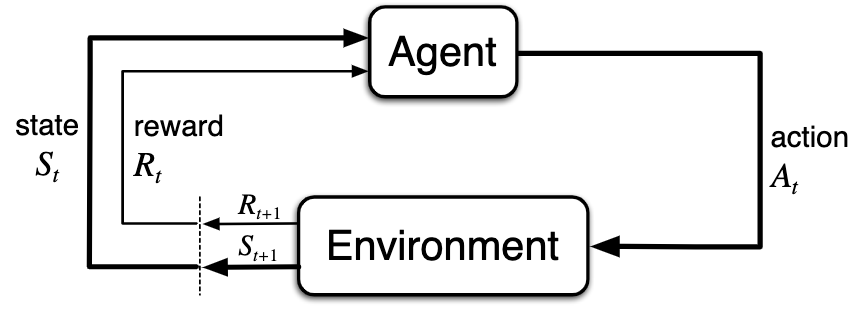
\includegraphics[width=0.8\linewidth]{figs/agent-env.png}
    \caption{Agent-Environment Interface}
    \label{fig:agent-env}
\end{figure}
resulting in a sequences of transitions
\begin{align}
    S_0, A_0, R_1, S_1, A_1, R_2, S_2, A_2, \cdots
\end{align}
Naturally, we can see that the interaction between an agent and the environment is time dependent. Note that a complete sequence of transitions is called an \texttt{episode}. That is, an episode records all transitions from the start state until the agent reaches the terminal state or the maximum number of timesteps. In addition, we define the reward to arrive one time step later than its corresponding action\footnote{Note that this is the conventional definition. It is also valid to define actions and rewards such that they occur in the same timestep.}.\\

Furthermore, we also see that the minimum necessary information for the agent to make a decision at each timestep $t$ is $S_t$. This indicates the agent-environment interaction follows the Markovian property
\begin{align}
    P(A_t|S_0, S_1, \cdots, S_t) &= P(A_t|S_t)
\end{align}
where the probability of selecting an action given current state is equivalent to the entire trajectory of states. That is, the action selection process is independent of the trajectory given the current state.

\subsection{Markov Decision Process (MDP)}

First, consider a Markov Reward Process (MRP), which is a formal way of describing an environment via a 4-tuple $(\mathcal{S},\mathcal{P},\mathcal{R},\gamma)$ where
\textbf{give ex of what S and A is}
\begin{itemize}
    \item $\mathcal{S}$ is a finite set of states
    \item $\mathcal{P}$ is the state transition probability matrix, and $P(S_{t+1}|S_t)$ is the probability of transition to the next state given the current state and action
    \item $\mathcal{R}$ is the reward function, and $\mathbb{E}[R_{t+1}|S_t]$ is the agent's expected reward given it is in some state
    \item $\gamma \in [0,1]$ is a discount factor applied on return $G_t$
\end{itemize}
and the dynamics of agent-environment satisfies Markov property. A discount factor $\gamma$ is introduced such that the return is modified from equation (\ref{eq:gamma1-return}) to
\begin{align}
    G_t &= R_{t+1} + \gamma R_{t+2} + \gamma^2 R_{t+3} + \cdots = \sum_{k=0}^\infty \gamma^k R_{t+k+1} \label{eq:discounted-return}
\end{align}
where the discount factor allows us to weight the importance of rewards proportionally according to how far in they are in the future. This is useful for several reasons. For example, the discount factor is mathematically convenient and avoids infinite sums in scenario where there isn't a terminal state. In addition, we may be motivated to weight future rewards less in situations where we favor immediate rewards.\\

The setup of MRP leads allows for a formal description to evaluate the quality of states. Specifically, the state-value function $V(s)$ is a function that evaluates the value of a state in the long run. That is, $V(s)$ is the expected value of the return given the agent starts at state $s$
\begin{align}
    V(s) = \mathbb{E}[G_t|S_t = s] \label{eq:v-func-org}
\end{align}
where the return can be expanded to derive a recursive relationship between pairs of consecutive states
\begin{align}
    V(s) &= \mathbb{E}[G_t|S_t = s] \nonumber\\
    &= \mathbb{E}[R_{t+1} + \gamma R_{t+2} + \gamma^2 R_{t+3} + \cdots | S_t = s] \nonumber\\
    &= \mathbb{E}[R_{t+1} + \gamma \left(R_{t+2} + \gamma R_{t+3} + \gamma^2 R_{t+4} + \cdots \right) | S_t = s] \nonumber\\
    &= \mathbb{E}[R_{t+1}+\gamma G_{t+1} | S_t = s] \nonumber\\
    &= \mathbb{E}[R_{t+1}+\gamma V(S_{t+1}) | S_t = s] \nonumber\\
    &= R_{t+1} + \gamma \sum_{s^\prime \in \mathcal{S}} P(S_{t+1}=s^\prime|S_t) V(s^\prime) \nonumber
\end{align}
as demonstrated in the second last expression. Also, note that last line of expression for $V(s)$ shows that the expectation is taken over transition probabilities from one state to the next. This implies a Markov Reward Process does not involve any decision making. That is, the agent does not have autonomy in the decision making process, and is merely transitioning between states as dictated by the environment's dynamics.\\

To complete the picture, we need to allow the agent to make its own decisions and quantify how the agent behaves when selecting an action. This leads to the policy of an agent $\pi(a|s)$, which is a distribution over all possible actions when in some state $s$
\begin{align}
    \pi(a|s) &= P(A_t=a|S_t=s)
\end{align}
Now, we can add the policy $\pi$ and some finite action space $\mathcal{A}$ to the original Markov \textit{Reward} Process to obtain a Markov \textit{Decision} Process (MDP). This results in a MDP 5-tuple $(\mathcal{S},\mathcal{A},\mathcal{P}_\pi,\mathcal{R}_\pi,\gamma)$ and a policy $\pi$, where the transition probability of a pair of states is
\begin{align}
    P_\pi(S_{t+1}|S_t,A_t) = \mathbb{E}_\pi [S_{t+1}|S_t,A_t] = \sum_a \pi(a|s) P(S_{t+1}|S_t=s,A_t=a) \nonumber
\end{align}
and expected reward given a state-action pair is
\begin{align}
    R_\pi(S_t,A_t) = \mathbb{E}_\pi [R_{t+1}|S_t,A_t] = \sum_a \pi(a|s) P(R_{t+1}|S_t=s,A_t=a) \nonumber
\end{align}
In addition, we define a action value function $Q_\pi(s,a)$, which evaluates the value of the state-action pair in the long run. That is, $Q(s,a)$ is the expected value of the return given the agent starts at state $s$ and takes action $a$, and follows policy $\pi$ from there onward
\begin{align}
    Q_\pi(s,a) &= \mathbb{E}_\pi[G_t|S_t=s,A_t=a] \nonumber\\
    &=\mathbb{E}_\pi[R_t+\gamma Q_\pi(S_{t+1},A_{t+1})|S_t=s,A_t=a] \nonumber
\end{align}
which also decomposes into a recursive relationship as demonstrated. Furthermore, we can redefine the value function $V_\pi(s)$ as the value estimate of a state under policy $\pi$. This allows us to relate state value function and action value function in the following sense
\begin{align}
    V_\pi(s) &= \mathbb{E}_\pi\left[R_t + \gamma V_\pi(S_{t+1}) | S_t = s\right]\\
    &= \sum_{a\in \mathcal{A}} \pi(a|s) Q_\pi(s,a) \nonumber \\
    Q_\pi(s,a) &= R_t + \gamma \sum_{s^\prime \in \mathcal{S}} P(S_{t+1}=s^\prime|S_t=s,A_t=a) V_\pi(s^\prime)
\end{align}
Notice that unlike the value function $V(s)$, probability transitions $\mathcal{P}$ and reward function $\mathcal{R}$ defined for a Markov \textit{Reward} Process, the corresponding functions for a Markov \textit{Decision} Process are taking expectations over $\pi$.

\subsection{A Note on Model-Based vs Model-Free RL}
Before discussing any RL algorithms in detail, we must first make a distinction between model-based and model-free reinforcement learning. These two implementations are fundamentally different in that a model-based RL agent explicitly models the environment it is interacting with. An example would be Dina-Q, an algorithm that models the environment and samples transitions from that model in order to ``plan" its moves in the real environment.\\

An example model-free RL agent would be the classical Q-learning agent, in which the agent has no knowledge regarding to the environment beyond the action value estimate which approximates the value of a certain state-action pair $Q_\pi(s,a)$.\\

In this report, we will focus on model-free RL agents, because the main school of thoughts regarding to multitask reinforcement learning deems explicit estimation for each task's environment too expensive and thus not scalable \cite{sharma2017online}.

\subsection{Policy Iteration} \label{sec:policy-iter}

\textbf{start with a clearer definition of policy iteration}
Policy iteration is one of the core ideas that guarantees the success of reinforcement learning agents. Policy iteration consists of two mechanisms, policy improvement and policy evaluation.\\

These two mechanisms are represented by four Bellman Equations \cite{sutton2018reinforcement} \cite{sutton1999between}
\begin{align}
    V_\pi(s)&=\mathbb{E}[R_{t+1}+\gamma V_\pi(S_{t+1})|S_t=s, A_t\sim \pi(S_t)] \label{eq:bellman1}\\
    Q_\pi(s,a)&=\mathbb{E}[R_{t+1}+\gamma Q_\pi(S_{t+1},A_{t+1})|S_t=s, A_t=a]\label{eq:bellman2}\\
    V_*(s)&=\argmax_a \mathbb{E}[R_{t+1}+\gamma V_*(S_{t+1})|S_t=s, A_t=a]\label{eq:bellman3}\\
    Q_*(s,a)&=\mathbb{E}[R_{t+1}+\gamma \max_{a^\prime} Q_*(S_{t+1},a^\prime)|S_t=s, A_t=a]\label{eq:bellman4}
\end{align}
, where $V_*$ and $Q_*$ represent the true values of states and state-action pairs. That is, they are the maximum state and action value functions over all policies
\begin{align}
    V_*(s) = \max_\pi V_\pi(s)\\
    Q_*(s,a) = \max_\pi Q_\pi(s,a)
\end{align}
Equations (\ref{eq:bellman1}) and (\ref{eq:bellman2}) are referred as predictions as they evaluate the value of a state or a state-action pair. For example, states closer to the goal state will have higher values than otherwise. Equations (\ref{eq:bellman3}) and (\ref{eq:bellman4}) are classically referred to as control or optimal policies. This is because given the true values $V_*$ and $Q_*$, the maximization over actions must yield the most amount of rewards.\\

% \subsection{Iterative Policy Evaluation}

Consider the goal to estimate the state-value function $V_\pi$ for an arbitrary policy $\pi$. We can start with an approximate value function $V_0$ and iteratively improve our estimation of $V_\pi$ via the following update rule
\begin{align}
    V_{k+1}(s) &= \mathbb{E}[R_{t+1}+\gamma V_k(S_{t+1})|S_t=s]\\
    &= \sum_a \pi(a|s)\sum_{s^\prime,r}P(s^\prime, r|s,a)[r+\gamma V_k(s^\prime)]
\end{align}
and arrive at the following algorithm \cite{sutton2018reinforcement} for estimating $V_\pi$
\begin{figure}[H]
    \center
    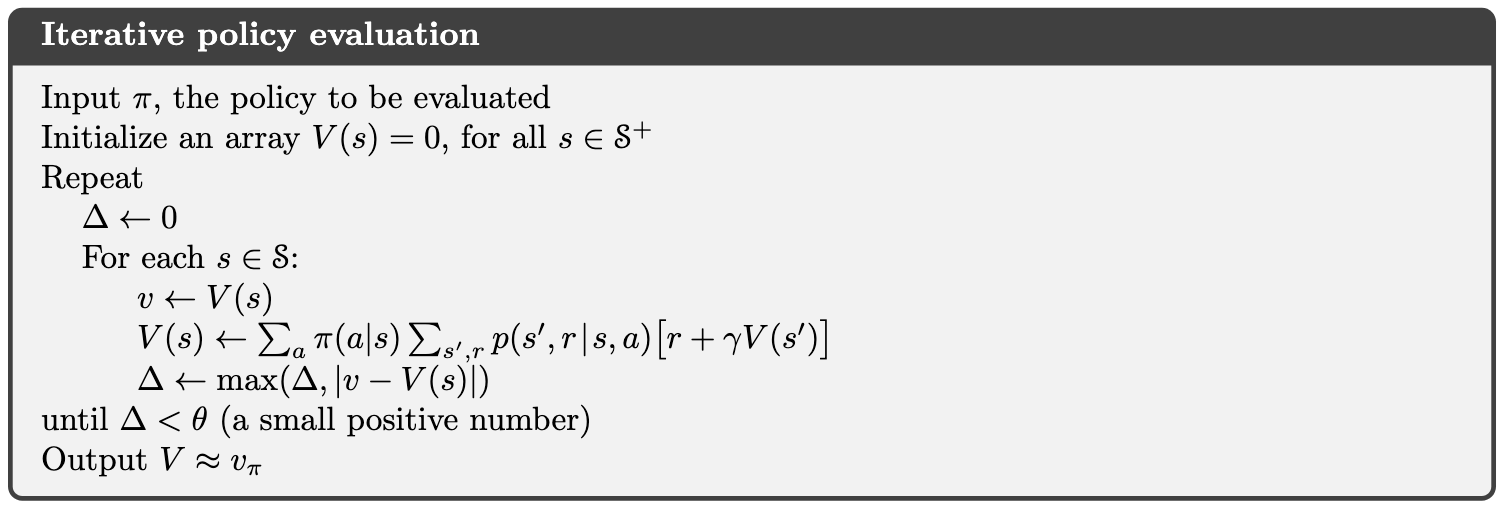
\includegraphics[width=0.8\linewidth]{figs/policy-eval.png}
    \label{fig:policy-eval}
\end{figure}
Now, if we consider the control equation (\ref{eq:bellman3}) maximizing over iterative states value estimates $V_{k+1}$ instead of the true values $V_*$, then the control equation becomes policy improvement. Let $V_{k+1}^\prime$ be the new policy derived from maximizing $V_{k+1}$. Then we are guaranteed to have $V_{k+1}^\prime \ge V_{k+1}$ according to the Policy Improvement Theorem \cite{sutton2018reinforcement}.\\

We can then estimate $V_{k+2}$ based on $V_{k+1}^\prime$ instead of $V_{k+1}$ to obtain the full cycle of policy iteration, as illustrated in the following diagram from David Silver's lecture notes \cite{silver2015}
\begin{figure}[H]
    \center
    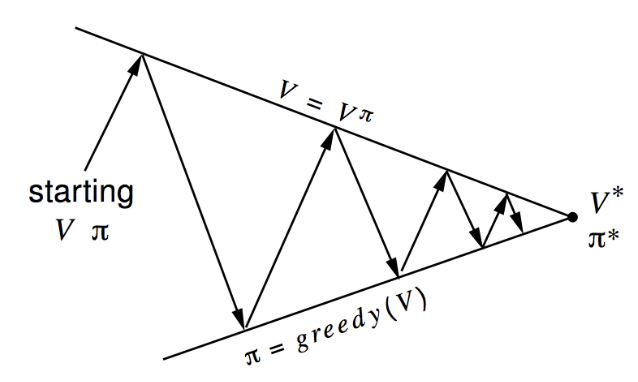
\includegraphics[width=0.45\linewidth]{figs/policy-iter.png}
    \caption{Visualization of Policy Iteration}
    \label{fig:policy-iter}
\end{figure}
As shown above, the iterative policy evaluation and improvement eventually converges to the optimal policy and state value function, where each iteration is a strict improvement over the last until convergence. A demonstration \cite{sutton2018reinforcement} of the policy iteration algorithm is shown in detail below
\begin{figure}[H]
    \center
    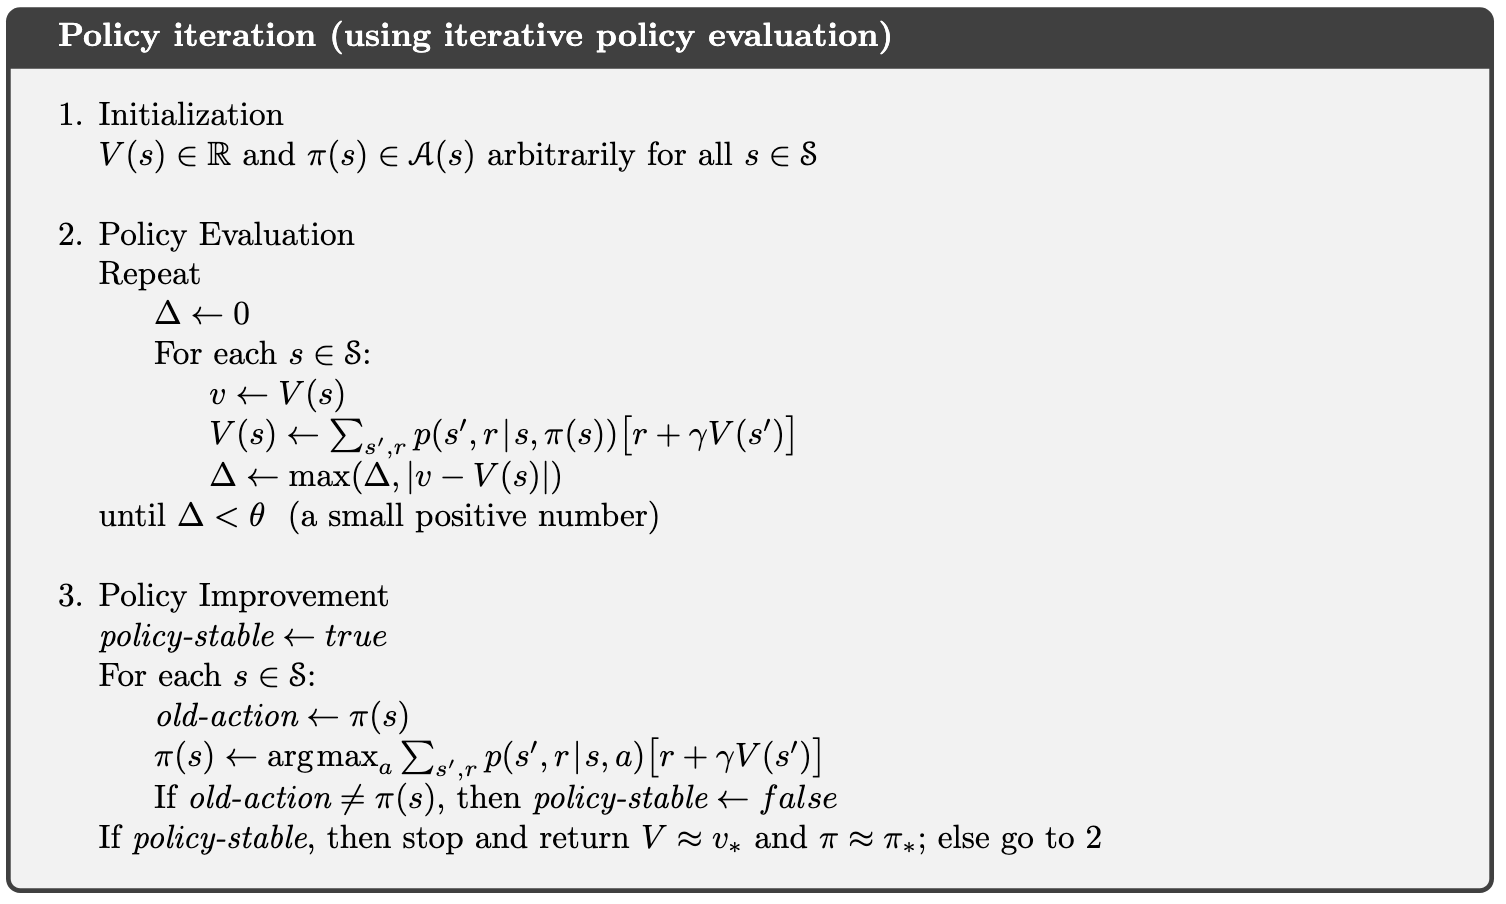
\includegraphics[width=0.8\linewidth]{figs/policy-iter-code.png}
    \label{fig:policy-iter-code}
\end{figure}
It should also be noted that all algorithms discussed in the following sections will be operating under the policy iteration framework.

\subsection{Table of definitions}
Here is a list of definitions and terminologies first introduced in the previous sections, and reiterated in a list for clarity. Note that we are following conventional statistical notations, in that all capital notations are \textbf{random variables} and all small letter notations are \textbf{constants}. 
\textbf{change the phrasing of arbitrary timestep of at time t}
\begin{center}
    \begin{tabular}{ l | p{10cm} }
    \small
    Terminology & Definition \\ \hline
    $t$ & Timestep of an episode \\
    $T$ & Number of timesteps reached until episode terminates \\
    $a$ / $A_t$ & An agent's action at an arbitrary timestep or at time $t$\\ 
    $R(s,a)$ / $R_t$ & Reward obtained during or after taking one step in the Markov Decision Process\\ 
    $s$ / $S_t$ & State of the agent at an arbitrary timestep or at time $t$ \\
    $\gamma$ & Discount value \\ 
    $\pi(a|s)$ & Policy of an agent \\ 
    $G_t$ & Cumulative rewards obtained from timestep $t$ until episode terminates \\ 
    $Q_\pi(s,a)$ & Value of a state-action pair under policy $\pi$ \\ 
    $V_\pi(s)$ & Value of a state under policy $\pi$ \\ 
    $Q_*$ & True/optimal action value function\\
    $V_*$ & True/optimal state value function
    \end{tabular}
\end{center}

\section{Q-learning}
First introduced by Watkins et al. \cite{watkins1992q}, Q-Learning is an off-policy model-free algorithm. Under the policy iteration framework, the representation of action values are updated according to the following equation:
\begin{align}
    Q(S_t,A_t) \leftarrow Q(S_t,A_t) + \alpha\left[R_{t+1}+\gamma \max_a Q(S_{t+1},a) - Q(S_t,A_t)\right] \label{eq:bellman-q-learning}
\end{align}
This is an off-policy algorithm because of the maximization of Q values over actions as supposed to using the agent's behaviour policy\footnote{Behaviour policy means the policy used by the agent to obtain a transition with the environment. In the case of the pseudocode above, it is the first line in the loop for each step of an episode.}. Below is Q-learning's pseudo-code extracted from Sutton and Barto \cite{sutton2018reinforcement}
\begin{figure}[H]
    \center
    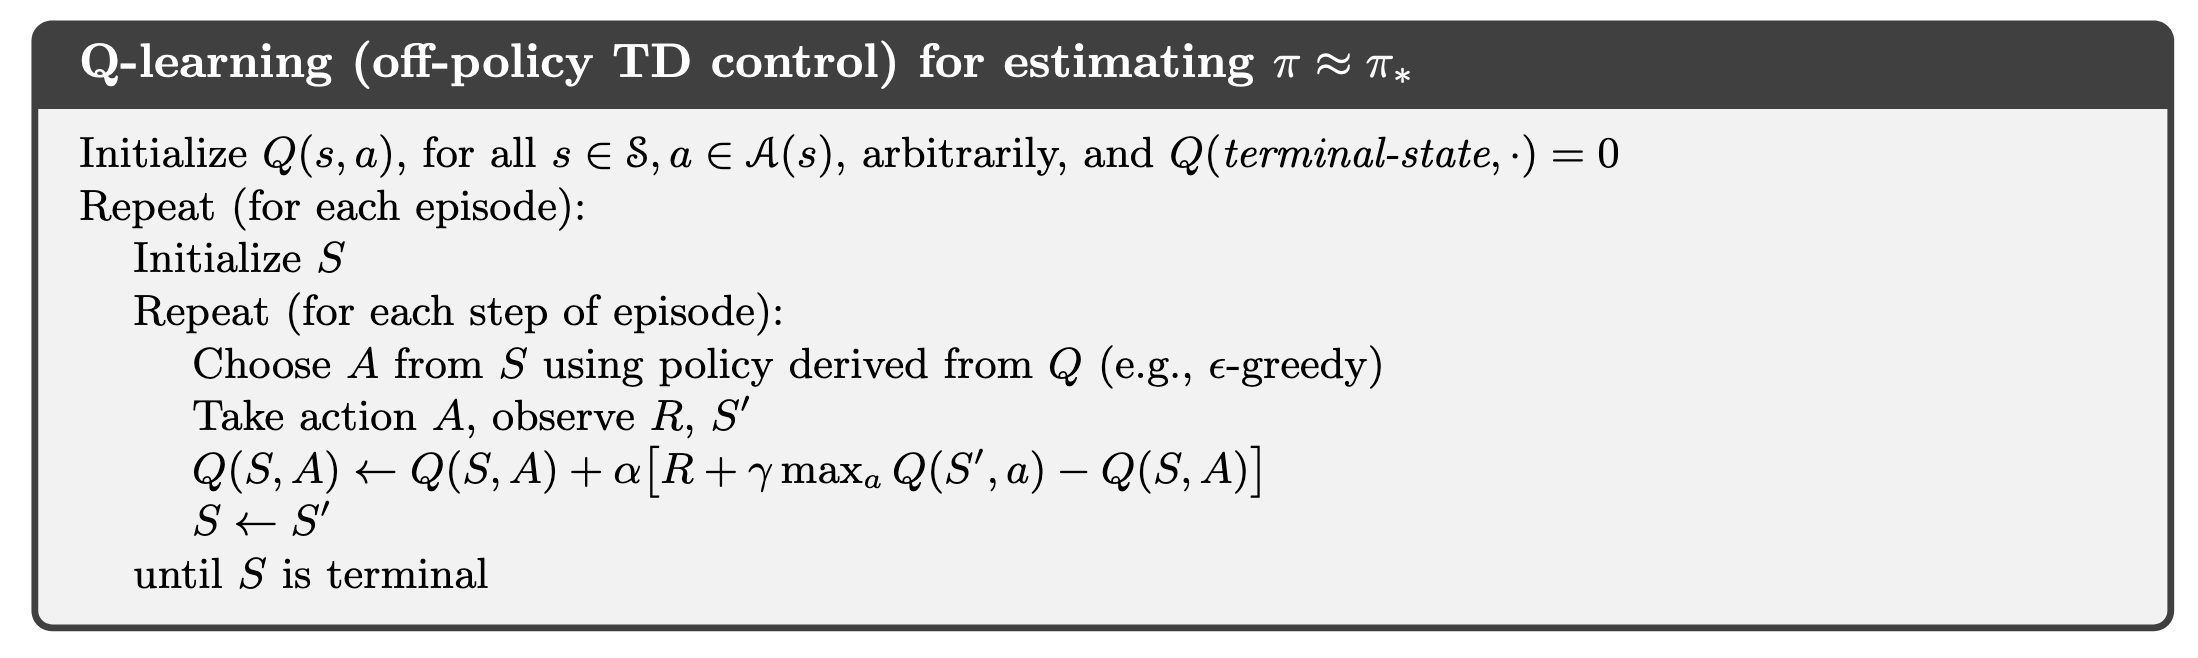
\includegraphics[width=0.9\linewidth]{figs/q_learning.png}
    \label{fig:qlearning}
\end{figure}
It is also known that this algorithm performs worse during training but does better than its counterparts in the testing phase.

\subsection{Deep Q-Learning (DQN)}\label{sec:DQN}

The concept of Q-learning is further developed into an architecture called Deep Q-learning (DQN) \cite{mnih2013playing}, which have demonstrated several advantages in replacing consecutive transitions with experience replay in the training process.\\

The idea of experience replay is to store the agent's interaction with the environment in a replay buffer and update state-action estimates by sampling from it. Mnih et al. \cite{mnih2013playing} suggests that using a replay memory improves data efficiency as each transition can be sampled multiple times. Furthermore, they argue that sampling decoupled transitions instead of learning from consecutive ones lowers the variance of action value estimates, and thus making the agent more robust to oscillating behaviour in performance. Below is the detailed psuedocode for DQN from Mnih et al. \cite{mnih2013playing}
\begin{figure}[H]
    \center
    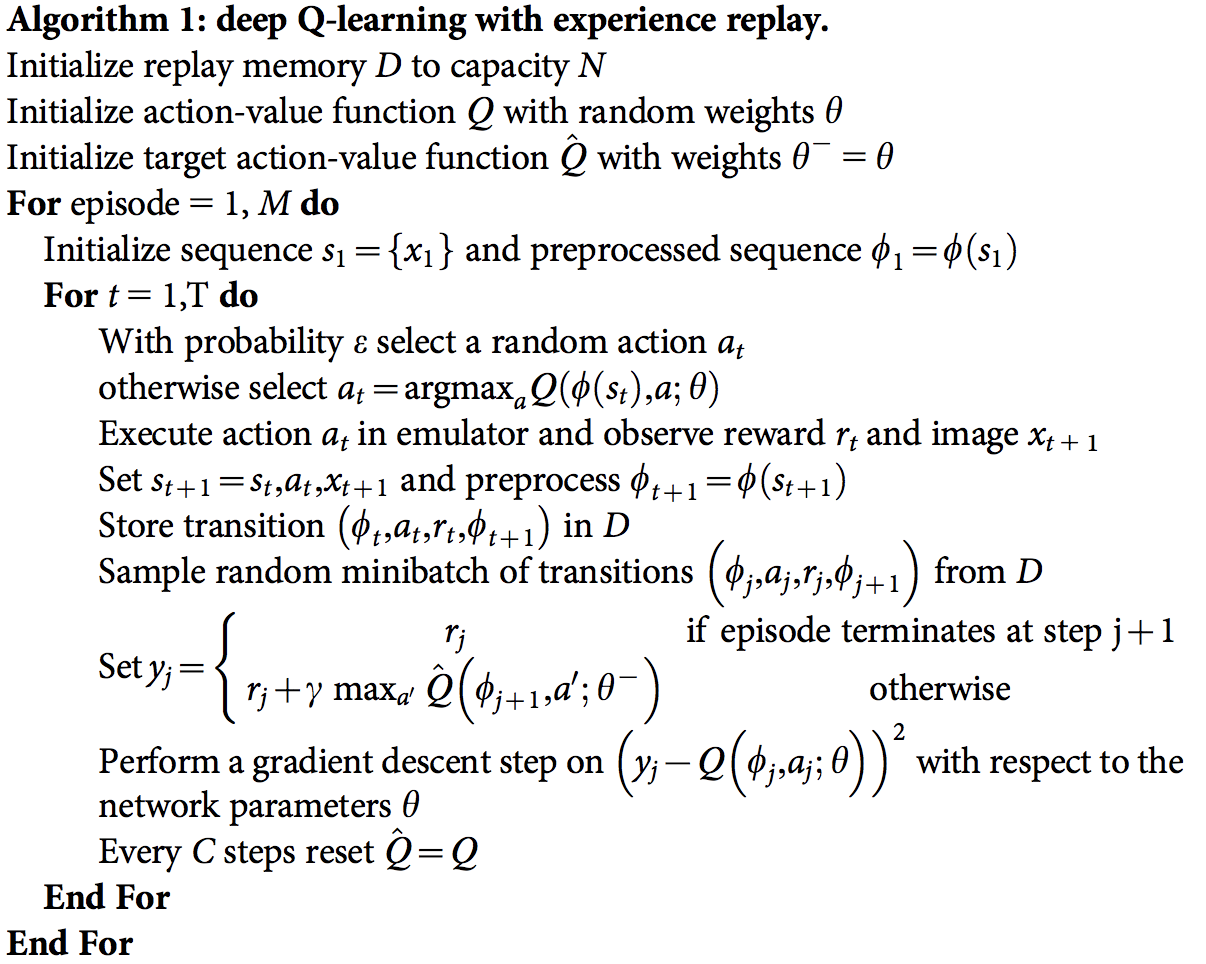
\includegraphics[width=0.7\linewidth]{figs/DQN_pseudocode.png}
    \label{fig:dqn}
\end{figure}

\section{Policy Gradient} \label{sec:policy-grad}

An alternative to value-based methods is policy-based methods, that is to directly optimize an agent's policy $\pi(a_t|s_t)$ directly rather than indirectly through, say $\epsilon$-greedy of action value estimates $Q(s_t,a_t)$.\\

One of the most compelling motivation for us to optimize against $\pi$ instead of $Q$ or $V$ is that in some circumstances, it is much easier for the agent to learn an optimal policy $\pi_*$ compared to learning an optimal value function $Q_*$ or $V_*$. For example, an agent may learn that the optimal policy is to always move right in a 2D platformer such as Sonic Mania (\ref{fig:sonic}), because the end of each level/stage is always to the right of its current position. Whereas, the accurate action values of each frame may be very difficult to learn due to the complex nature of the environment.
\begin{figure}[H]
    \center
    
\includegraphics[width=0.3\linewidth]{figs/sonic_mania.jpg}
    \caption{Sonic Mania, a 2D platformer}
    \label{fig:sonic}
\end{figure}
In addition, policy-based methods also has some advantages over value-based methods. Specifically, policy-based methods have better convergence properties, are effective in high dimensional or continuous spaces, and can learn stochastic policies. \textbf{ADD MORE CONTENT ELABORATING ADVANTAGES AND ALSO TALK ABOUT DISADVANTAGES}\\

Policy-based methods are better than the conventional $\epsilon$-greedy action selection simply because parameterization of action selection probabilities change smoothly with respect to its learned parameters \cite{sutton2018reinforcement}. In contrast, $\epsilon$-greedy policy can change drastically due to a small perturbation because of the \texttt{argmax} mechanism over action value estimates.\\

Moreover, policy-based methods are also convenient for learning the action selection probabilities in a very large or continuous action space. For example, a continuous action space can be parameterized as a Gaussian policy such that
\begin{align}
    \pi(a|s,\theta) &= \frac{1}{\sigma(s,\theta)\sqrt{2\pi}}\exp \left(-\frac{(a-\mu(s,\theta))^2}{2\sigma(s,\theta)^2}\right)
\end{align}
, where the $\pi$ in the denominator is the irrational number $3.14159\cdots$ and the mean $\mu$ and standard deviation $\sigma$ are parameterized by $\theta$.\\

Furthermore, an example where stochastic policies are required to solve a problem can be demonstrated in a simple maze (figure \ref{fig:alias}) from \cite{shani2005resolving}
\begin{figure}[H]
    \center
    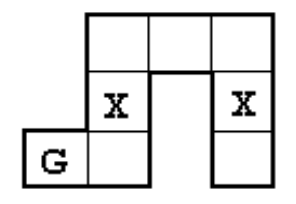
\includegraphics[width=0.3\linewidth]{figs/alias_world.png}
    \caption{Simple maze with alias states}
    \label{fig:alias}
\end{figure}
As seen above, the states with "x" are identical to an agent as both states represent a corridor where the agent can only move up or down. However, the agent has to move up in the right alias state and down in the left alias state in order to reach the goal state. A value-based method would have difficulty evaluating the state-action estimates of those states as they are aliases of each other. Whereas, a policy-based method may learn that the optimal policy is to remain stochastic at the alias states to guarantee convergence to the goal state.

\subsection{Problem setting} \label{sec:policy-grad-bandit}

Under the standard MDP framework, consider the goal to find the best $\theta$ given some policy $\pi_\theta(a_t|s_t)$. There are several common approaches to evaluate the quality of $\pi_\theta$ \cite{sutton2018reinforcement}, \cite{sutton2000policy}:
\begin{itemize}
    \item In an episodic environment, we can define performance as $J(\theta)=V_{\pi_\theta}(S_0)$
    \item For continuous problems without a terminal state, we can define performance as the average rate of reward per timestep $J(\theta)=\sum_s\mu(s)\sum_a\pi(a|s)\sum_{s^\prime,r}p(s^\prime,r|s,a)r$, where $\mu(s)$ is the stationary distribution\footnote{A stationary distribution of a MDP is defined as the expected number of visits for each state as the number of transitions approaches infinity.} of the MDP
\end{itemize}
Consider an episodic environment, then we can compute the gradient of $J(\theta)$ analytically, assuming $\pi_\theta$ is differentiable everywhere when $\pi_\theta \neq 0$. Furthermore, assume that we are dealing with a one-step episodic bandit scenario such that
\begin{align}
    J(\theta)=\mathbb{E}_{\mu, \pi}[R(S,A)]
\end{align}
, where the expectation is taken of $\mu$ and $\pi$, and $\mu$ is the stationary distribution of states and $\pi$ is the policy over actions.\\

Let $\pi_\theta = \pi$ to simplify notations, then the gradient w.r.t. the objective is
\begin{align}
\nabla_\theta \mathbb{E}[R(S,A)] &= \nabla_\theta \sum_s \mu(s) \sum_a \pi(a|s) R(s,a) \nonumber\\
&= \sum_s \mu(s) \sum_a \nabla_\theta \pi(a|s) R(s,a) \nonumber\\
&= \sum_s \mu(s) \sum_a \pi(a|s) \frac{\nabla_\theta \pi(a|s)}{\pi(a|s)} R(s,a) \label{eq:log-trick}\\
&= \mathbb{E}[\nabla_\theta \log \pi(a|s) R(s,a)] \nonumber
\end{align}
, where the transition from the second last (\ref{eq:log-trick}) to the last line is commonly referred to as the score-function trick or log likelihood ratio identity. This expression can the be sampled and updated incrementally via stochastic gradient descent.

\subsection{Policy Gradient on Trajectories}

Now consider instead of a one-step bandit scenario, we have an episodic environment that lasts over multiple steps. That is, each episode consists of a trajectory $\zeta = S_0, A_0, R_1, S_1, A_1, R_2, S_2 \cdots$ with return as $G(\zeta)$. Assume the discount factor $\gamma = 1$ for simplicity, then the policy gradient becomes
\begin{align}
\nabla_\theta J_\theta (\pi) &= \nabla_\theta \mathbb{E}[G(\zeta)]\nonumber\\
&= \mathbb{E}[G(\zeta)\nabla_\theta \log P(\zeta)] \label{eq:policy-grad-traj}
\end{align}
via the score function trick as mentioned in (\ref{eq:log-trick}). Expanding the derivative w.r.t. to $\log P(\zeta)$ gives
\begin{align}
    \nabla_\theta \log P(\zeta) &= \nabla_\theta \log \left[P(S_0)\pi(A_0|S_0) \prod_{t\ge1} P(S_t|S_{t-1},A_{t-1})\pi(A_t|S_t) \right]\nonumber\\
    &=\nabla_\theta \left[\log P(S_0) + \log \pi(A_0|S_0) + \sum_{t\ge 1}\log P(S_t|S_{t-1},A_{t-1}) + \sum_{t\ge 1}\log \pi(A_t|S_t)\right]\nonumber\\
    &= \nabla_\theta \left[\sum_{t\ge0} \log \pi (A_t|S_t)\right]\nonumber
\end{align}
Substituting the expression above back into the partial derivative w.r.t. the performance of the policy
\begin{align}
    \nabla_\theta J_\theta(\pi) &= \mathbb{E}\left[G(\zeta) \nabla_\theta \sum_{t\ge0} \log \pi(A_t|S_t)\right]\nonumber\\
    &=\mathbb{E}\left[\sum_{t\ge0}R_{t+1} \nabla_\theta \sum_{t\ge0} \log \pi(A_t|S_t)\right] \nonumber
\end{align}
Also, since $\sum_{t=0}^k R_{t+1}$ doesn't depend on actions $A_{k+1}, A_{k+2}, \cdots$, we can rewrite and simplify (\ref{eq:policy-grad-traj})
\begin{align}
\nabla_\theta J_\theta(\pi) &= \mathbb{E}\left[\sum_{t\ge0} R_{t+1} \nabla_\theta \sum_{t\ge0} \log \pi(A_t|S_t)\right] \nonumber\\
&= \mathbb{E}\left[\sum_{t\ge0} \nabla_\theta \log \pi(A_t|S_t) \left(\sum_{i=t} R_{i+1}\right)\right] \label{eq:REINFORCE}
\end{align}
Note that if $\gamma \neq 1$, then
\begin{align}
\nabla_\theta J_\theta(\pi) = \mathbb{E}\left[\sum_{t\ge0}\nabla_\theta  \log \pi(A_t|S_t) \left(\sum_{i=t} \gamma^{i-t} R_{i+1}\right) \right] \label{eq1}
\end{align}

\subsection{Policy Gradient Theorem}

The method of rewriting the expression of policy gradient stated in the context of a one-step and n-step bandit in the previous sections can be generalized into a theorem. Specifically, policy gradient theorem states that \cite{sutton2018reinforcement} given any differentiable policy $\pi(s|a)$ and any policy objective function $J(\theta)$ mentioned above, the policy gradient is
\begin{align}
    \nabla_\theta J(\theta) &= \nabla_\theta \sum_s \mu(s) \sum_a \pi(a|s) R(s,a) \nonumber\\
    &= \mathbb{E}_{\pi}[\nabla_\theta \log \pi(a|s) Q_{\pi}(s,a)] \label{eq:policy-grad}
\end{align}
Note that rewriting the gradient of the expected value into expected value of a gradient is important as the second expression circumvents the problem of depending on the action selection and the stationary distribution of states, which are both determined by the policy $\pi(a|s)$. 

\subsection{REINFORCE}

One of the earliest policy gradient algorithms is the REINFORCE algorithm \cite{williams1992simple}, as state in equation \ref{eq:REINFORCE} in the previous sections
\begin{align}
    \nabla_\theta J(\theta) &= \mathbb{E}_{\pi_\theta}[\nabla_\theta \log \pi_\theta(a|s) Q_{\pi_\theta}(s,a)] \nonumber\\
    &= \mathbb{E}_{\pi_\theta}[\nabla_\theta \log \pi_\theta(a|s) G_t]
\end{align}
, where $G_t = \sum_{t^\prime > t} R_{t^\prime}$ is the return or cumulative reward from time timestep $t$ onward. This is because $\mathbb{E_{\pi_\theta}}[G_t|S_t,A_t] = Q_{\pi_\theta}(S_t,A_t)$ by definition.\\

Note that REINFORCE is a Monte-Carlo algorithm, in that it uses the entire trajectory of returns up until the final transition of the episode. Here is the pseudocode from Sutton and Barto \cite{sutton2018reinforcement}
\begin{figure}[H]
    \center
    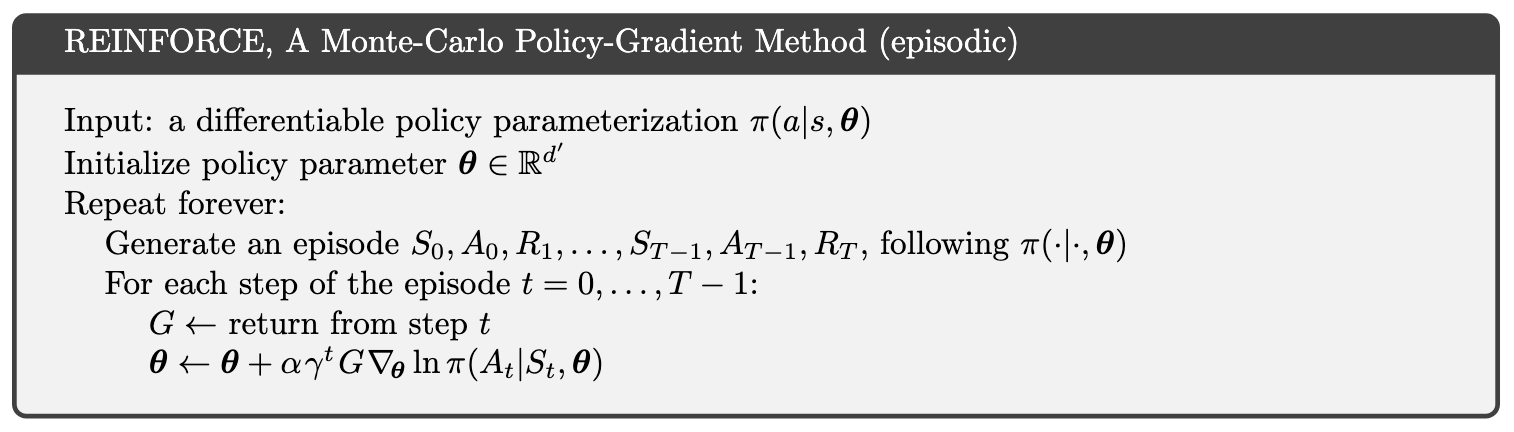
\includegraphics[width=0.9\linewidth]{figs/REINFORCE.png}
    \label{fig:REINFORCE}
\end{figure}
\section{Advantage Actor Critic Model (A2C)}

Another well known variant of policy gradient is the Advantage Actor-Critic (A2C) algorithm, which is a union between policy gradient and state value function estimate. That is, the policy gradient plays the role of an actor and the state value function estimate plays the role of the critic by evaluating the value of states.\\

Consider using the same policy gradient as REINFORCE, and then construct a critic which models $Q_\pi(s,a)$ explicitly with another function approximation, such as a neural network\footnote{Note that actor and critic networks can either be represented by the same or separate neural network \cite{haarnoja2018soft1}.} such that $Q_w(s,a) \approx Q_\pi(s,a)$ for some parameters $w$. Then
\begin{align}
    \nabla_\theta J(\theta) &= \mathbb{E}_{\pi_\theta}[\nabla_\theta \log \pi_\theta(a|s) Q_{\pi_\theta}(s,a)] \nonumber\\
    &= \mathbb{E}_{\pi_\theta}[\nabla_\theta \log \pi_\theta(a|s) Q_w(s,a)]
\end{align}
, where $Q_w(s,a)$ is analogous to policy evaluation as mentioned in section \ref{sec:policy-iter}. Note that the transition from the first to the second line is only equivalent when the state-value function satisfies the Compatible Function Approximation Theorem \cite{thomas2017policy} \cite{silver2015}. Specifically, the theorem is only satisfied if and only if the value function is compatible with the policy and the value function parameters $w$ minimizes a least squares loss function.\\

We can then update the parameters $w$ by performing 1-step TD-learning via least squares
\begin{align}
    L(Q_w)&=\frac{1}{2}\mathbb{E}\left[(\hat{Q}_w(S_t,a)-Q_w(S_t, a))^2\right]\nonumber\\
    \hat{Q}_w(S_t, a) &= R_{t+1} + \gamma Q_w(S_{t+1},A_{t+1}) \nonumber\\
    \text{where } A_{t+1} &\sim \pi \nonumber
\end{align}
Furthermore, subtracting $Q_w(s,a)$ by a baseline can reduce the variance of the policy gradient, which is allowed as the expectation of the gradient remains the same. For example, let $B(s)$ be the baseline we wish to subtract $Q_\pi(s,a)$ from, then
\begin{align}
    \mathbb{E}[\nabla_\theta \log \pi(a|s)B(s)] &= \sum_s \mu(s) \sum_a \nabla_\theta \pi(a|s)B(s) \nonumber\\
    &=\sum_s \mu(s) B(s) \nabla_\theta \sum_a \pi(a|s) \label{eq:policy-baseline}\\
    &= 0 \nonumber
\end{align}
, where the baseline is moved outside of the partial derivative because it is independent of $\theta$. A typical baseline to use is the state-value estimate $V_v(s)$, which can also be estimated using another explicit function approximation with parameters $v$. Rewriting the policy gradient obtains the following 
\begin{align}
    \nabla_\theta J_\theta(\pi) &= \mathbb{E}\left[\sum_{t\ge0} \nabla_\theta \log \pi(A_t|S_t) (Q_w(S_t, A_t) - V_v (S_t))\right] \label{eq:AC-Q-V-params}\\
    &= \mathbb{E}\left[\sum_{t\ge0} \nabla_\theta \log \pi(A_t|S_t) A(S_t, A_t)\right]
\end{align}
, where $A(S_t, A_t)$ is called the advantage function as it measures the difference between the value of a particular state-action pair versus state, which can be interpreted as the average value across all actions of the state. Again, both $Q_w$ and $V_v$ can be updated separately via 1-step or n-step TD learning.\\

However, there is an alternative way of estimating the advantage function which is more efficient. Specifically, we know that the TD error $\delta_{\pi_\theta}$ is an unbiased estimate \cite{silver2015} of the advantage function given the true value function $V_{\pi_\theta}(s)$
\begin{align}
    \mathbb{E}[\delta_{\pi_\theta}|s,a] &= \mathbb{E}[r + \gamma V_{\pi_\theta}(s^\prime) - V_{\pi_\theta}(s)|s,a] \nonumber\\
    &= \mathbb{E}[r + \gamma V_{\pi_\theta}(s^\prime)|s,a] - V_{\pi_\theta}(s) \nonumber\\
    &= Q_{\pi_\theta}(s,a) - V_{\pi_\theta}(s)\nonumber\\
    &= A_{\pi_\theta}(s,a) \nonumber
\end{align}
Thus the advantage function can be replaced by the TD error
\begin{align}
    \nabla_\theta J_\theta(\pi) &= \mathbb{E}\left[\sum_{t\ge0} \nabla_\theta \log \pi(A_t|S_t) \delta_v\right] \label{eq:A2C-policy-grad}
\end{align}
where $\delta_v = r + \gamma V_v(s^\prime) - V_v(s)$ is the estimate of $\delta_{\pi_\theta}$. Note that this is more efficient as only one set of parameters $v$ need to be maintained instead of two. Similarly, an n-step TD estimate can be used instead, defining the loss on $V_v$ as
\begin{align}
    L(V_v) &= \frac{1}{2}\mathbb{E}\left[\Big(\delta_{v,t+n}\Big)^2\right]\\
    &= \frac{1}{2}\mathbb{E}\left[\Big(R_{t+1}+ \gamma R_{t+2} + \cdots + \gamma^{n-1}V_v(S_{t+n})-V_v(s_t)\Big)^2\right]
\end{align}
with an identical policy gradient as mentioned above except replacing $\delta_v$ with $\delta_{v,t+n}$. Finally, here is the detail pseudocode for a one-step A2C obtained from Sutton and Barto \cite{sutton2018reinforcement}
\begin{figure}[H]
    \center
    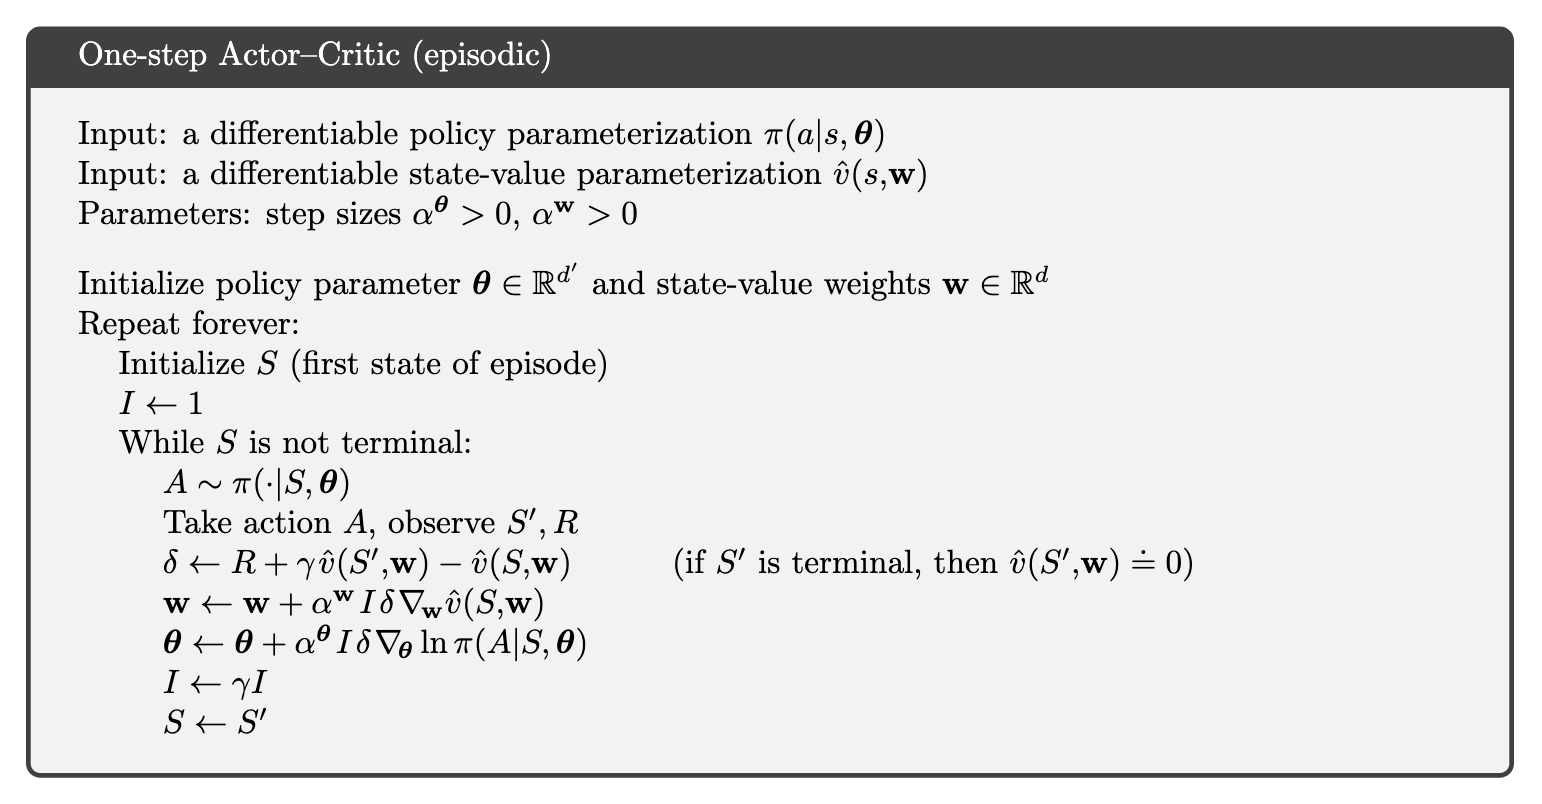
\includegraphics[width=1\linewidth]{figs/A2C.png}
    \label{fig:A2C}
\end{figure}

\subsection{Asynchronous Advantage Actor-Critic (A3C)}

Asynchronous Advantage Actor-Critic (A3C) is a variant of A2C in that there are multiple workers each learning on a different trajectory, and what is learned is shared to the master node. The policies of master and worker nodes are updated in an asynchronous manner, making the learning more stable. Mnih et al. \cite{mnih2016asynchronous} argues this variant of actor-critic learns faster than the conventional A2C framework at a lower computational cost. Below is a pseudocode for A3C from the original work \cite{mnih2016asynchronous}
\begin{figure}[H]
    \center
    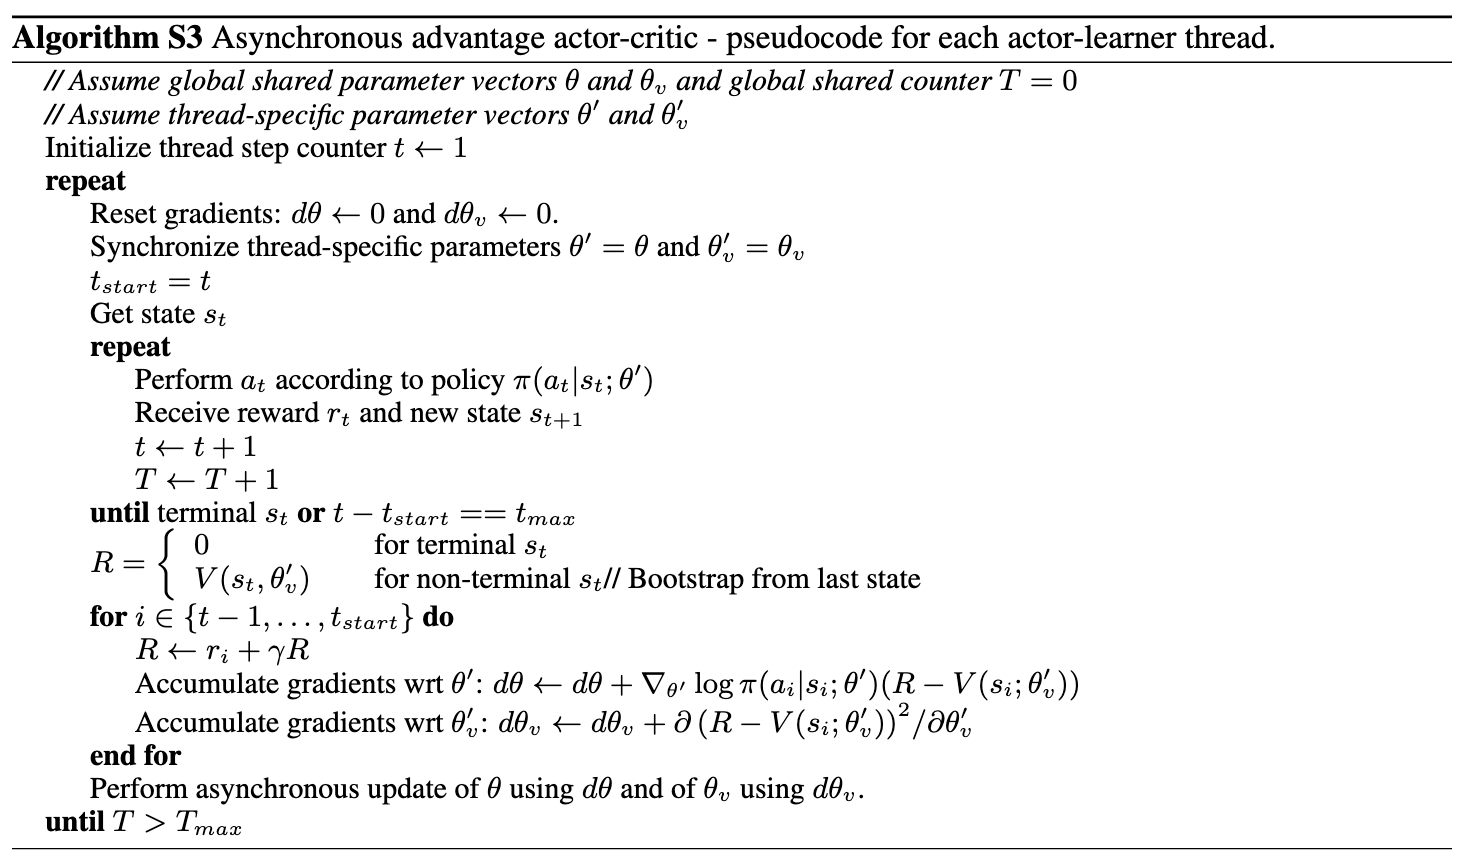
\includegraphics[width=.9\linewidth]{figs/A3C.png}
    \label{fig:A3C}
\end{figure}

\section{Maximum Entropy Reinforcement Learning}
\subsection{Bandit setting}
Consider the Bandit setting where each episode is 1 timestep, and at each time $t$, we choose an action $a$ and receive a reward $r$ sampled from $P(r|a)$ and rewards distribution is unknown.\\

Define $\Bar{r}(a)=\mathbb{E}(r|a)=\sum_r rP(r|a)$ and let $\pi$ be the policy representing probabilities over actions. Then the expected per-timestep reward of $\pi$ is
$$\mathbb{E}[r]=\sum_a \pi(a)\Bar{r}(a)$$
Conventionally, we would want to maximize the expected rewards as stated above. However, under entropy regularized setting, we want to maximize $\eta(\pi)$, and entropy version of the original objective instead:
\begin{align}
    \eta(\pi)&=\mathbb{E}_\pi[r]-\frac{1}{\beta}\text{KL}[\pi\|\pi_0]\\
    &= \mathbb{E}_\pi\left[\Bar{r}(a) - \frac{1}{\beta}\log \frac{\pi(a)}{\pi_0(a)}\right]\\ 
    \nonumber
\end{align}
, where $\pi_0$ \footnote{Note that the original work \cite{schulman2017equivalence} uses $\bar{\pi}$ as the reference policy. This is changed to keep notations consistent with the multitask algorithms.} is some reference policy, and $\frac{1}{\beta}$ is referred to as a temperature parameter\footnote{Note that the temperature coefficient is changed from $\tau$ to $\frac{1}{\beta}$ to keep notations consistent.}. From Schulman et al. \cite{schulman2017equivalence}, $\eta(\pi)$ is maximized by the following quantity
\begin{align}
    \pi_{\Bar{r}}^B = \frac{\pi_0(a)\exp (\beta \Bar{r}(a))}{\mathbb{E}_{\pi_0}[\exp (\beta \Bar{r}(a^\prime))]} \label{eq2.3}
\end{align}

% This can be shown by looking at the KL divergence between $\pi$ and $\pi_{\Bar{r}}^B(a)$

% \begin{align}
%     \text{KL}[\pi\|\pi_{\Bar{r}}^B]&=\mathbb{E}_\pi [\log \pi(a)-\log \pi_{\Bar{r}}^B(a)]\\
%     &=\mathbb{E}_\pi \Big[\log \pi(a)-\log \pi(a) - \Bar{r}(a)/C_\text{KL} + \log \mathbb{E}_{\pi_0}[\exp(\Bar{r}(a)/C_\text{KL}]\Big]\\
%     &=\text{KL}[\pi\|\pi_0] - \mathbb{E}_\pi [\Bar{r}(a)/C_\text{KL}] + \log \mathbb{E}_{\pi_0}[\exp (\Bar{r}(a)/C_\text{KL})]
% \end{align}

% Rearranging the terms gives

% \begin{align}
%     \mathbb{E}_\pi(\Bar{r}(a)) - C_\text{KL}\text{KL}[\pi\|\pi_0] &= C_\text{KL} \log \mathbb{E}_{\pi_0} [\exp (\Bar{r}(a)/ C_\text{KL})] - C_\text{KL}\text{KL}[\pi\|\pi_{\Bar{r}}^B]\label{eq2.7}\\ 
%     &=\eta(\pi) \nonumber
% \end{align}

% Hence the quantity on the R.H.S. of (\ref{eq2.7}) is maximized when $\pi=\pi_{\Bar{r}}^B$.\\

\subsection{Solving entropy-regularized bandit problem}

The derivation in the previous section assumes that the reward distribution is known s.t. $\Bar{r}$ is known. If it is not known initially, then we usually solve the entropy-regularized bandit problem either via policy-based or value-based methods.\\

For a policy-based approach, we can sample the policy gradient as mentioned previously in section \ref{sec:policy-grad}, as an unbiased estimate. Parameterizing $\pi$ with $\theta$ gives the following gradient as stated by Schulman et al. \cite{schulman2017equivalence}
\begin{align}
    \nabla_\theta \eta(\pi_\theta)&=\mathbb{E}\left[\nabla_\theta \log \pi_\theta(a)r-\frac{1}{\beta}\nabla_\theta\text{KL}[\pi_\theta\|\pi_0]\right]
\end{align}
where the derivation is analogous to the unregularized bandit problem as demonstrated in section \ref{sec:policy-grad-bandit}. For a value-based approach, we can parameterize the value function $Q(a)$ with $\theta$, and optimize the state-value estimates under the actor-critic framework via least squares loss
\begin{align}
    L(\pi_\theta)&=\frac{1}{2}\mathbb{E}\left[(Q_\theta(a)-r)^2\right]
\end{align}
where the gradient of the loss w.r.t $\theta$ is
\begin{align}
    \nabla L(\pi_\theta)&=\frac{1}{2}\mathbb{E}\left[\nabla_\theta Q_\theta(a)(Q_\theta(a)-r)\right]
\end{align}

\textbf{FOR VALUE BASED METHODS...}

\subsection{Setup for entropy-regularized MDPs} \label{sec:entropy-mdp}

Consider the entropy-regularized version of MDP\footnote{Note that this section assumes at $t=0$ there in an action $a_0$ and reward $r_0$, and that rewards are obtained on the same time step as the action.} such that the conventional discounted return is modified into
\begin{align}
    G_t &= \sum_{t=0}^\infty \gamma^t\left(R_t-\frac{1}{\beta}\text{KL}[\pi_\theta(\cdot |S_t)\|\pi_0(\cdot |S_t)]\right)\nonumber\\
    &= \sum_{t=0}^\infty \gamma^t\left(R_t-\frac{1}{\beta}\text{KL}_t\right)\label{eq:reg_rwd}
\end{align}
, where $\text{KL}[\pi_\theta(\cdot |S_t)\|\pi_0(\cdot |S_t)] = \text{KL}_t$. Based on this modified return, the new entropy state-value function and entropy state action-value function are
\begin{align}
    V_{\pi_\theta}(s)&=\mathbb{E}[G_t|S_t=s] \nonumber\\
    &=\mathbb{E}\left[\sum_{t=0}^\infty\gamma^t\left(R_t-\frac{1}{\beta}\text{KL}_t\right)\Big|S_t=s\right]\label{eq2.11}\\
    Q_{\pi_\theta}(s,a)&=\mathbb{E}[G_t|S_t=s,A_t=a] \nonumber\\
    &=\mathbb{E}\left[R_0+\sum_{t=1}^\infty \gamma^t\left(R_t - \frac{1}{\beta}\text{KL}_t\right)\Big|S_t=s,A_t=a\right]\label{eq2.12}
\end{align}

Note that the Q-function does not include the KL penalty for the first reward term, because it is defined to be independent of the action $A_0$ \cite{schulman2017equivalence}. This makes some expressions later simpler, and leads to the following between $Q_{\pi_\theta}$ and $V_{\pi_\theta}$
\begin{align}
    V_{\pi_\theta}(s) = \mathbb{E}[Q_{\pi_\theta}(s,a)]-\frac{1}{\beta}\text{KL}[\pi_\theta(\cdot|s)\|\pi_0(\cdot|s)]
\end{align}

\subsection{Soft Q-learning (SQL)} \label{sec:SQL}

% SQL was talked about in details from this paper \cite{zhang2019pretrain} and \cite{haarnoja2018soft} and...

Under the framework of entropy regularized rewards as stated in (\ref{eq:reg_rwd}), SQL minimizes the following loss function \cite{schulman2017equivalence}
% \begin{align} \label{SQL-eqs}
%     L(Q) &= \mathbb{E}\left[\frac{1}{2}\left(Q(s_t,a_t)-y_t\right)^2\right]\\
%     y_t &= \begin{cases} r_t + \gamma V(s_{t+1})&\mbox{1-step TD-learning} \\
%     \frac{1}{\beta}\text{KL}_t + V(s_t) + \sum_{d=0}^{n-1}\gamma^d \delta_{t+d}& \mbox{n-step TD-learning} \end{cases}\\
%     \text{where } V(s_{t+1}) &= 1/\beta \log \sum_{a^\prime} \pi_0(a^\prime|s_t) \exp{(\beta Q(s,a^\prime))} \label{eq:SQL-v-est}\\
%     \text{KL}_t &= \text{KL}[\pi_\theta(a_t | s_t)\|\pi_0(a_t | s_t)]\\
%     \delta_t &= (r_t - \frac{1}{\beta}\text{KL}_t) + \gamma V(s_{t+1}) - V(s_{t}) \label{eq:reg-td-error}
% \end{align}
\begin{align} \label{SQL-eqs}
    L(Q) &= \mathbb{E}\left[\frac{1}{2}\left(Q(s_t,a_t)-y_t\right)^2\right]\\
    y_t &= \begin{cases} r_t + \gamma V(s_{t+1})&\mbox{1-step TD-learning} \\
    \frac{1}{\beta}\text{KL}_t + \sum_{d=0}^{n-1}\gamma^d (r_{t+d}-\frac{1}{\beta}\text{KL}_{t+d}) + \gamma^n V(s_{t+n})& \mbox{n-step TD-learning} \end{cases}\\
    \text{where } V(s_{t+1}) &= 1/\beta \log \sum_{a^\prime} \pi_0(a^\prime|s_t) \exp{(\beta Q(s,a^\prime))} \label{eq:SQL-v-est}\\
    \text{KL}_t &= \text{KL}[\pi_\theta(a_t | s_t)\|\pi_0(a_t | s_t)]\nonumber
\end{align}
% \delta_t &= (r_t - \frac{1}{\beta}\text{KL}_t) + \gamma V(s_{t+1}) - V(s_{t}) \label{eq:reg-td-error}
Note the major difference between conventional DQN as mentioned in section \ref{sec:DQN} is in the definition of the Bellman equation. In the conventional DQN, the state-value estimate is maximizing over actions, as stated in equation (\ref{eq:bellman-q-learning})
\begin{align}
    V(s_t) = \max_{a_t}(Q(a_t,s_t)) \nonumber
\end{align}
whereas SQL's state-value estimate (\ref{eq:SQL-v-est}) is as defined above. 

\subsection{Actor-Critic with Regularized Rewards} \label{sec:ac_reg}

Actor-Critic under the context of a entropy regularized rewards often \cite{williams1992simple} have the following policy gradient estimate
\begin{align}
    \mathbb{E}\left[\nabla_\theta \log \pi_\theta(a_t|s_t)\sum_{t^\prime \ge t} R_{t^\prime} - \frac{1}{\beta}\nabla_\theta \text{KL}_t\right]
\end{align}
However, Schulman et al. \cite{schulman2017equivalence} states that the objective above is not accurate because the entropy regularization only applies to the current timestep, and that a proper entropy regularized policy gradient would include entropy regularization in the entire trajectory beginning from timestep $t$. Thus resulting in the following alternative
\begin{align}
    g_\gamma(\pi_\theta)&=\mathbb{E}\left[\sum_{t=0}^\infty\nabla_\theta \log \pi_\theta(a_t|s_t)\left(R_0 + \sum_{d=1}^\infty \gamma^d \left(R_{t+d}-\frac{1}{\beta}\text{KL}_{t+d}\right)-\frac{1}{\beta}\nabla_\theta \text{KL}_{t} \right)\right] \label{eq2.14temp}\\
    &=\mathbb{E}\left[\sum_{t=0}^\infty\nabla_\theta \log \pi_\theta(a_t|s_t)(Q_{\pi_\theta}(S_t,A_t)-V_{\pi_\theta}(S_t))-\frac{1}{\beta}\nabla_\theta \text{KL}_t\right] \label{eq2.15temp}
\end{align}
, where (\ref{eq2.14temp}) and (\ref{eq2.15temp}) are expressed in terms of empirical returns and values functions (\ref{eq2.11}) and (\ref{eq2.12}). We can then approximate $g_\gamma$ via n-step methods \cite{mnih2016asynchronous} or TD-$\lambda$ methods \cite{schulman2015high} to truncate the return and lower the variance. Schulman et al. \cite{schulman2017equivalence} chose to focus on the n-step methods and arrived at the following estimation of regularized policy gradient
\begin{align}
    \mathbb{E}\left[\nabla_\theta \log \pi_\theta(A_t|S_t)\delta_{t+n}\right]
\end{align}
% \sum_{d=0}^{n-1}\gamma^d\delta_{t+d}
, where $\delta_{t+n}$ is the n-step temporal difference as stated in equation (\ref{eq:A2C-policy-grad}). Then the corresponding optimization for the critic or the value function estimate is
\begin{align}
    L(V) &= \mathbb{E}\left[\frac{1}{2}(V(S_t)-y_t)^2\right]\\
    \text{where } y_t &=\frac{1}{\beta}\text{KL}_t + \sum_{d=0}^{n-1} \gamma^d\left(R_{t+d}-\frac{1}{\beta}\text{KL}_{t+d}\right) + \gamma^n V(S_{t+n})
\end{align}
% = V(S_t) + \sum_{d=0}^{n-1}\gamma^d \delta_{t+d}
and $V(s)$ is as stated previously in equation (\ref{eq:SQL-v-est}).

\subsection{Equivalence Between SQL and AC With Regularized Rewards}

It is important to note that the SQL framework and AC with regularized rewards are equivalent under the objective functions stated in sections \ref{sec:SQL} and \ref{sec:ac_reg}. Specifically, Schulman et al. \cite{schulman2017equivalence} states that defining $V_\theta$ and $\pi_\theta$ as the following of any parameterized $Q$-function $Q_\theta$
\begin{align}
    V_\theta(s)&=\frac{1}{\beta}\log \mathbb{E}[\exp(\beta Q_\theta(s,a))]\\
    \pi_\theta(a|s)&=\pi_0(a|s)\exp(\beta(Q_\theta(s,a)-V_\theta(s)))
\end{align}
then the gradient of a least-squares error from SQL equals the regularized policy gradient plus the gradient of a least-squares error of the value function. Defining $\Delta_t = \sum_{d=0}^{n-1} \gamma^d \delta_{t+d}$, then under the context of n-step SQL
\begin{align}
    \nabla_\theta \mathbb{E}\left[\frac{1}{2}\|Q_\theta(s_t,a_t)-y_t\|^2\right] \equiv \mathbb{E}\left[-\frac{1}{\beta}\nabla_\theta \log \pi_\theta(a_t|s_t)\Delta_t + {\frac{1}{\beta^2}} \nabla_\theta \text{KL}_t + \nabla_\theta \frac{1}{2}\|V_\theta(s_t)-\hat{V}_t\|^2
    \right]
\end{align}
This relationship of equivalence will be used in the following sections under the context of multitask reinforcement learning through policy distillation.
\textbf{SHOULD CLARIFY WHAT V HAT IS HERE}
\subsection{Soft Actor-Critic (SAC)}

We should also note that there exist an algorithm called Soft Actor-Critic by Haarnoja et al. \cite{haarnoja2018soft} \cite{haarnoja2018soft1}, and is entirely different than the regular actor-critic framework with regularized rewards. Specifically, rather than using KL divergence between two policies as mentioned in section \ref{sec:entropy-mdp}, the definitions of $V_\pi$ and $Q_\pi$ are defined in terms of entropy
\begin{align}
    V_\pi(s) &= \mathbb{E}\left[\sum_{t\ge 0} \gamma^t\Big(R(s_t,a_t)+\kappa H(\pi(\cdot|s))\Big)\big|s_0 = s\right]\\
    Q_\pi(s,a) &= \mathbb{E}\left[\sum_{t\ge 0} \gamma^t R(s_t,a_t)+ \sum_{t\ge 1}\kappa H(\pi(\cdot|s))\big|s_0 = s, a_0 = a\right]
\end{align}
where $H$ is the entropy of an action under the policy $\pi$ and $\kappa$\footnote{Note that the original papers \cite{haarnoja2018soft} \cite{haarnoja2018soft1} used $\alpha$ instead of $\kappa$. We will replace it with $\kappa$ as $\alpha$ is used in the multitask algorithms.} is the coefficient controlling the influence of entropy. Note that similar to definitions stated in section \ref{sec:entropy-mdp}, $Q_\pi$ does not include the entropy regularization term at $t=0$ and thus resulting in the following relationship be tween Q and V
\begin{align}
    V_\pi(s) &= \mathbb{E}\left[Q_\pi(s,a)\right] + \kappa H(\pi(\cdot|s))\\
    Q_\pi(s,a) &= \mathbb{E}\left[R(s,a)+\gamma V_\pi(s^\prime)\right]
\end{align}
Furthermore, the original work featuring this algorithm also uses a replay buffer unlike conventional actor-critic algorithms.\\

Under that context, SAC also differs from the aforementioned actor-critic with regularized rewards in that it learns the policy $\pi_\theta$, two action value functions $Q_{\phi_1}$, $Q_{\phi_2}$ and a state value function $V_\psi$. This is similar to the setup of actor-critic with separate parameters for Q and V as mentioned in equation (\ref{eq:AC-Q-V-params}), where a least square loss is used for V-function. But since there are 2 Q-functions, SAC uses a technique called clipped double-Q \cite{haarnoja2018soft1} \cite{spinningupRL}
\begin{align}
    L(V_\psi) &= \mathbb{E}\left[\left(V_\psi(s)-\left(\min_{i=1,2}Q_{\phi_i}(s,\tilde{a})-\kappa \log \pi_\theta(\tilde{a}|s)\right)\right)^2\right]
\end{align}
where action $\tilde{a}$ is sampled under the policy $\pi_\theta$ instead of taken from the replay buffer. As for learning the Q-functions, Haarnoja et al. \cite{haarnoja2018soft1} proposed the following
\begin{align}
    L(Q_{\phi_i},D) &= \mathbb{E}\left[\Big(Q_{\phi_i}(s,a)-(r+\gamma(1-d)V_{\phi_\text{targ}}(s^\prime)\Big)^2\right]
\end{align}
where $d$ is a boolean indicating if the episode is done, and $(r,s,a,s^\prime,d)$ is a transition sampled from the replay buffer $D$, and $V_{\phi_\text{targ}}$ is a target value network obtained via averaging network parameters over the course of training \cite{haarnoja2018soft}. Lastly, SAC learn the policy by maximizing the following
\begin{align}
    \mathbb{E}\left[Q_\pi(s,a)-\kappa \log\pi(a|s)\right]
\end{align}
with the complete pseudocode attached at the appendix (fig \ref{fig:SAC}) as it is not the focus of this report.

\section{Multitask Reinforcement Learning}
\subsection{Motivation}

Since training separate agents for each task is inherently time consuming and expensive, multitask RL is an attractive approach as it presents an alternative solution where an agent leverages knowledge gained from different tasks to accelerate the learning process and/or apply transfer learning to unseen tasks.\\

Current reinforcement learning literature explores multitask-learning in four predominant ways. The first approach is to learn multiple auxiliary tasks through pseudo-reward functions in addition to the original task in a continuous stream of data \cite{jaderberg2016reinforcement} \cite{hessel2019multi}. The original motivation stems from the fact that some tasks may have very sparse reward signal, which makes learning extremely difficult as the value functions are not updated frequently. Work such as Jaderberg et al. \cite{jaderberg2016reinforcement}, Sutton et al. \cite{sutton2011horde} and others \cite{lample2017playing} \cite{schaul2015universal} argue that constructing relevant auxiliary tasks that matches the long term goal of the main task improves the agent's performance as the frequency of reward signals increases.\\

The second approach is through transferring learning across multiple tasks such that the agent is immune to catastrophic forgetting \cite{rusu2016progressive}, uses fewer data to learn compared to task-specific agents \cite{mitchell1993explanation}, and use prior knowledge obtained for learned features in previous tasks \cite{rusu2016progressive}.\\

The third approach is to learn multiple tasks simultaneously in an online fashion with one single network \cite{hessel2019multi}. Specifically, the network would sample transitions from harder tasks more often than the easy ones \cite{sharma2017learning}.\\

The fourth approach is distillation of task-specific policies into one general policy that governs the agent's behaviours \cite{teh2017distral} \cite{schmitt2018kickstarting} \cite{parisotto2015actor}. This works by having iteratively optimizing the distilled policy and task-specific policies such that the distilled policy captures commonalities amongst tasks and transfer it to unseen ones.\\

In this report, we will focus on the fourth approach. Specifically, we will replicate some results demonstrated in Teh et al. \cite{teh2017distral}, where distillation based multitask learning is experimented with different kinds of optimization frameworks. 

\subsection{Distral Architecture}
Consider there are $n$ tasks the agent needs to learn, and each task has a separate policy $\pi_i$ assigned to it, plus one distilled policy $\pi_0$. The overarching goal is to regularize each task policy towards distilled using $\gamma$-discounted KL div with an entropy regularization term to encourage exploration

$$\mathbb{E}_{\pi_i}\left[\sum_{t\ge 0} \gamma^t \log{\frac{\pi_i(a_t|s_t)}{\pi_0(a_t|s_t)}} - \gamma^t \log{\pi_i(a_t|s_t)}\right]$$

Thus the resulting objective to maximize is:
\begin{align}
J(\pi_0, \{\pi_i\}_{i=1}^n) &= \sum_i \mathbb{E}_{\pi_i} \left[\sum_{t\ge 0} \gamma^t R_i(a_t,s_t) - C_\text{KL} \gamma^t \log{\frac{\pi_i(a_t|s_t)}{\pi_0(a_t|s_t)}} - C_{\text{Ent}} \gamma^t \log{\pi_i(a_t|s_t)}\right] \nonumber\\ 
&= \sum_i \mathbb{E}_{\pi_i} \left[\sum_{t\ge 0} \gamma^t R_i(a_t,s_t) + \frac{\gamma^t\alpha}{\beta} \log{\pi_0(a_t|s_t)} - \frac{\gamma^t}{\beta} \log{\pi_i(a_t|s_t)}\right] \label{eq2.13}
\end{align}
, where $C_\text{KL}, C_{\text{Ent}} \ge 0$, $\alpha = \frac{C_\text{KL}}{C_\text{KL}+C_{\text{Ent}}}$, $\beta = \frac{1}{C_\text{KL}+C_{\text{Ent}}}$.\footnote{Note that the $\beta$ coefficient is exactly the same as the one used in SQL and regularized AC.}\\

Specifically, we can think of the second term in (\ref{eq2.13}) as a reward shaping term to encourage actions with high probability under $\pi_0$, and the third term as a mechanism to encourage exploration. In addition, $\alpha$ will be strictly less than 1 as $\log{\pi_0(a_t|s_t)}$ is interpreted as a soft prior onto $\pi_i$.\\

Two Distral architectures \cite{teh2017distral} were used to parameterize the task-specific and distilled policies. These two methods differ in the the logits of the task-specific policies $\pi_i$. The first method parameterizes each task-specific and distilled policies separately with the same feed-forward neural network, such that
\begin{align}
    \hat{\pi}_i(a_t|s_t) &= \frac{\exp{f_{\theta_i}(a_t|s_t)}}{\sum_{a^\prime}\exp{f_{\theta_i}(a^\prime_t|s_t)}} \label{eq:logit1}\\ 
    \hat{\pi}_0(a_t|s_t) &= \frac{\exp{h_{\theta_0}(a_t|s_t)}}{\sum_{a^\prime}\exp{h_{\theta_0}(a^\prime_t|s_t)}} \label{eq2.15}
\end{align}
, where the distilled policy is a the softmax of action preferences, and  each task-specific policy is represented by the softmax of function approximation of the action values $Q_i(s_t,a_t) \approx f_{\theta_i}(a_t|s_t)$. This is based on the fact that policy gradient method is equivalent to Q-learning in the context of entropy-regularized rewards \cite{zhang2019pretrain}. This method is called Distral 1 column, or Distral 1 col.\\

The second method parameterizes the distilled policy in the same manner as in (\ref{eq2.15}), with the augmentation of the task-specific policy in the following sense
\begin{align}
    \hat{\pi}_i(a_t|s_t) &= \hat{\pi}_i(a_t|s_t) \exp{(\beta\hat{A}_i(a_t|s_t))}\\
    &= \frac{\exp{(\alpha h_{\theta_0}(a_t|s_t) + \beta f_{\theta_i}(a_t|s_t))}}{\sum_{a^\prime}\exp{\left(\alpha h_{\theta_0}(a^\prime_t|s_t) + \beta f_{\theta_i}(a^\prime_t|s_t)\right)}} \label{eq:logit2}
\end{align}
where the soft advantages are estimated with $\theta_i$ and $\pi_0$
\begin{align}
    \hat{A}_i(a_t|s_t) &= \hat{Q}_i(a_t,s_t) - \hat{V}_i(s_t) \nonumber\\
    &= f_{\theta_i}(a_t|s_t) - \frac{1}{\beta}\log \sum_a \hat{\pi}_0^\alpha(a|s_t)\exp{(\beta f_{\theta_i}(a|s_t))} \label{eq:distral-SQL-V}
\end{align}
as stated in \cite{teh2017distral} and proven in \cite{rawlik2013stochastic} \cite{fox2015taming} \cite{nachum2017bridging}. This is known as Distral 2 column or Distral 2 col, which is interpreted as each task-specific policy relying on the distilled policy plus the adaptation required to specialize to its task. The visual representation of the structures of Distral 1 and 2 col is shown in figure \ref{fig:distral12} attached in the appendix.\\

With the two architectures for task-specific policies in mind, we can test for them via either a actor-critic (AC) with regularized rewards or soft Q-learning framework (SQL). These frameworks should result in similar performance as they are shown to be equivalent in \cite{schulman2017equivalence}. In this report, we will use both SQL and AC framework for both distral algorithms.

\subsection{Distral algorithms and SQL framework}

% \subsubsection{Distral 2 col}

Under the SQL framework, we will alternate between optimizing for task-specific and distilled policy. Specifically, we will base the framework on the DQN architecture as mentioned in \cite{mnih2013playing} \cite{mnih2015human}, where the action values are learned through sampling from a replay buffer.\\

At each step an episode, the task agent samples an action according to (\ref{eq:logit2}). We then do a n-step Temporal Difference (TD) learning by minimising the least-squares loss function as stated in equations \ref{SQL-eqs}, except the definition of the state-value estimate is replaced as a soft-Bellman equation (\ref{eq:distral-SQL-V}) specific to the context of multitask learning.\\

% \begin{align}
%     L(Q_{\theta_i}) &= \mathbb{E}\left[\frac{1}{2}\left(Q_{\theta_i}(s_t,a_t)-y_t\right)^2\right]\\
%     y_t &= \begin{cases} r_t + \gamma \hat{V}(s_{t+1})&\mbox{1-step TD-learning} \\
%     \frac{1}{\beta}\text{KL}_t + \hat{V}(s_t) + \sum_{d=0}^{n-1}\gamma^d \delta_{t+d}& \mbox{n-step TD-learning} \end{cases}\\
%     \text{where } \hat{V}(s_{t+1}) &= 1/\beta \log \sum_a \hat{\pi}_0^\alpha(a|s_t) \exp{(\beta \hat{Q}_{\theta_i})}\\
%     \text{KL}_t &= \text{KL}[\pi_i(a_t | s_t)\|\pi_0(a_t | s_t)]\\
%     \delta_{t+d} &= (r_t - \frac{1}{\beta}\text{KL}_t) + \gamma \hat{V}(s_{t+1}) - \hat{V}(s_{t})
% \end{align}

% Specifically, the definition of $\hat{V}(s_{t+1})$ originates from the softened Bellamn update equations, as stated in \cite{teh2017distral} and \textbf{the papers with proofs}.\\

After one step of SQL, the algorithm uses stochastic gradient descent on the maximum likelihood estimator, obtained from frequency of visits for each state action pair for each task \cite{teh2017distral}. This corresponds to terms dependent on $\pi_0$ in the original objective as stated in (\ref{eq2.13})
\begin{align}
    \frac{\alpha}{\beta} \sum_i \mathbb{E}_{\pi_i} \left[\sum_{t\ge 0} \gamma^t \log \pi_0(a_t|s_t)\right] \label{eq2.24}
\end{align}
which have be shown \cite{hinton2015distilling} \cite{rusu2015policy} \cite{parisotto2015actor} to lead to the distillation of $\pi_i$ to $\pi_0$. The contents within each expectation can then be sampled and updated using stochastic gradient ascent. Below is the detailed pseudo-code describing the process for Distral 1 col under the SQL framework. The implementation for Distral 2 col is identical except in line \ref{pi_logits}, where the task-specific policy is derived from $f_{\theta_i}$ and $h_{\theta_0}$ via (\ref{eq:logit2}). Also, note that the use of bootstrapping from an old/target policy for stability from DQN \cite{mnih2013playing} was not mentioned in Teh et al's work, therefore we are assuming that the target policy in the multitask-learning framework is simply the distilled policy.

\begin{algorithm}[H]
\caption{Distral 1 column via SQL}\label{alg:dist1colSQL}
\begin{algorithmic}[1]
\small
% \Procedure{Euclid}{$a,b$}\Comment{The g.c.d. of a and b}
\State \textbf{Input: } number of episodes N, list of envs, size of memory buffers
\State Initialize $\hat{\pi}_0$'s action preferences $h_{\theta_0}$ with random weights $\theta_0$
\State Initialize $\hat{\pi}_i$'s action value estimate $f_{\theta_i}\approx Q_i$ as with random weights $\theta_i$
\State Initialize memory buffers $B_i$ for each env
\State Initialize state $S$ for each env
\State Initialize $t = 0$ for each env to keep track of timestep
\While{min number of episodes for any task $< N$}
\For{each env $i$}
\State Choose $A$ from $S$ using $\epsilon$-greedy policy derived from $f_{\theta_i}$ \Comment{Equation \ref{eq2.15}} \label{pi_logits}
\State Take action $A$, observe $R, S^\prime$
\State Push transition $(S,A,R,S^\prime,t)$ to $B_i$
\If{len($B_i \ge$ min sampling length)} \Comment{SQL w.r.t. task $i$}
\State Sample random minibatch transitions $(S_i,A_i,R_i,S_i^\prime,t)$ from $B_i$
\State Set $y_i = \begin{cases} R_i &\mbox{if } S_i^\prime = \text{Goal State} \\
R_i + \gamma/\beta \log \sum_a \hat{\pi}_0^\alpha(a|S_i)e^{\beta f_{\theta_i}}  & \mbox{otherwise} \end{cases} $\Comment{Equation \ref{eq:distral-SQL-V}}
\State Perform a gradient descent step on $\left(y_i - f_{\theta_i}(S_i,A_i)\right)^2$ w.r.t. parameters $\theta_i$
\EndIf
\State $S \gets S^\prime$
\EndFor
\State $J(\theta_0) \gets 0$
\For{each env $i$} \Comment{MLE w.r.t. $\pi_0$}
\State $m$ $\gets min\big(\text{batch size}, \text{len}(B_i)\big)$
\State Sample $m$ transitions $(S_i,A_i,R_i,S_i^\prime,t)$ from $B_i$
\State $J(\theta_0) \gets J(\theta_0) - \sum_i^m\left[\gamma^i \log{\hat{\pi}_0(A_i | S_i)}\right]$
\EndFor
\State $J(\theta_0) \gets \frac{\alpha}{\beta}J(\theta_0)$ \Comment{Equation \ref{eq2.24}}
\State Perform a gradient descent step on $J(\theta_0)$ w.r.t. parameters $\theta_0$
\EndWhile
% \EndProcedure
\end{algorithmic}
\end{algorithm}

\subsection{Distral algorithms and Regularized AC framework}

An alternative implementation is via the actor-critic framework with regularized returns as discussed in section \ref{sec:ac_reg}. Under this context, we would perform the conventional actor-critic optimization for each task-specific policy $\pi_i$, then optimize against the policy gradient of the distilled policy.\\

Specifically, for each task we rollout the MDP until the agent reaches the goal state or the maximum number of steps per episode ($T$) is reached. Then we optimize $\pi_i$ by sampling the partial derivative of the overall objective \ref{eq2.13} w.r.t. to task $i$
\begin{align}
    \nabla_{\theta_i}J &= \mathbb{E}_{\theta_i}\left[\sum_{t\ge1}\nabla_{\theta_i}\log \hat{\pi}_i(a_t|s_t)\left(\sum_{u\ge t}\gamma^u R_i^{\text{reg}}(a_u,s_u)\right)\right] \label{eq2.32}
\end{align}
with $R_i^{\text{reg}}(a,s) = R_i(a,s)+\frac{\alpha}{\beta}\log \hat{\pi}_0(a|s)-\frac{1}{\beta}\log\hat{\pi}_i(a|s)$ as the regularized reward.\\

Furthermore, the score function trick as mentioned in A2C section in equation (\ref{eq:policy-baseline}) also applies here. That is
\begin{align}
    \mathbb{E}_{\theta_i}\left[\nabla_{\theta_i}\log \hat{\pi}_i(a_t|s_t)\right]&=\sum_{\pi_i}\pi_i(a_t|s_t)\nabla_{\theta_i}\log\hat{\pi}_i(a_t|s_t)\nonumber\\
    &=\sum_{\pi_i} \nabla_{\theta_i}\hat{\pi}_i(a_t|s_t)\nonumber\\
    &=\nabla_{\theta_i}\sum_{\pi_i}\hat{\pi}_i(a_t|s_t)\nonumber\\
    &=0\nonumber
\end{align}
Therefore we can subtract the regularized rewards with a baseline to reduce gradient estimate's variance. Using the critic or state-value estimate as baselines and rewriting (\ref{eq2.32}) yields
\begin{align}
    \nabla_{\theta_i}J &= \mathbb{E}_{\theta_i}\left[\sum_{t\ge1}\nabla_{\theta_i}\log \hat{\pi}_i(a_t|s_t)\left(\sum_{u\ge t}\gamma^u R_i^{\text{reg}}(a_u,s_u) - \hat{V}_i(s_t)\right)\right]\nonumber\\
    &= \mathbb{E}_{\theta_i}\left[\sum_{t\ge1}\nabla_{\theta_i}\log \hat{\pi}_i(a_t|s_t)\left(Q_i(a_t,s_t)- \hat{V}_i(s_t)\right)\right]\nonumber\\
    &= \mathbb{E}_{\theta_i}\left[\sum_{t\ge1}\nabla_{\theta_i}\log \hat{\pi}_i(a_t|s_t)A_i(a_t,s_t)\right]\\
    &= \mathbb{E}_{\theta_i}\left[\sum_{t\ge1}\nabla_{\theta_i}\log \hat{\pi}_i(a_t|s_t)\delta_{i,t+n}\right]\label{eq2.35}
\end{align}
where $A_i(a_t,s_t)$ is the advantage function as stated in (\ref{eq:distral-SQL-V}) and $\delta_{i,t+n}$ similar to the regularized TD error as stated in section \ref{sec:ac_reg}, with the modified rewards $R_i^{\text{reg}}$. Analogous to the regularized AC, the task-specific state-value estimates will be optimized using a least squares loss 
\begin{align}
    L(V_i) &= \mathbb{E}\left[\frac{1}{2}(\delta_{i,t+n})^2\right]=\mathbb{E}\left[\frac{1}{2}\left(y_{i,t}-\hat{V}_i(S_t)\right)^2\right]\\
    \text{where } y_{i,t} &= \begin{cases} R_i^{\text{reg}}(a_t,s_t) + \gamma \hat{V}(s_{t+1})&\mbox{1-step TD-learning} \\
    \sum_{d=0}^{n-1} \gamma^d R_i^{\text{reg}}(a_{t+d},s_{t+d}) + \gamma^n \hat{V}_i(S_{t+n}) & \mbox{n-step TD-learning} \end{cases}
\end{align}
% = \hat{V}_i(S_t) + \sum_{d=0}^{n-1}\gamma^d \delta_{i,t+d}
After one iteration of optimizing for each task under the actor-critic framework, we will update the distilled policy $\pi_0$ by sampling the partial derivative of the overall objective (\ref{eq2.13}) w.r.t. to the parameters $\theta_0$
\begin{align}
    \nabla_{\theta_0}J = &\sum_i \mathbb{E}_{\theta_i}\left[\sum_{t\ge1}\nabla_{\theta_0}\log \hat{\pi}_i(a_t|s_t)\delta_{i,t}\right] \label{eq:ac_j0}\\
    &+ \frac{\alpha}{\beta}\sum_i \mathbb{E}_{\theta_i}\left[\sum_{t\ge1}\gamma^t\sum_{a_t^\prime}(\hat{\pi}_i(a^\prime_t|s_t)-\hat{\pi}_0(a^\prime_t|s_t))\nabla_{\theta_0}h_{\theta_0}(a^\prime_t|s_t)\right] \nonumber
\end{align}
where the first term is identical to (\ref{eq2.35}) and the second term is interpreted as the sum differences of the probabilities of $\hat{\pi}_i$ and $\hat{\pi}_0$. Below is the detailed pseudocode for Distral 1 col under the actor-critic framework. The implementation for Distral 2 col is identical except in line \ref{peusdo:AC}, where the task-specific policy is parameterized by $f_{\theta_i}$ and $h_{\theta_0}$ via (\ref{eq:logit2}) instead of $Q_{\theta_i}$.

\begin{algorithm}[H]
\caption{Distral 1 column via Actor-Critic framework}\label{alg:dist1colAC}
% \algsetup{linenosize=\tiny}
\small
\begin{algorithmic}[1]
% \Procedure{Euclid}{$a,b$}\Comment{The g.c.d. of a and b}
\State \textbf{Input: } number of episodes N, list of envs, size of memory buffers
\State Initialize $\hat{\pi}_0$'s action preferences $h_{\theta_0}$ with random weights $\theta_0$
\State Initialize $\hat{\pi}_i$'s state value estimate $\hat{V}_{\theta_i}$ as with random weights $\theta_i$
\State Initialize memory buffer $B_i$ for each env to store the trajectory of current episode
\State Initialize state $S$ for each env
\State Initialize $t = 0$ for each env to keep track of timestep
\While{number of episodes $ < N$}
\State $J(\theta_i) \gets 0$ for each env $i$
\For{each env $i$}
\For{$t=1$ \textbf{to} $T$}
\State Choose $A_t$ from $S_t$ using $\pi_i$ derived from $Q_{\theta_i}$ \label{peusdo:AC} \Comment{Equation \ref{eq:logit1}}
\State Take action $A_t$, observe $R_t, S_t^\prime$
\State Append transition $(S_t,A_t,R_t,S_t^\prime)$ to $B_i$
\If{$S^\prime_t = $ Goal state} 
\State $t \gets t + 1$
\State \textbf{break}
\Else \State{$S_t \gets S_t^\prime$}
\EndIf
\EndFor
\State Retrieve trajectory $(s_j,a_j,r_j,s_j^\prime)_{j=1}^t$ from $B_i$ \Comment{A2C with regularised rewards}
\For{$i=1$ to $t$}
\State Set $\hat{V}_{\theta_i}(s_j) = \begin{cases} 0 &\mbox{if } s_j = \text{Goal State} \\
\text{Network output of } \hat{\pi}_i  & \mbox{otherwise} \end{cases} $
\State $\hat{Q}(a_j,s_j) \gets r_j + \frac{\alpha}{\beta}\log \hat{\pi}_0(a_j
s_j)-\frac{1}{\beta}\log \hat{\pi}_i(a_j|s_j) + \hat{V}_{\theta_i}(s_{j+1})$
\State $A(a_j, s_j) \gets \hat{Q}(a_j,s_j) - \hat{V}_{\theta_i}(s_j)$
\EndFor
\State Perform a gradient descent step on $\sum_{j=1}^t\left(\hat{Q}(a_j,s_j) - \hat{V}_{\theta_i}(s_j)\right)^2$ w.r.t. parameters $\theta_i$
\State Perform a gradient ascent step on $\sum_{j=1}^t A(a_j, s_j)\log \hat{\pi}_i(a_j|s_j)$ w.r.t. parameters $\theta_i$
\State $J(\theta_i) \gets \sum_{j=1}^t A(a_j, s_j)\log \hat{\pi}_i(a_j|s_j)$
\EndFor
\State $J(\theta_0) \gets 0$
\For{each env $i$} \Comment{perform gradient descent w.r.t. $\pi_0$}
\State $J(\theta_0) \gets J(\theta_0) + J(\theta_i)$
\State $J(\theta_0) \gets J(\theta_0) + \frac{\alpha}{\beta}\left[\sum_{j=1}^t \gamma^j \sum_{a^\prime_j}(\hat{\pi}_i(a^\prime_j|s_j)-\hat{\pi}_0(a^\prime_j|s_j))h_{\theta_0}(a^\prime_j|s_j)\right]$ \Comment{Equation \ref{eq:ac_j0}}
\EndFor
\State Perform a gradient descent step on $J(\theta_0)$ w.r.t. parameters $\theta_0$
\State Reset $J(\theta_i) = 0$, $B_i$ for each env $i$
\EndWhile\label{euclidendwhile}
% \EndProcedure
\end{algorithmic}
\end{algorithm}

\subsection{Network Architectures of Distral Algorithms}

Since Teh et al. \cite{teh2017distral} did not specify the network architecture used in the function approximations for $\pi_i$ and $\pi_0$'s action value estimates and action preferences, we will use a simple 3 layer deep neural network.\\

Specifically, all neural networks will have the following architecture

\textbf{INSERT DIAGRAM FOR NN}

\chapter{Experimental Results and Extension on Original Work}
\section{Gridworld Environment}

We focus on replicating the results observed using a simple 2D maze environment. Specifically, the original work \cite{teh2017distral} uses an environment consisting of two rooms connected by a corridor as shown in (\ref{fig4.1}):
\begin{figure}[H]
    \center
    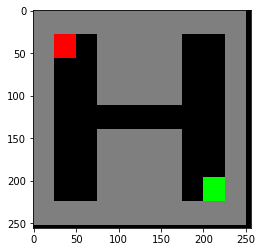
\includegraphics[width=0.3\linewidth]{figs/grid4.png}
    \caption{Environment 4 rendered from \textbf{a Github's implementation of the Distral paper}}
    \label{fig4.1}
\end{figure}
Furthermore, the original paper states that each state consists of the agent's current location, action and reward from the previous time step.\\

The original paper then compared the following algorithms:
\begin{itemize}
    \item distral trained using only KL reg and optimization algorithm that alternates between soft Q-learning and policy distillation, with each soft Q-learning iteration using rollout length 10 (n-step TD learning where n = 10)
    \item Distral agent to SQL that learns separate policy for each task.
\end{itemize}
\textbf{We will focus on the comparing the Distral algorithms with SQL or regularized Actor-Critic depending on the framework of Distral algorithms.} The complete list of available environments (fig \ref{fig:gridworlds}) is attached in the appendix. This report will mainly focus on environments 4, 5, 6, 7 and 8, as they are identical to the grid world presented in the original work.

\section{Experiments under SQL framework}
In this section we will compare the performance of Distral 1 col versus SQL and Distral 2 col versus SQL in different versions of the maze environment as demonstrated in  \cite{teh2017distral}. Both Distral algorithms will be implemented under the SQL framework as demonstrated in the pseudocode for algorithm \ref{alg:dist1colSQL}.

\subsection{Reproducing results from original work}

In the original work, Distral 2 cols via SQL was tested with $\alpha = 0$. That is, only the KL divergence penalty was included in the rewards. In addition, each SQL iteration uses a 10 step TD learning. The average rewards across tasks were then plotted as shown below
\begin{figure}[H]
    \center
    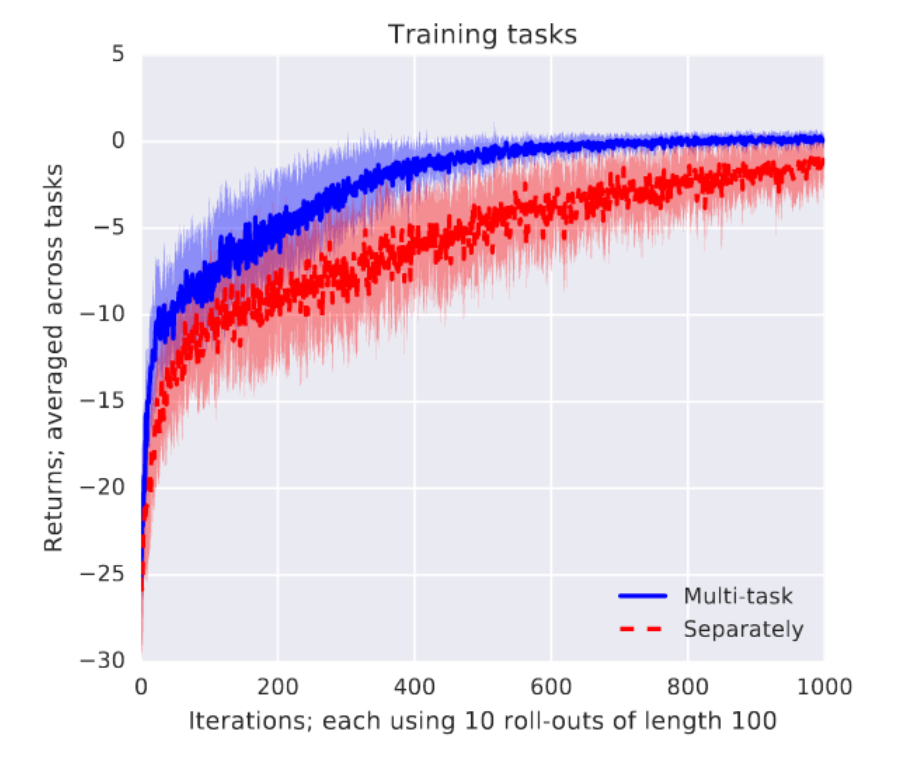
\includegraphics[width=0.5\linewidth]{figs/Distral_paper_res.png}
    \caption{Distral 2 col's original results for GridWorld}
\end{figure}
As shown above, Teh et al. \cite{teh2017distral} demonstrates Distral's ability to learn faster than training SQL on each task separately. Since it was not mentioned in the original work, we will use a simple 3 layer feedforward neural network with ReLU as the activation functions as function approximations of the policies, state and action value estimates.\\

This result is compared to this report's replication of the experiment
\begin{figure}[H]
\centering
\begin{minipage}{.5\textwidth}
\centering
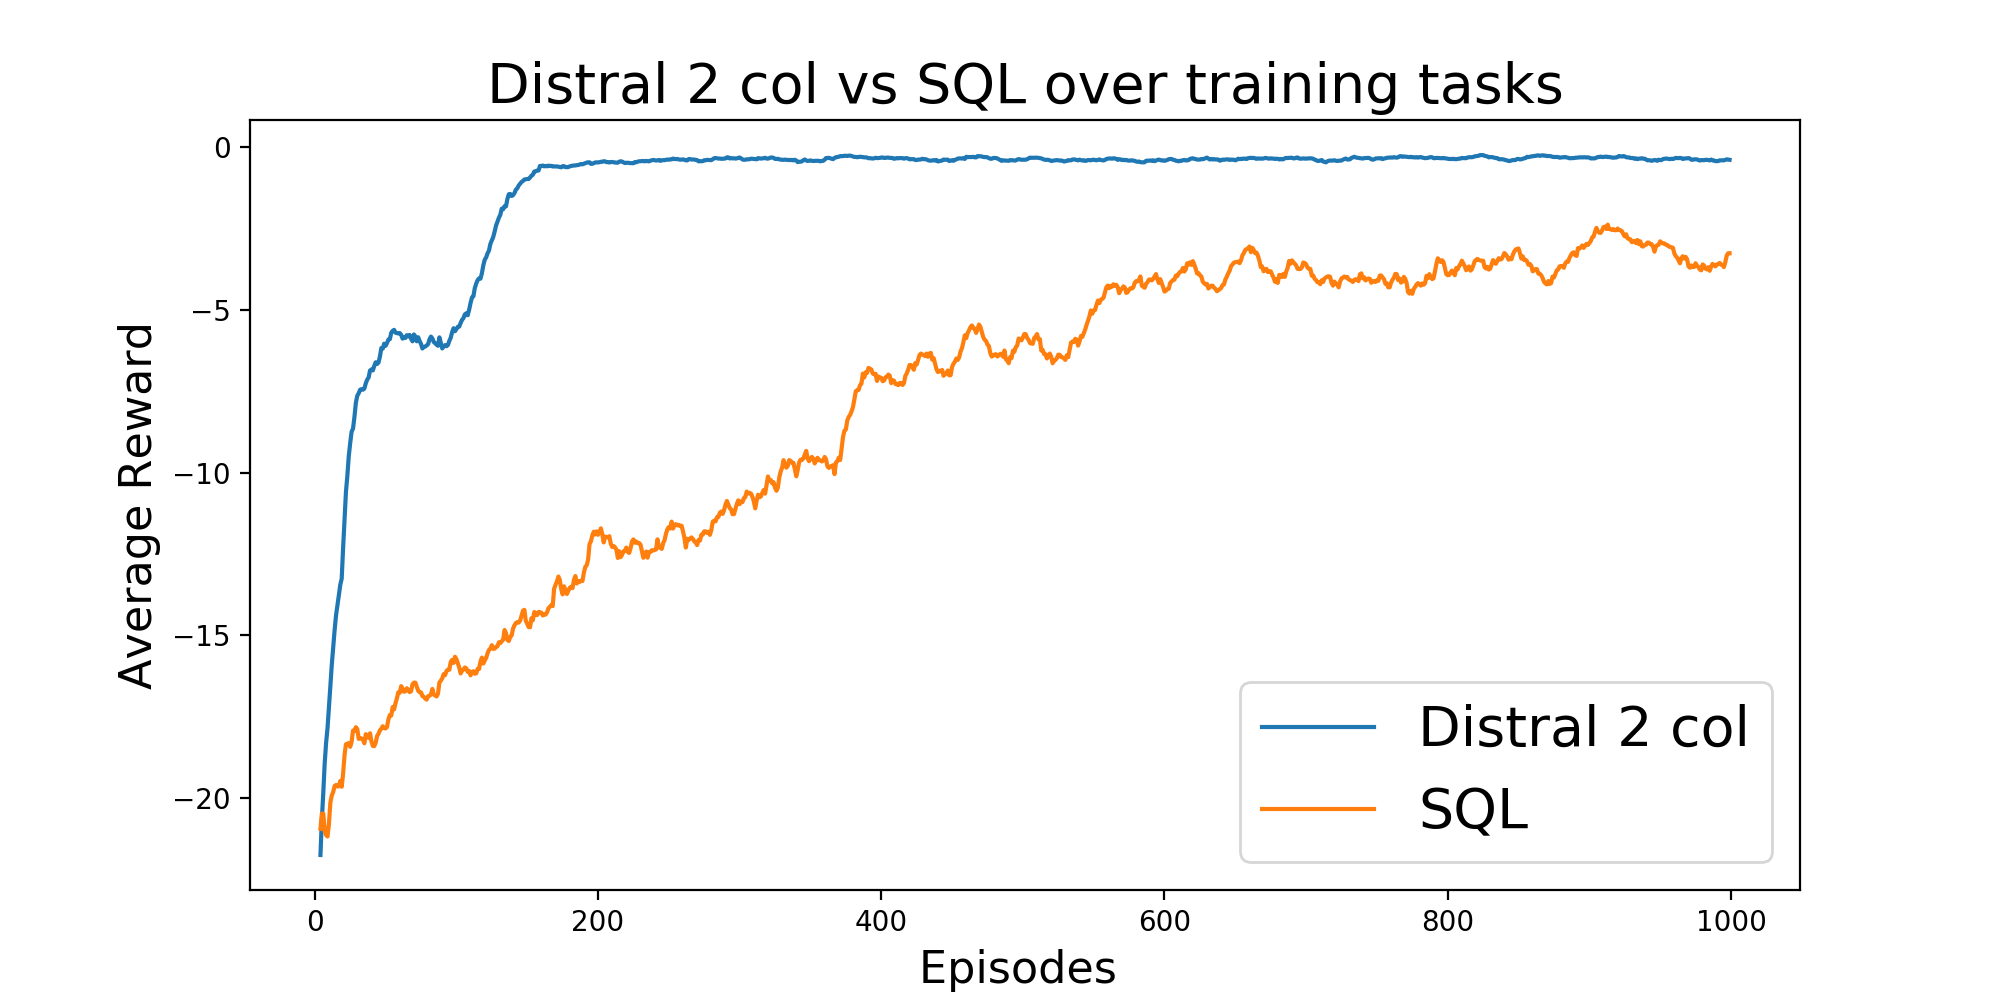
\includegraphics[width=\textwidth]{figs/distral_2_col_SQL_avg_rwd.png}
\end{minipage}%
\centering
\begin{minipage}{.5\textwidth}
\centering
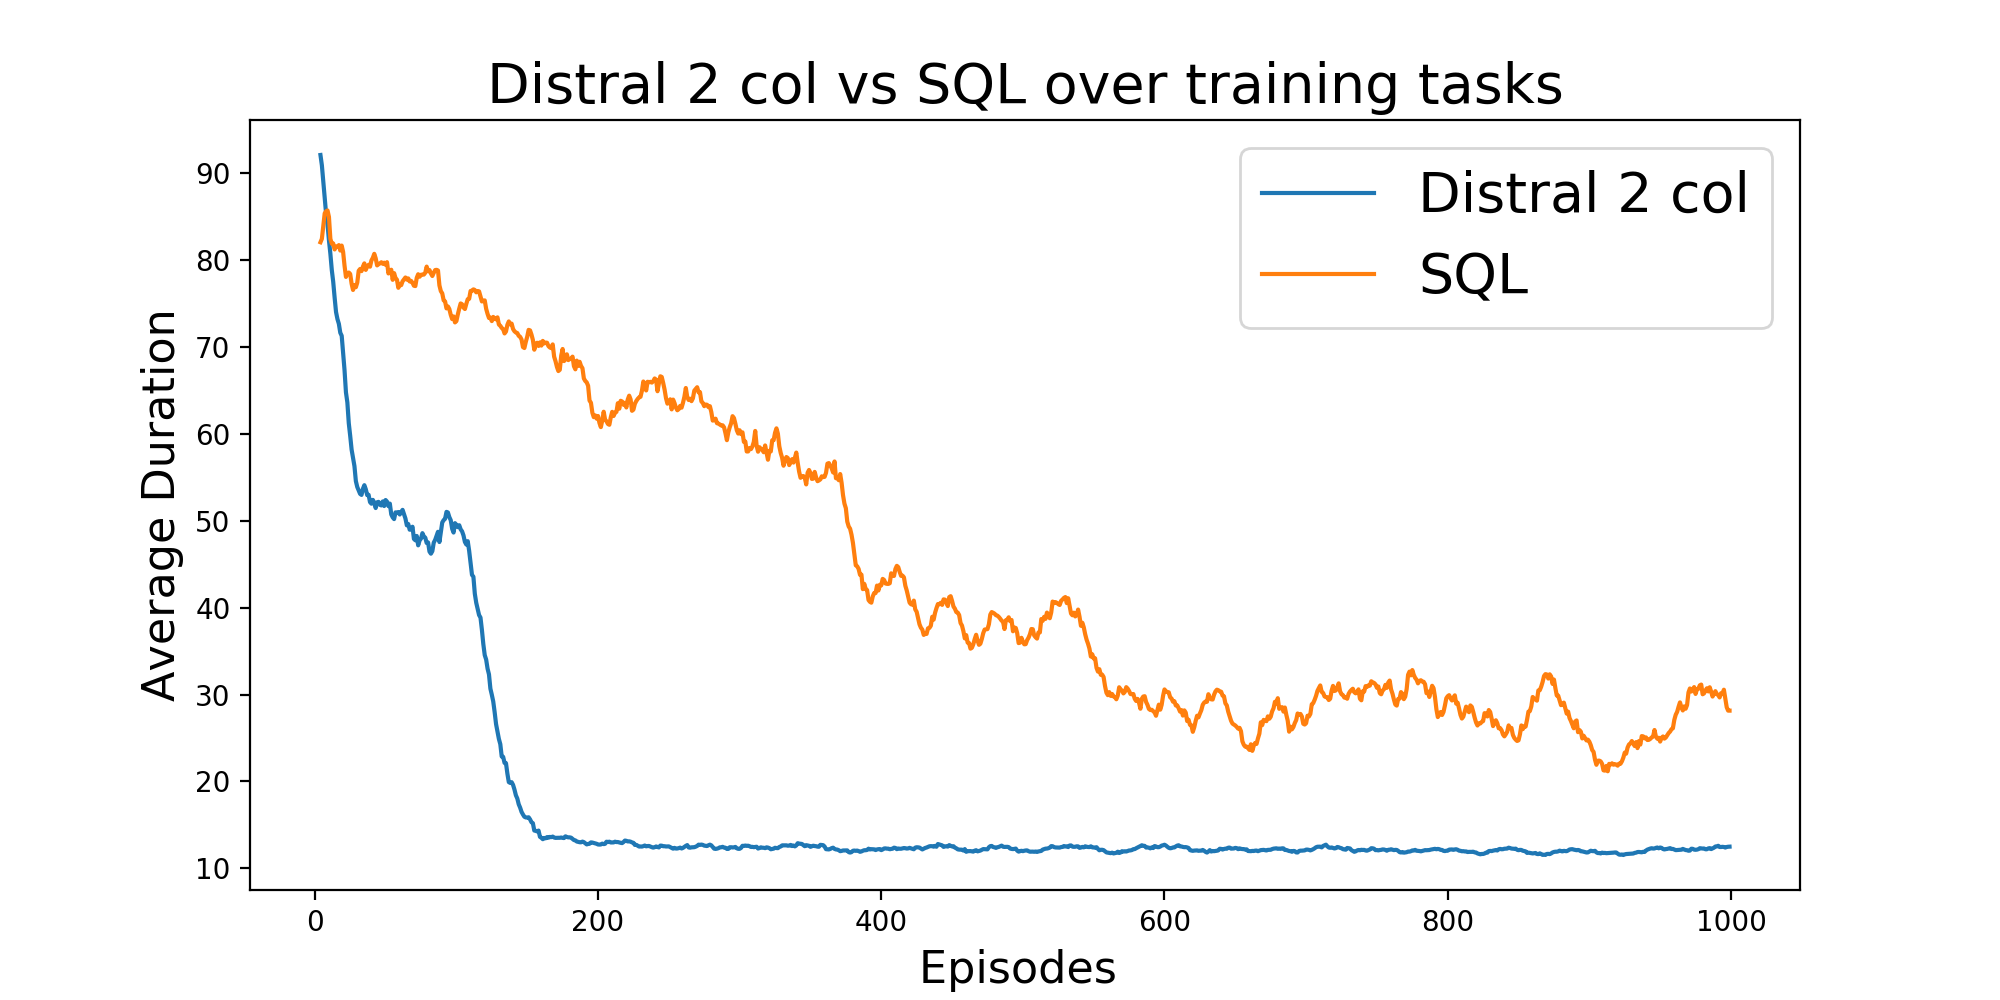
\includegraphics[width=\textwidth]{figs/distral_2_col_SQL_avg_dur.png}
\end{minipage}%
\end{figure}
As shown above, the results matches the behaviour demonstrated in the original paper. Distral 2 col via SQL learns significantly faster and has lower averaged duration and higher rewards across 5 tasks in the 2-corridor environment. Note that performance may vary depending on the architecture of the neural networks used in to approximate policies, state and action value estimates.

\subsection{Distral 1 col vs SQL}

Although the intended results are replicated through 10-step TD learning and setting the maximum number of episodes to 100, we should note that it is substantially more time consuming to conduct the experiments with such settings. Therefore, we will set $n=1$ instead of $n=10$ and maximum number of steps per episode to 1000 instead of 100. Given these new settings, we will also reduce the number of episodes from 1000 to 200 as one would expect the algorithms to converge quicker if the maximum number of steps per episode is increased by 10 folds. Below are the results of Distral 1 col via the SQL framework, versus SQL trained separately on each task.

\subsubsection{Environment 4 and 5}
\begin{figure}[H]
\centering
\begin{minipage}{.5\textwidth}
\centering
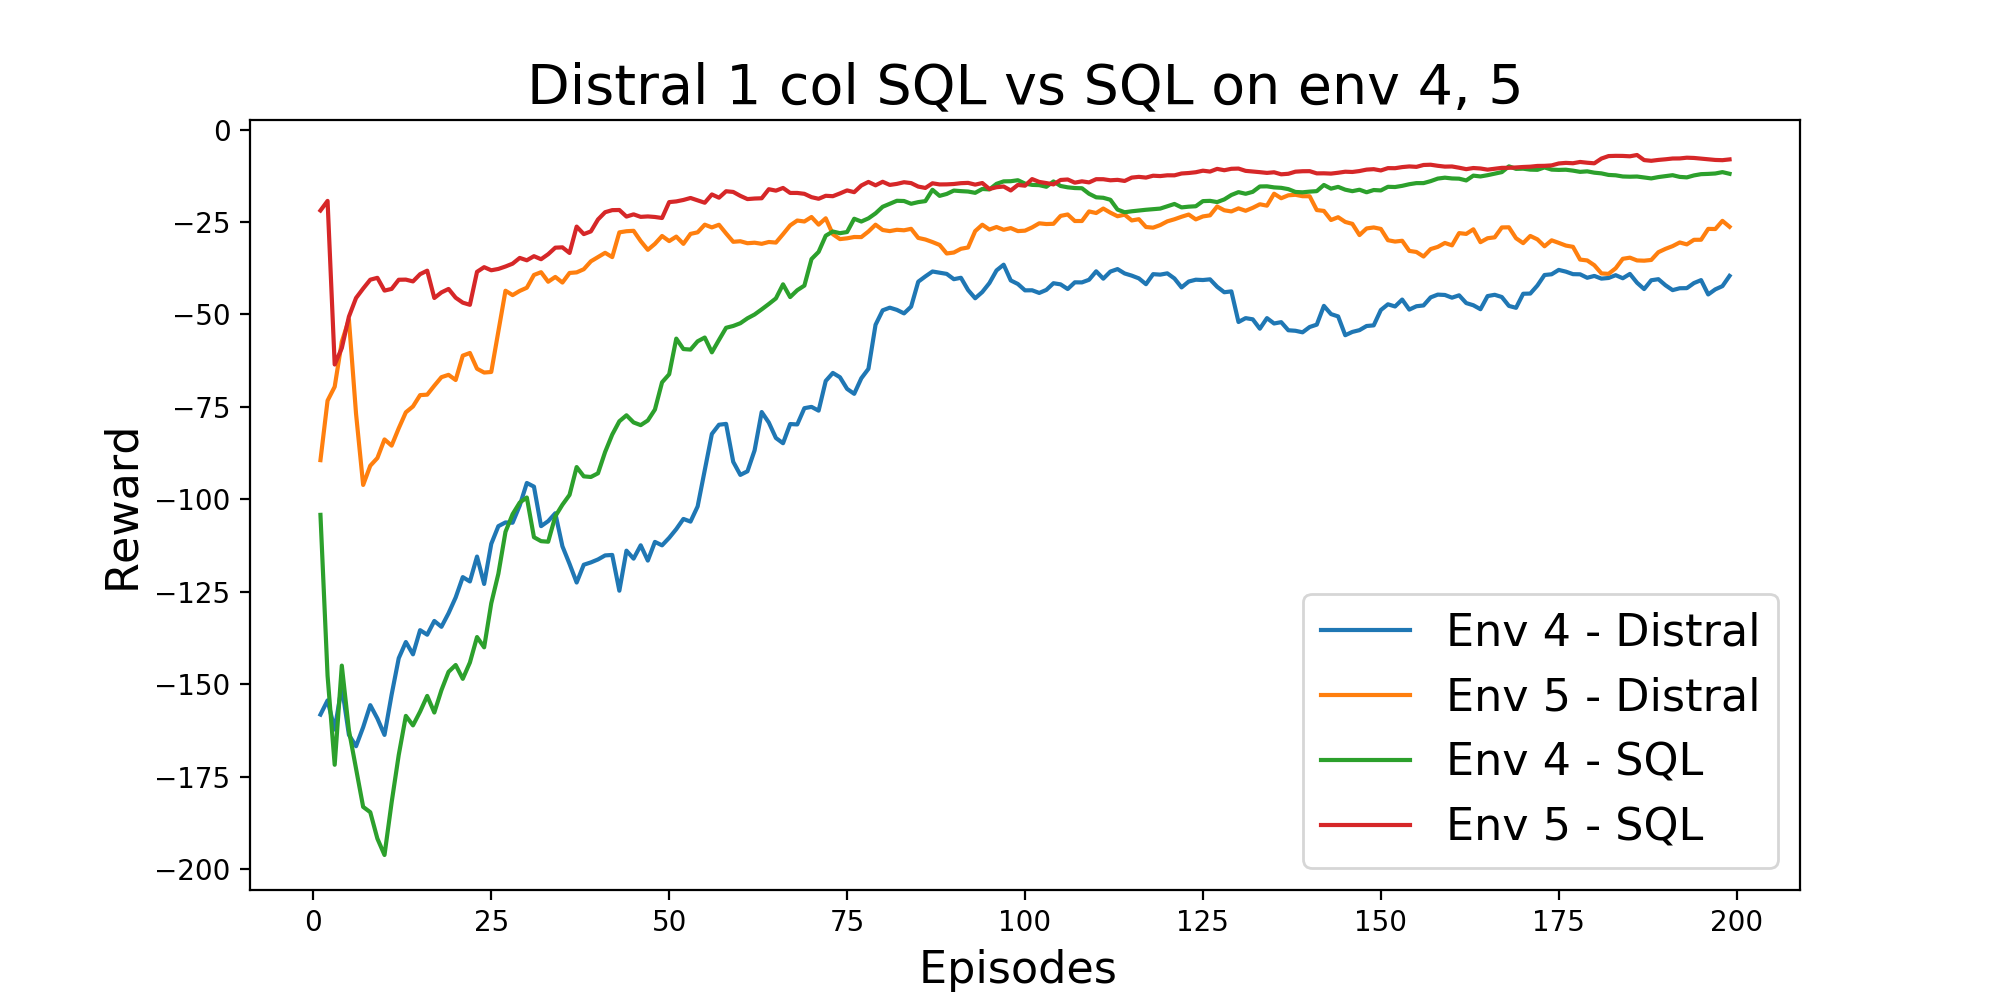
\includegraphics[width=\textwidth]{figs/d1_col_sql/d1_col_sql_4_5_rwd.png}
\end{minipage}%
\centering
\begin{minipage}{.5\textwidth}
\centering
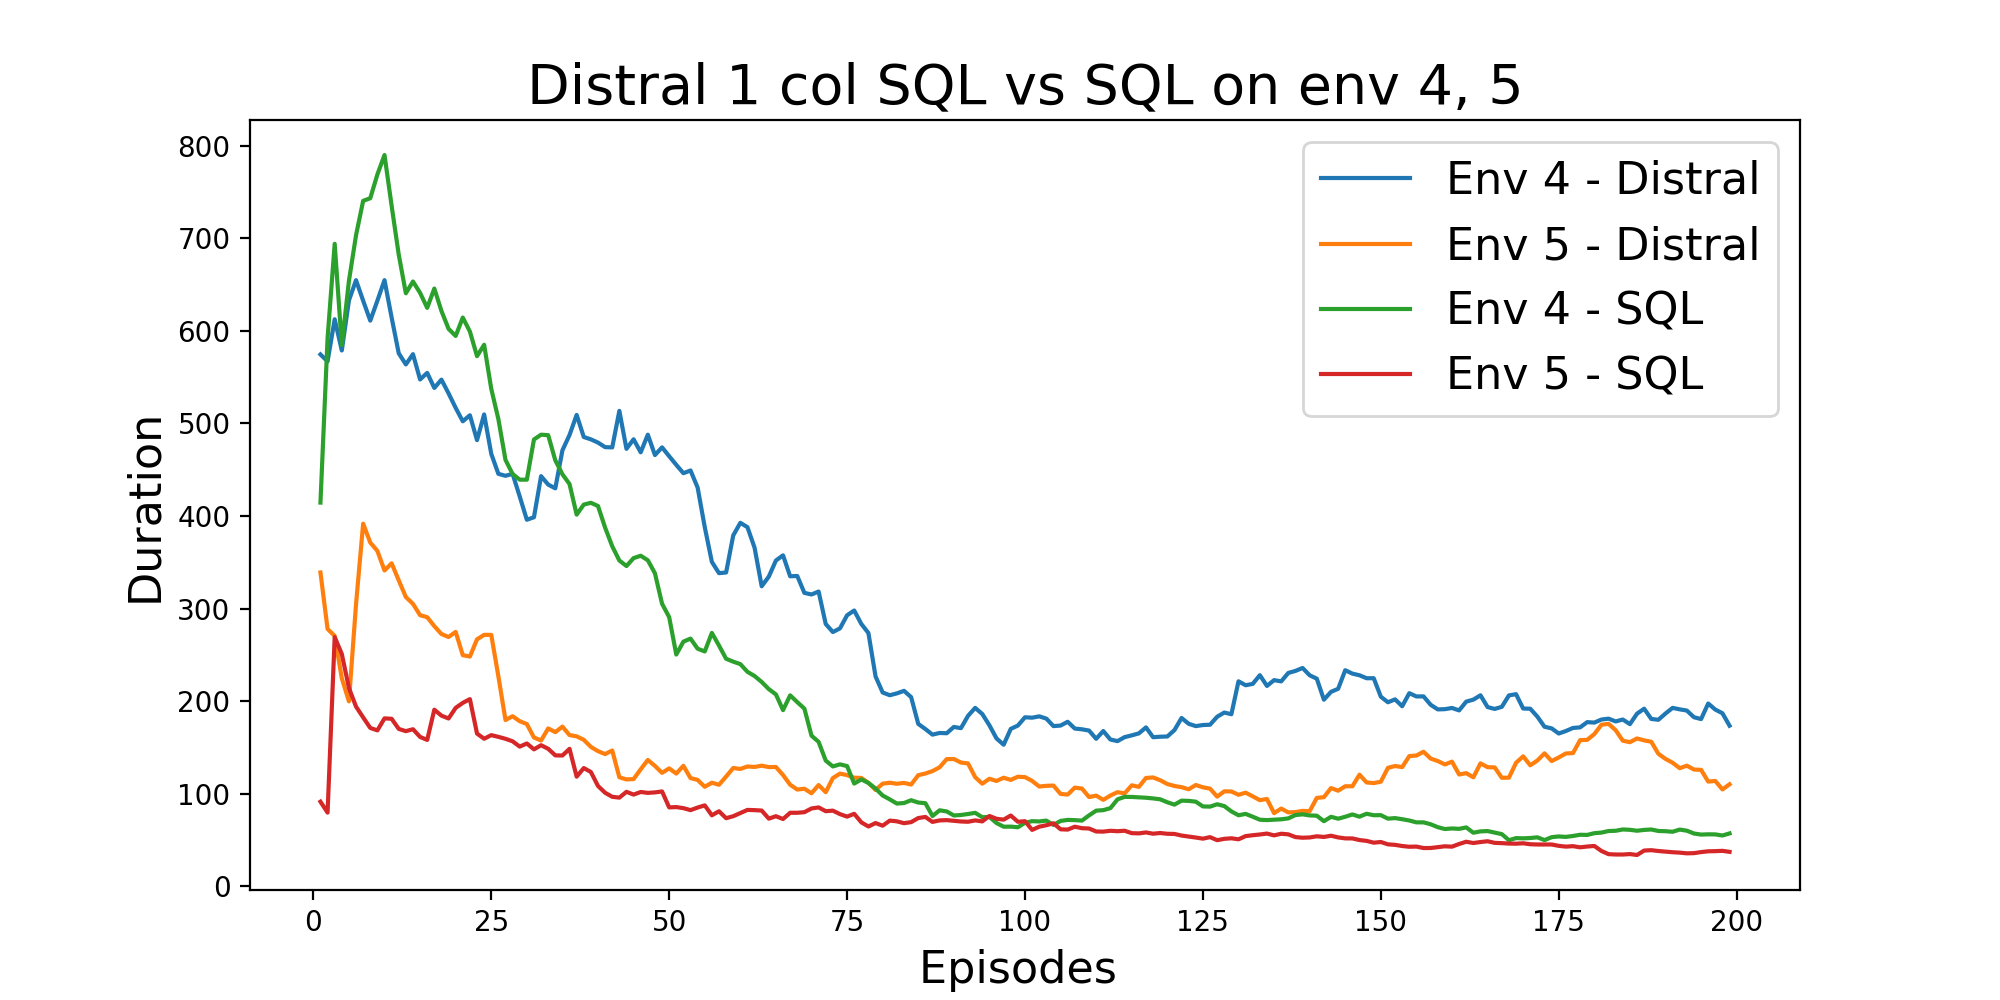
\includegraphics[width=\textwidth]{figs/d1_col_sql/d1_col_sql_4_5_dur.png}
\end{minipage}%
\end{figure}
Here we see that SQL is performing better than Distral 1 col, converging earlier and to a lower duration per episode. We also see that Distral 1 col has converged to a local optimum at around 100 steps for environment 4 and 80 steps for environment 5.

\subsubsection{Environment 7 and 8}
\begin{figure}[H]
\centering
\begin{minipage}{.5\textwidth}
\centering
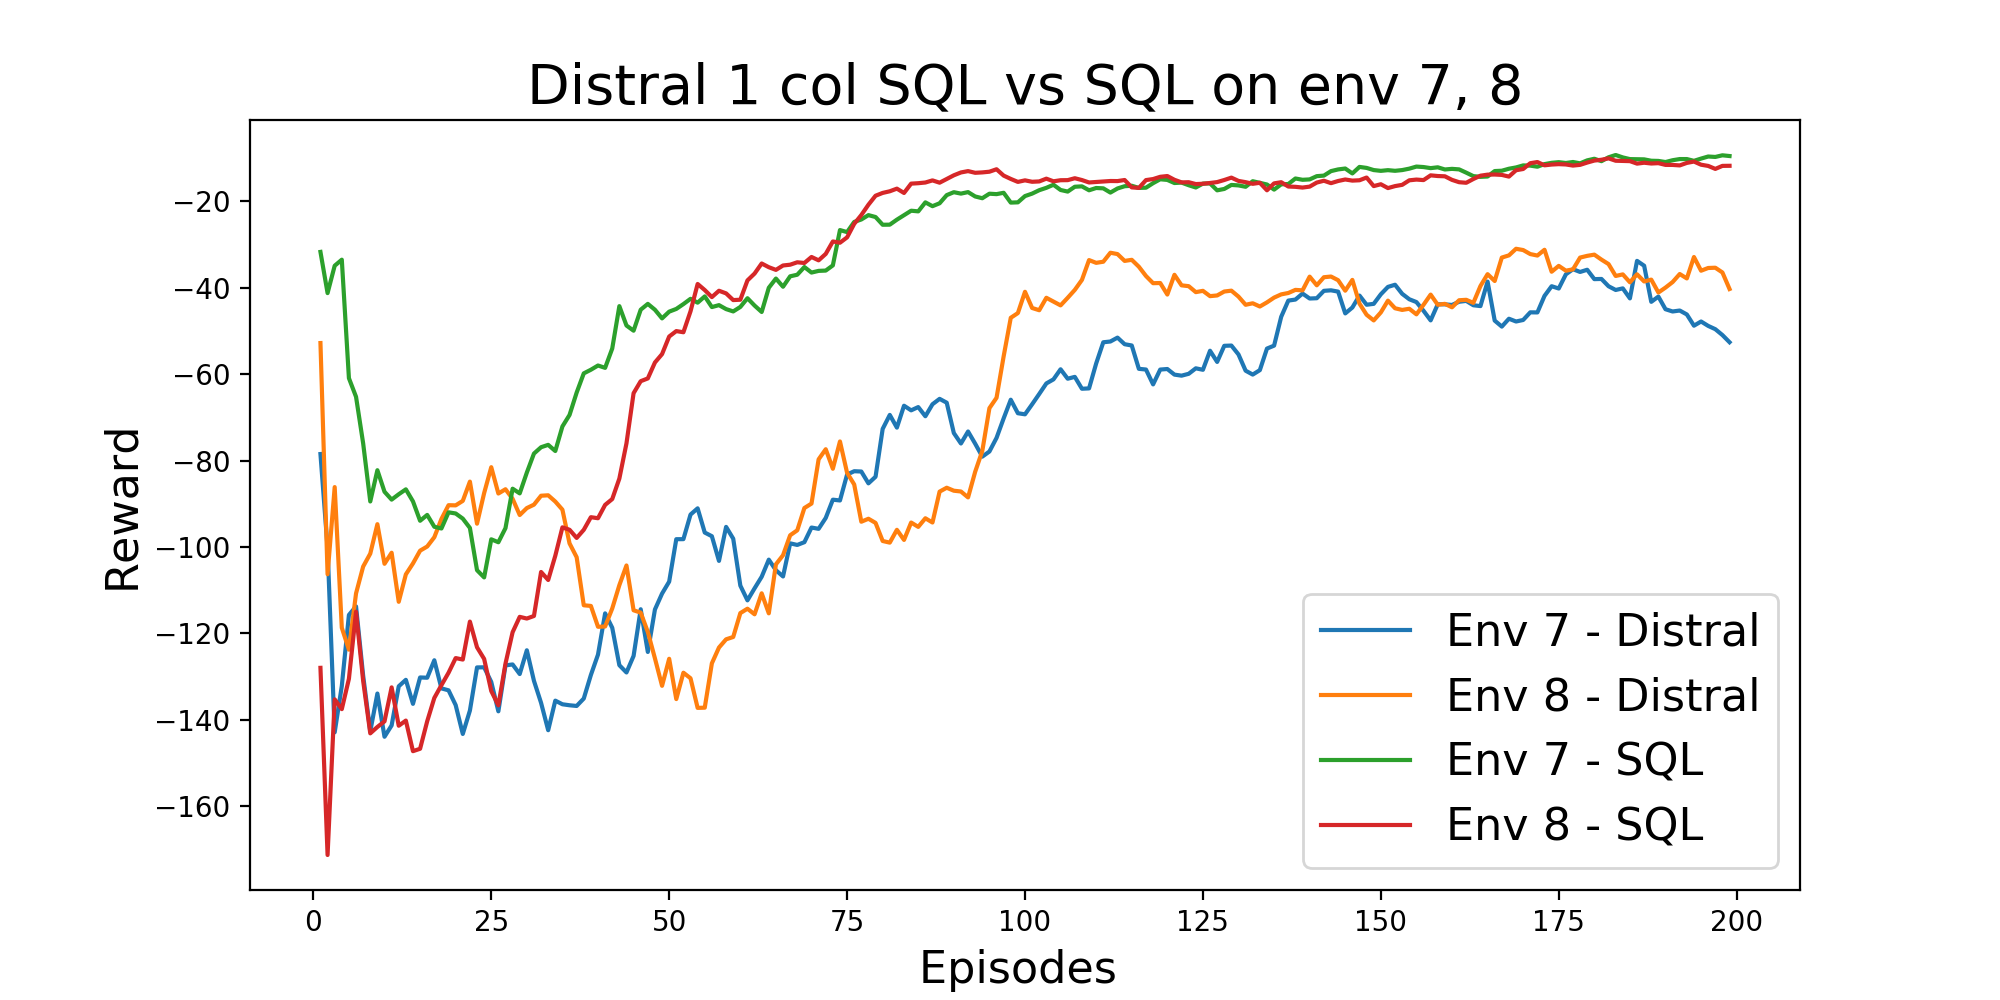
\includegraphics[width=\textwidth]{figs/d1_col_sql/d1_col_sql_7_8_rwd.png}
\end{minipage}%
\centering
\begin{minipage}{.5\textwidth}
\centering
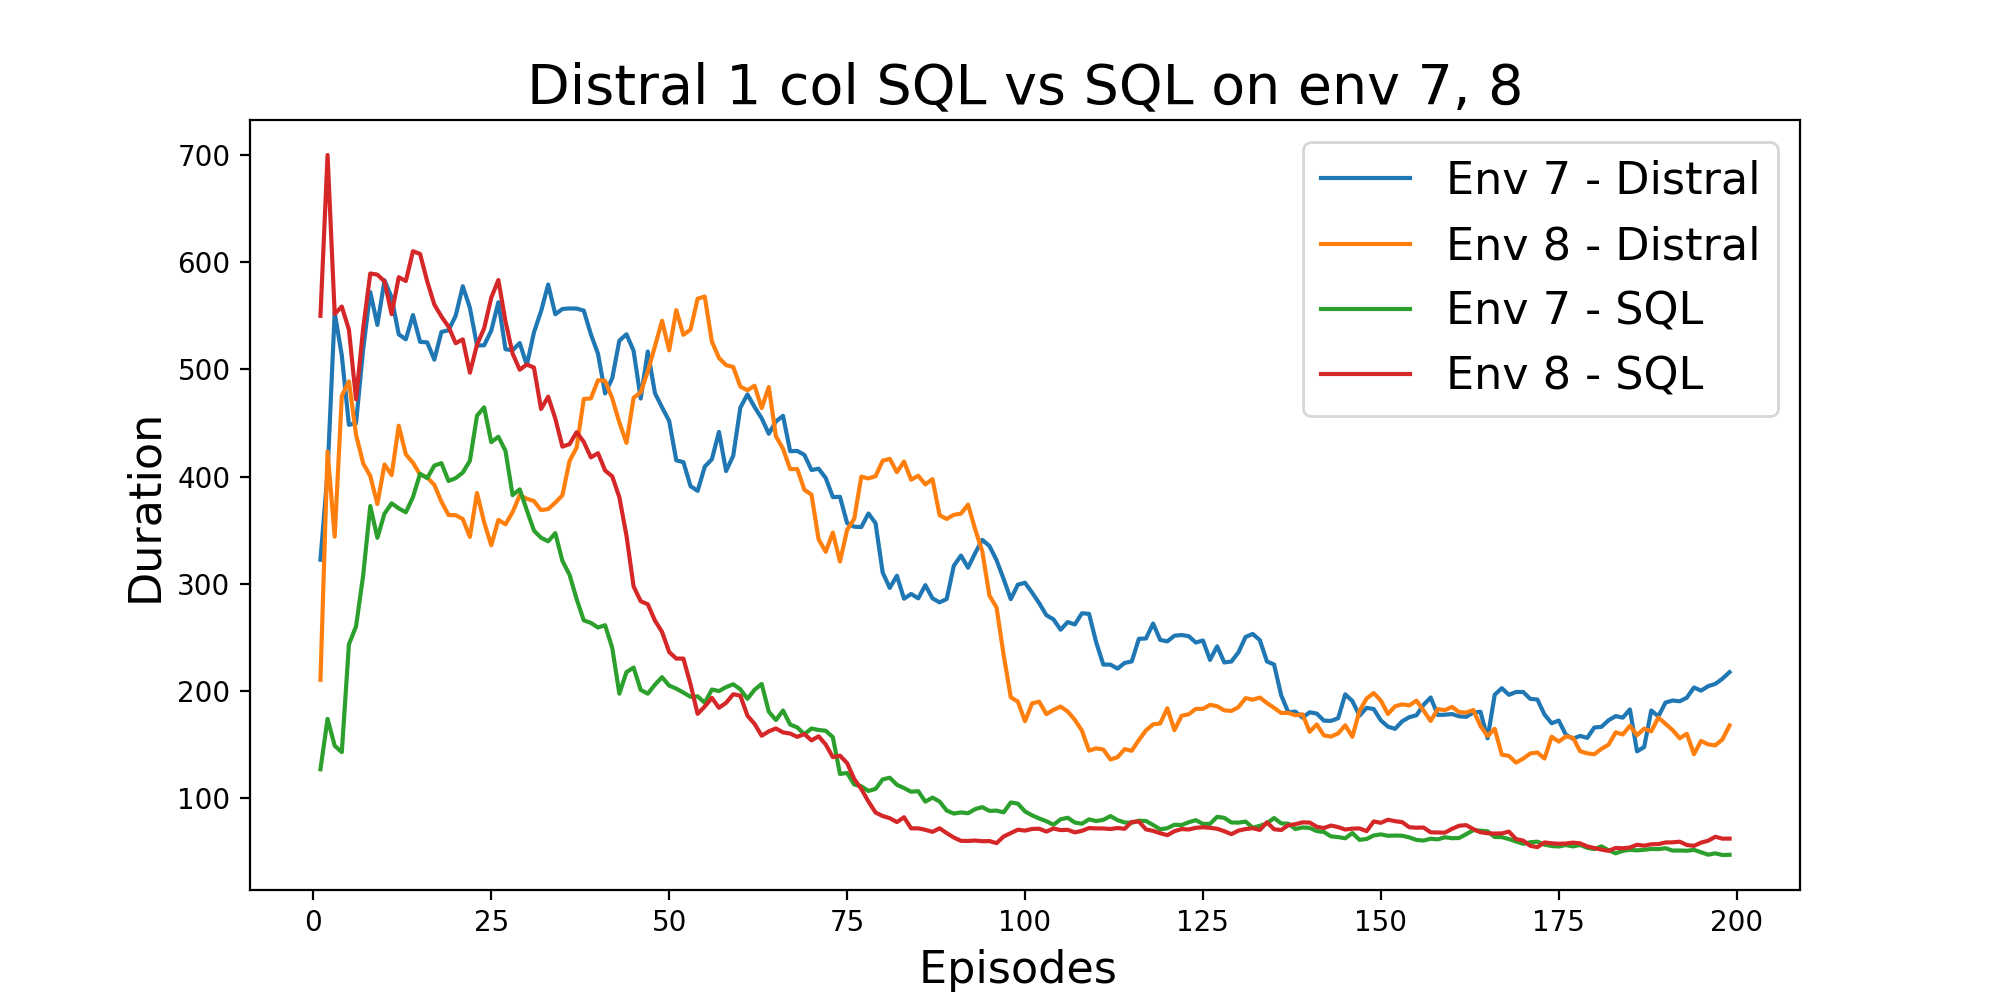
\includegraphics[width=\textwidth]{figs/d1_col_sql/d1_col_sql_7_8_dur.png}
\end{minipage}%
\end{figure}
Here we see that SQL is once again performing better than Distral 1 col in terms of both convergence and the duration it takes to reach the goal state.

\subsubsection{Environments 4, 5 and 7}
\begin{figure}[H]
\centering
\begin{minipage}{.5\textwidth}
\centering
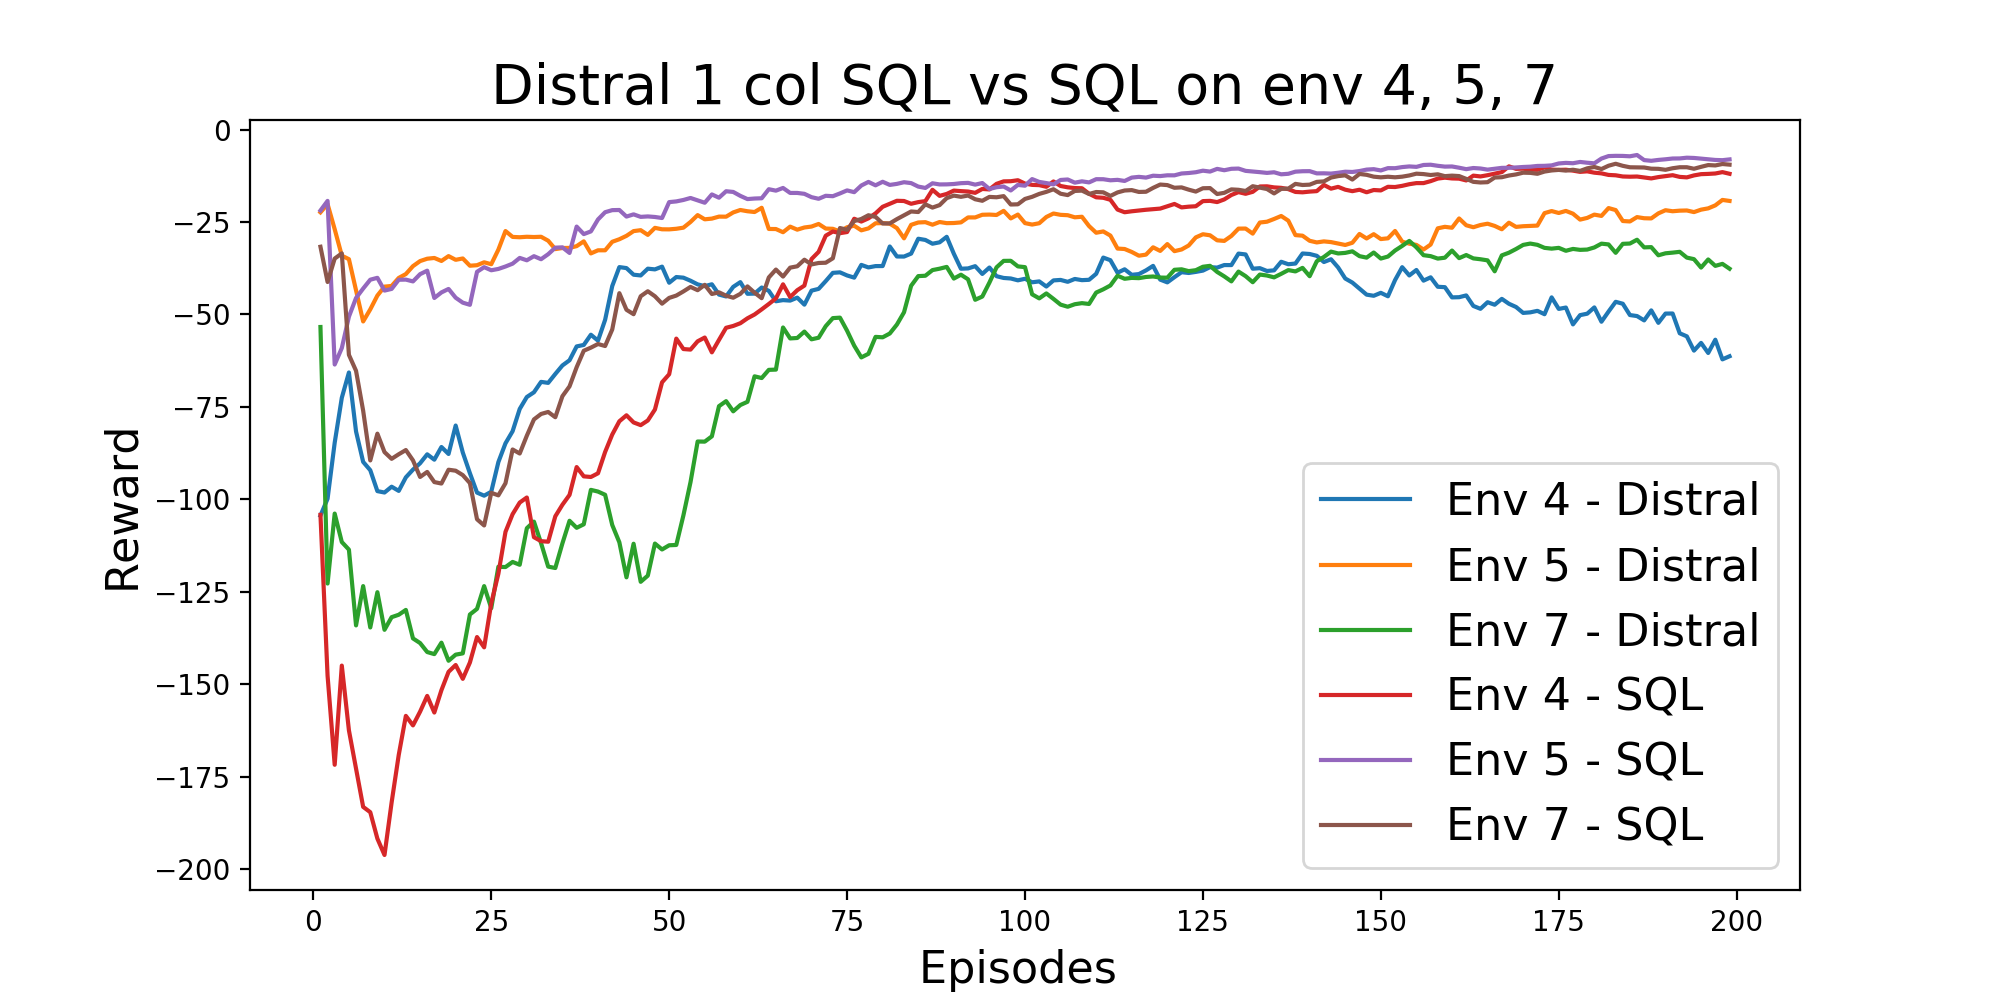
\includegraphics[width=\textwidth]{figs/d1_col_sql/d1_col_sql_4_5_7_rwd.png}
\end{minipage}%
\centering
\begin{minipage}{.5\textwidth}
\centering
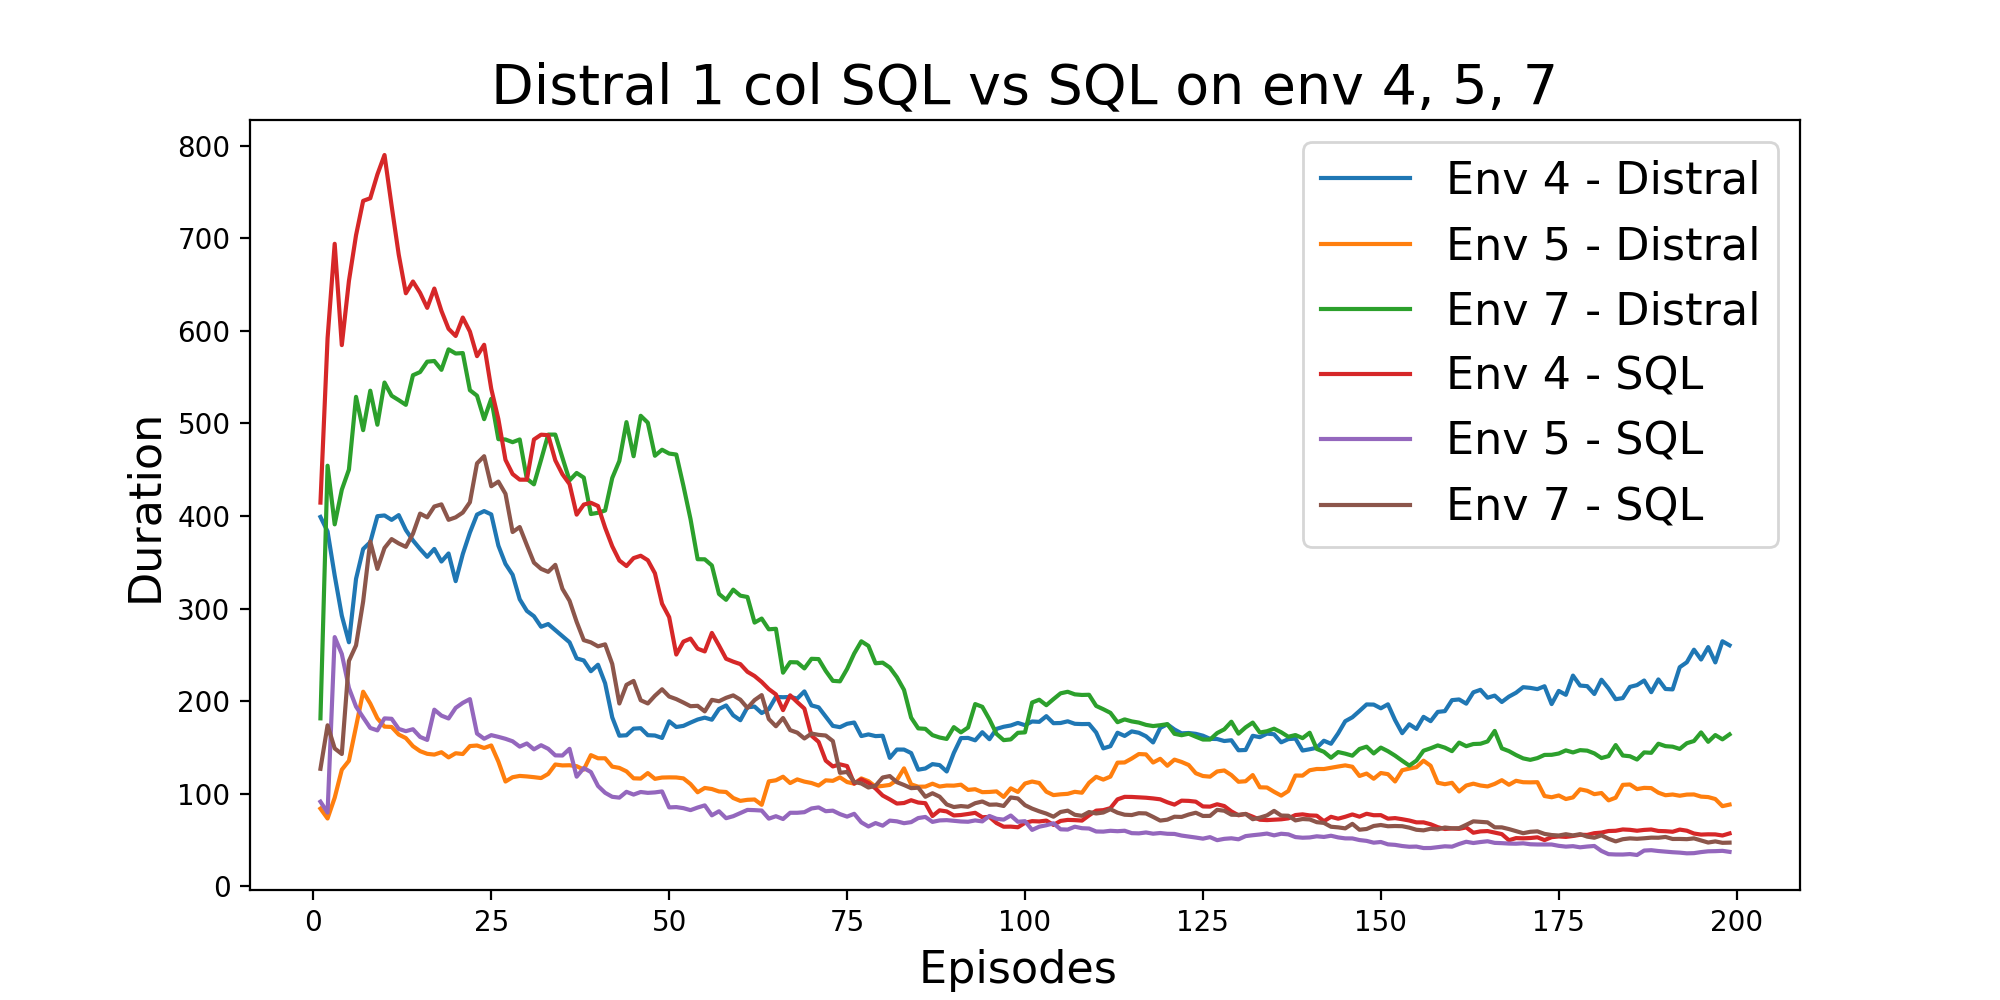
\includegraphics[width=\textwidth]{figs/d1_col_sql/d1_col_sql_4_5_7_dur.png}
\end{minipage}%
\end{figure}
Here we see that Distral 1 col is performing significantly worst than SQL. This suggests that Distral 1 col's performance becomes highly volatile when learning more than 2 environments. We should also note that environment 4 and 7 are "hard" in a sense that the distance it takes for the agent to traverse from start to goal state is the furthest among all testing environments.

\subsubsection{Environments 4, 5, 6, 7, 8}
\begin{figure}[H]
\centering
\begin{minipage}{.5\textwidth}
\centering
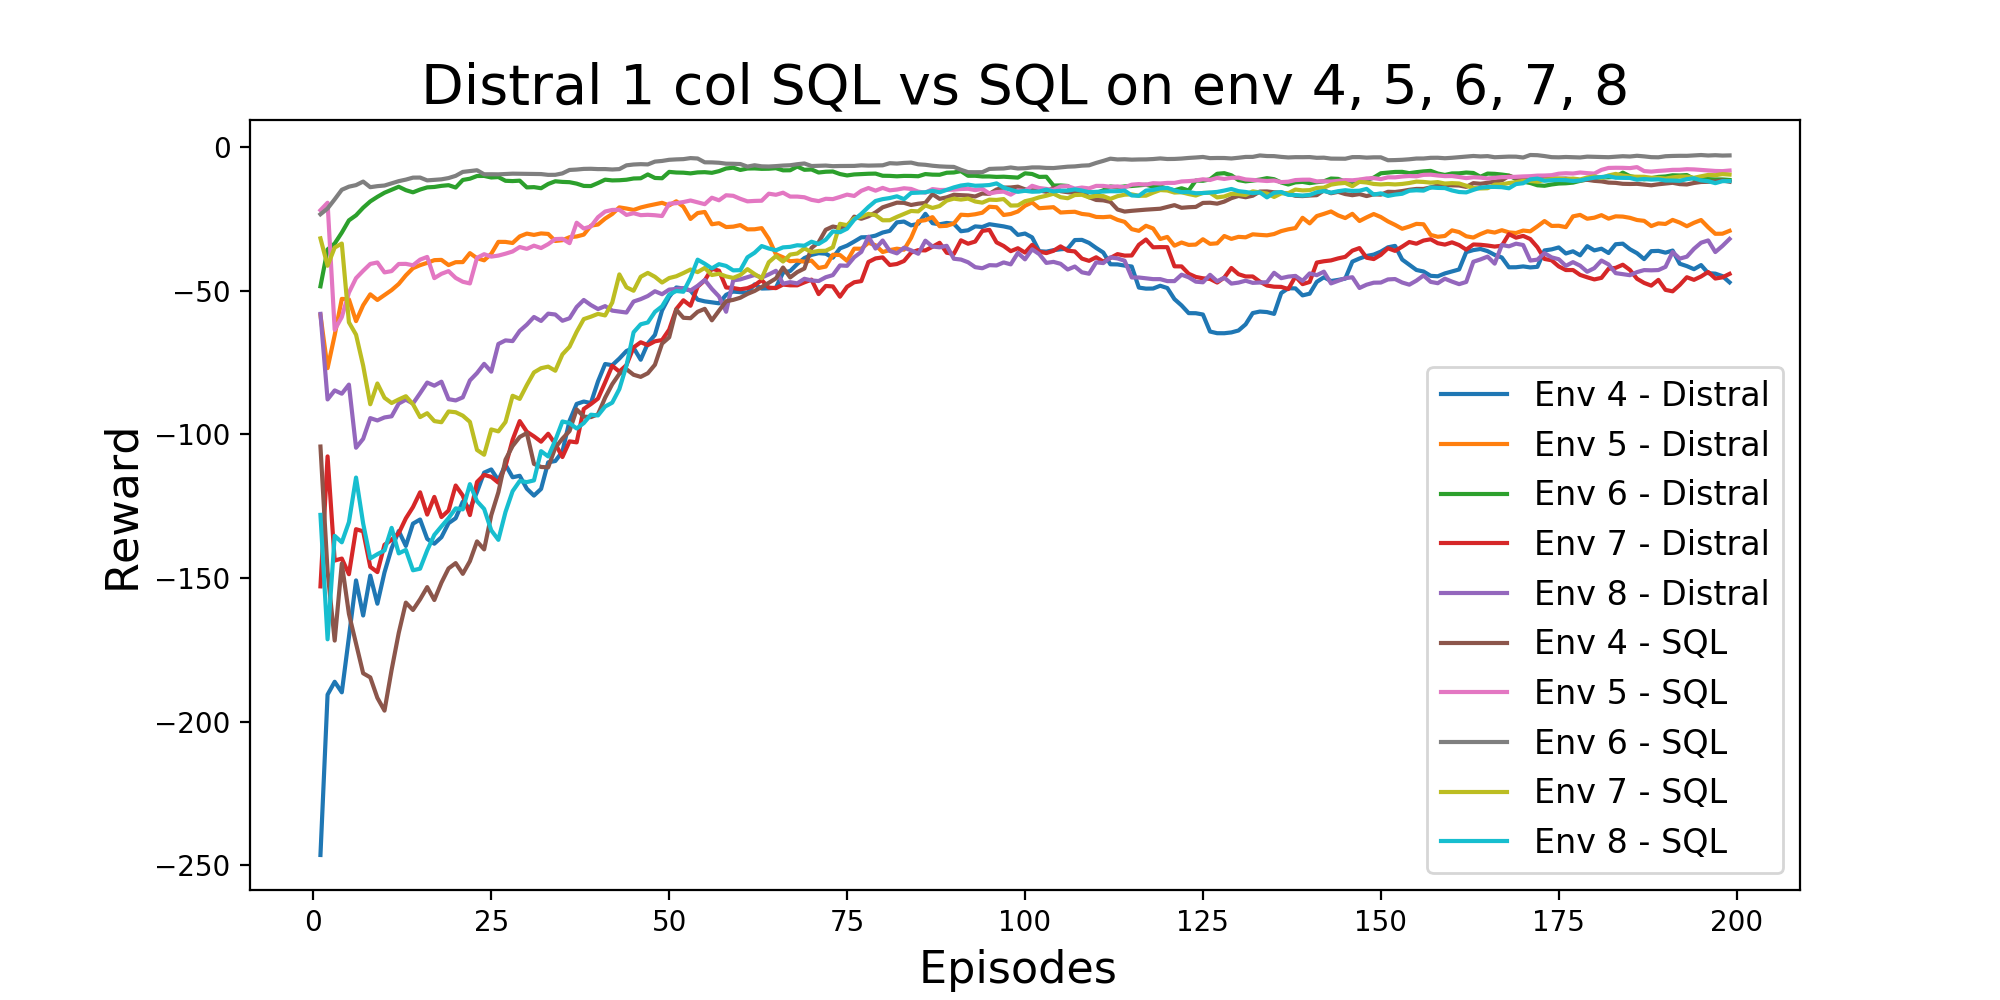
\includegraphics[width=\textwidth]{figs/d1_col_sql/d1_col_sql_4_5_6_7_8_rwd.png}
\end{minipage}%
\centering
\begin{minipage}{.5\textwidth}
\centering
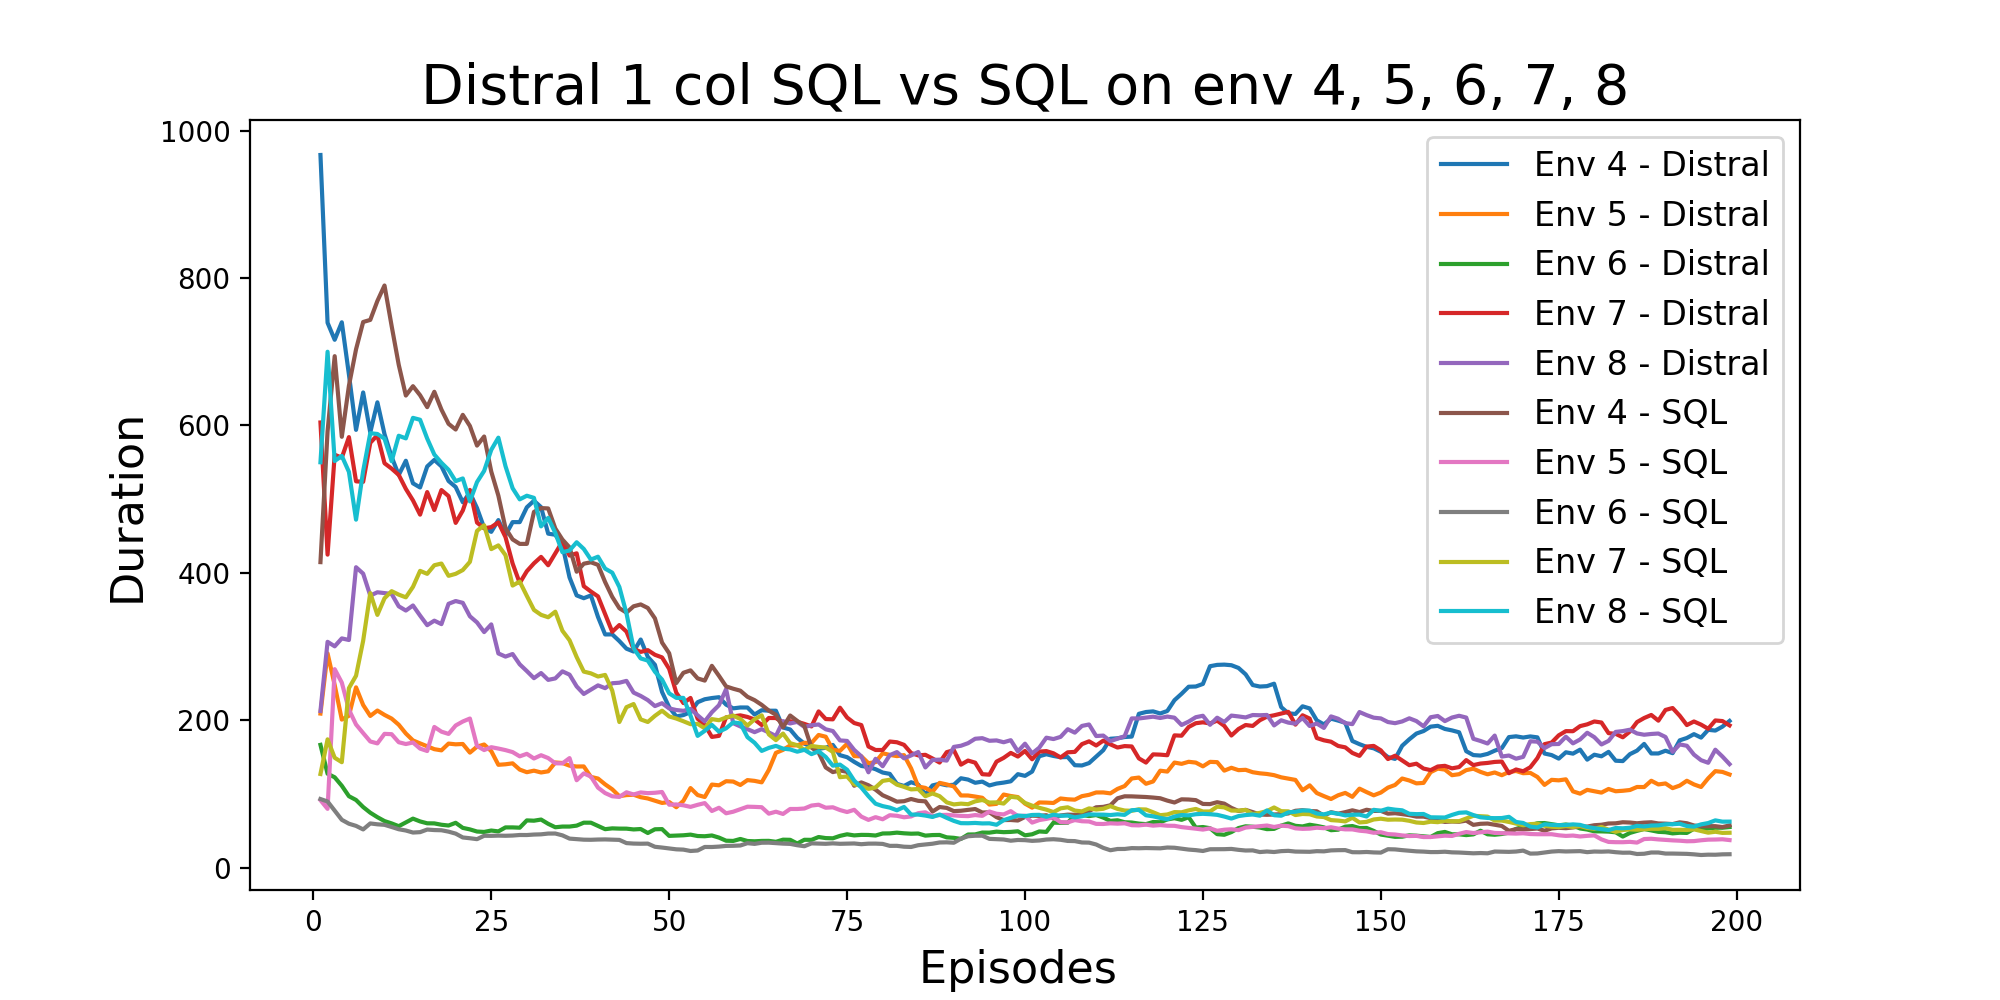
\includegraphics[width=\textwidth]{figs/d1_col_sql/d1_col_sql_4_5_6_7_8_dur.png}
\end{minipage}%
\end{figure}
As shown above, the duration for most tasks are around 200 steps, indicating Distral 1 col did not solve most of the environments when it is tasked to solve all 5 environments at the same time.

\subsection{Distral 2 col vs SQL}

Here are the benchmark results for training Distral 2 col under SQL framework versus SQL, with the same settings as mentioned in the previous subsection. Again, the Distral algorithm is conducted under the SQL framework and compared against SQL trained separately on each task.
\subsubsection{Environment 4 and 5}
\begin{figure}[H]
\centering
\begin{minipage}{.5\textwidth}
\centering
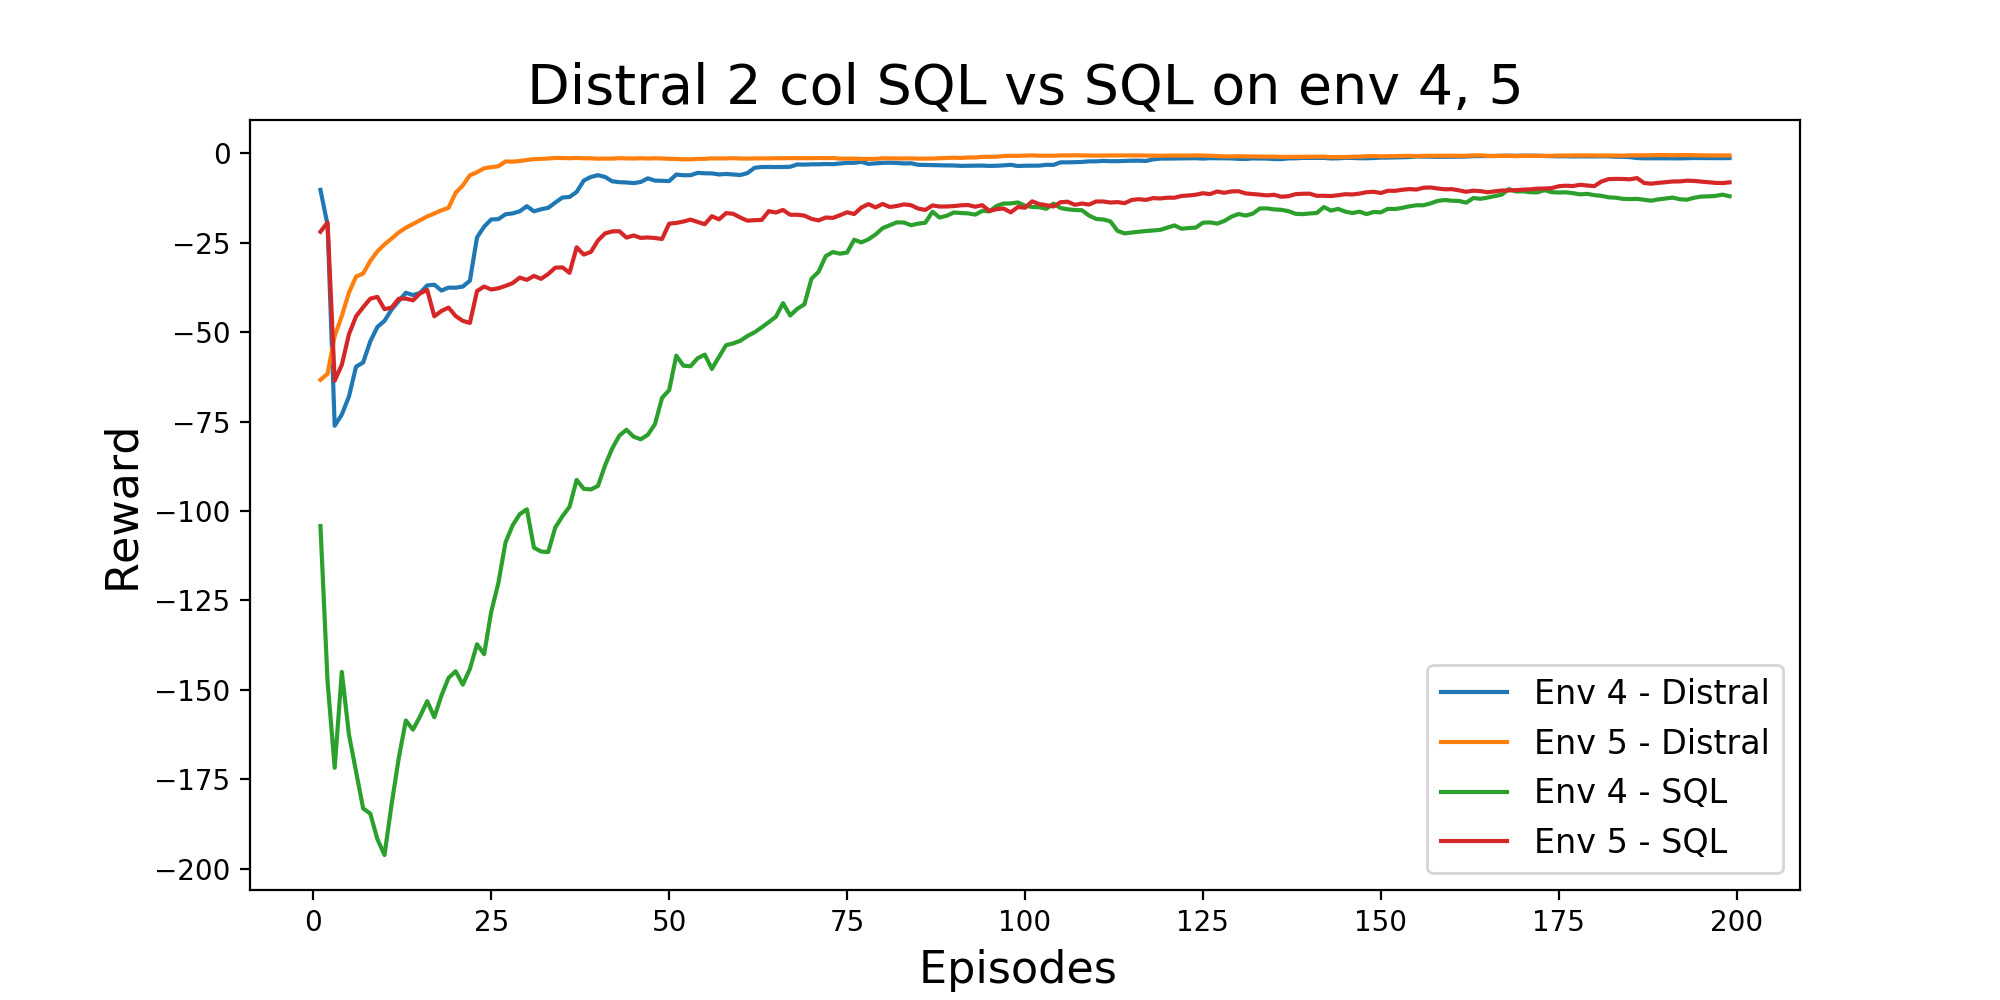
\includegraphics[width=\textwidth]{figs/d2_col_sql/d2_col_sql_4_5_rwd.png}
\end{minipage}%
\centering
\begin{minipage}{.5\textwidth}
\centering
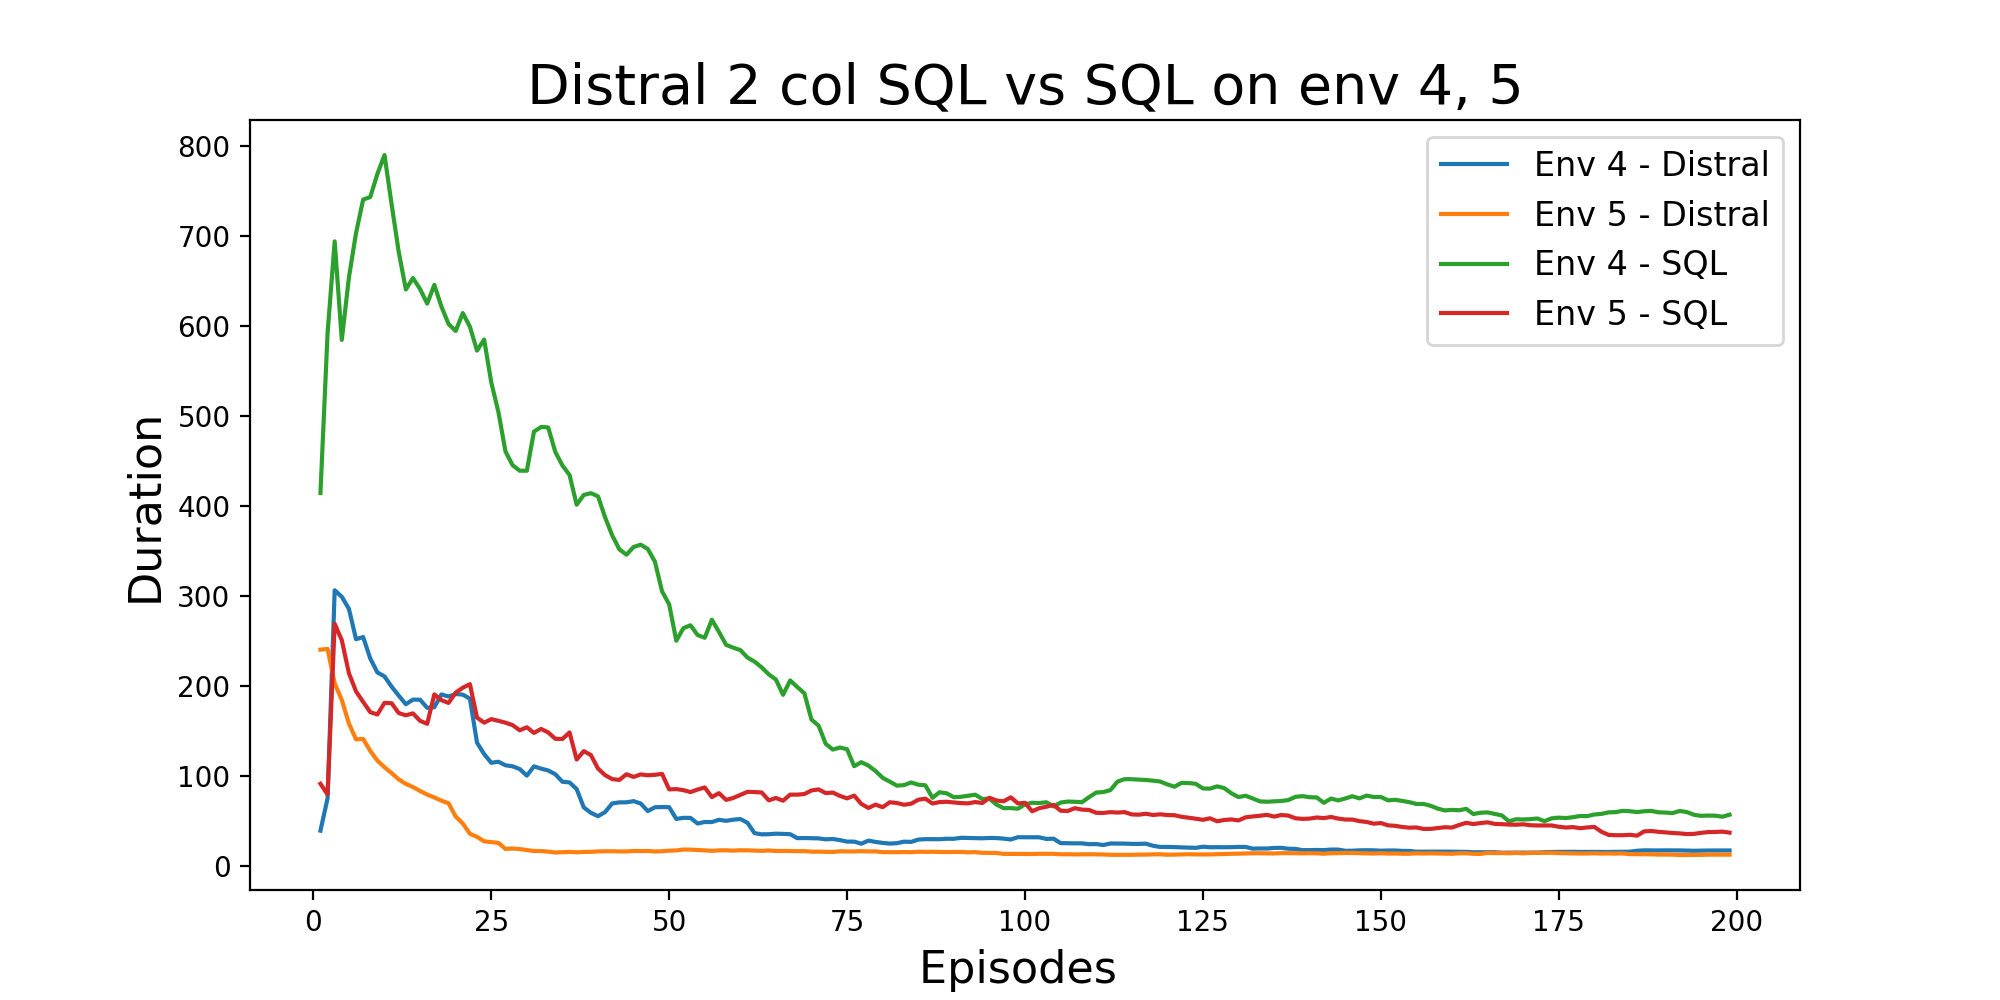
\includegraphics[width=\textwidth]{figs/d2_col_sql/d2_col_sql_4_5_dur.png}
\end{minipage}%
\end{figure}
The diagrams above shows a significant difference in performance between Distral 1 col and 2 col. Here we see that Distral 2 col converged much faster than Distral 1 col did and significantly outperforms the SQL baseline.
\subsubsection{Environment 7 and 8}
\begin{figure}[H]
\centering
\begin{minipage}{.5\textwidth}
\centering
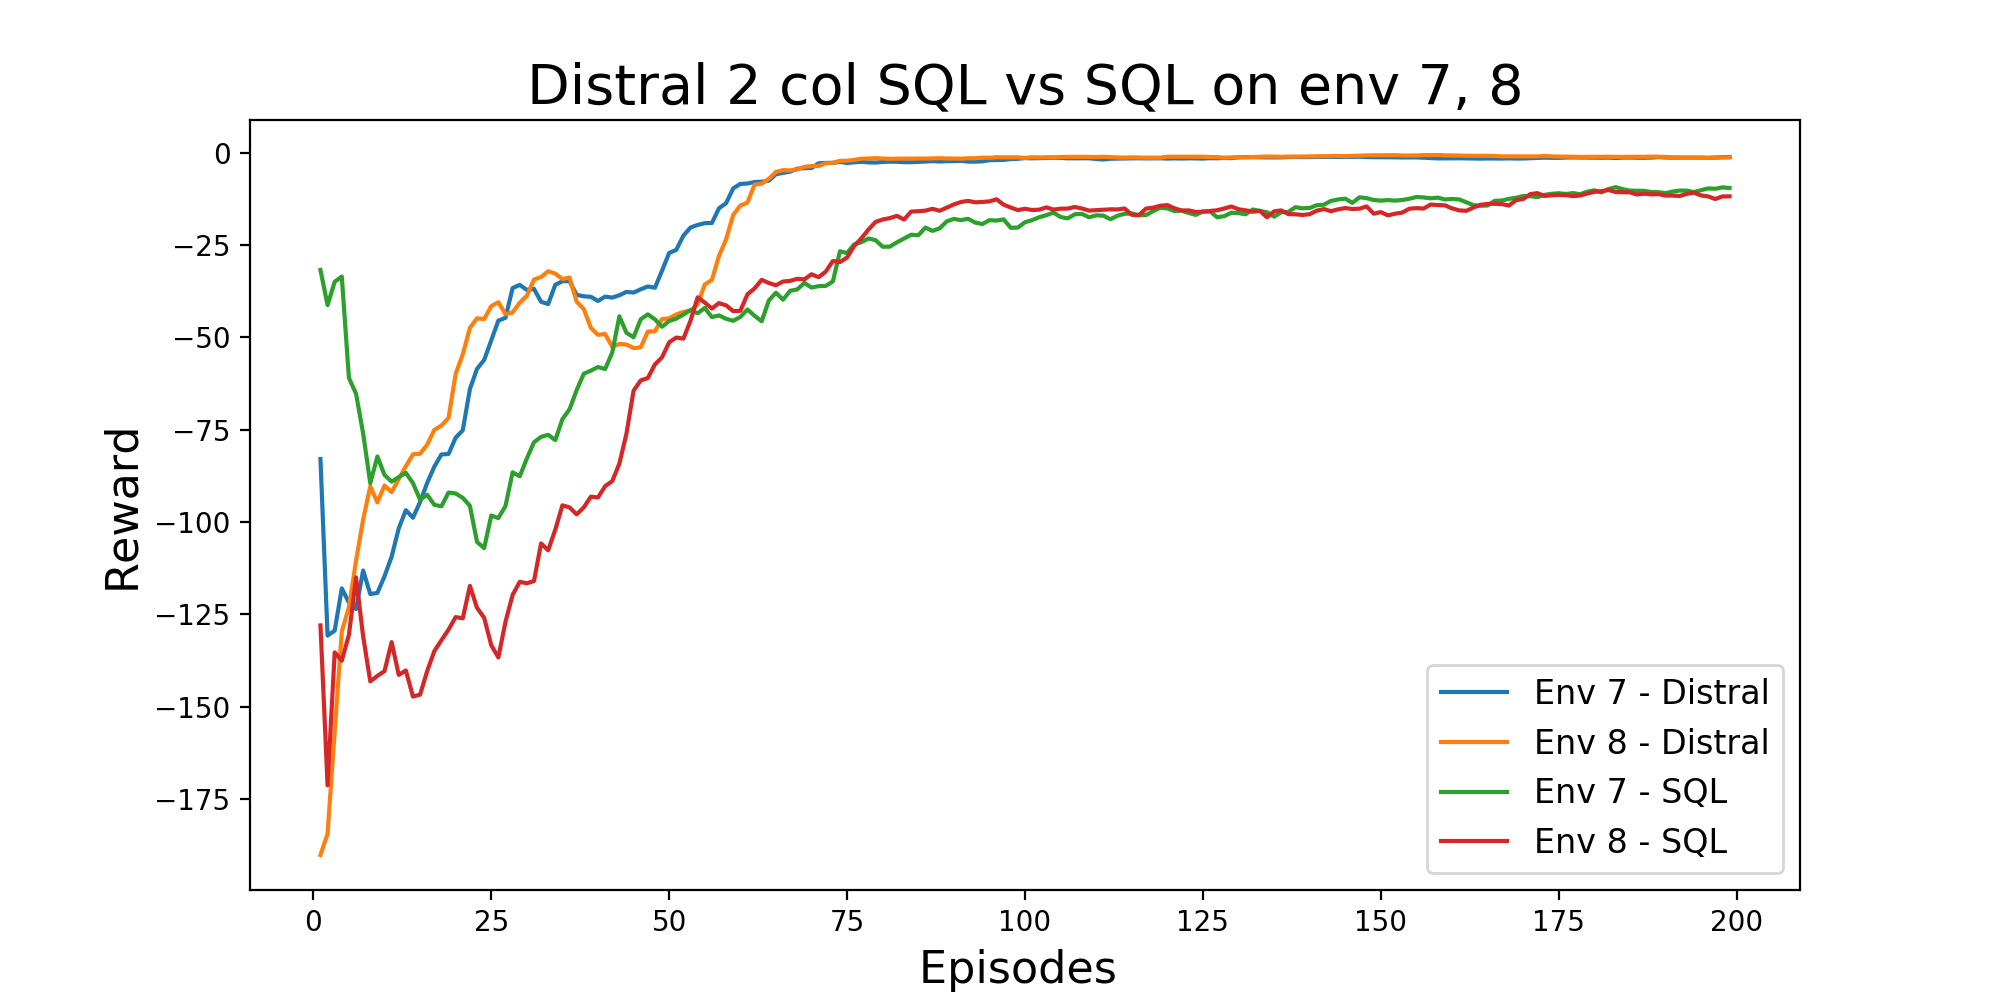
\includegraphics[width=\textwidth]{figs/d2_col_sql/d2_col_sql_7_8_rwd.png}
\end{minipage}%
\centering
\begin{minipage}{.5\textwidth}
\centering
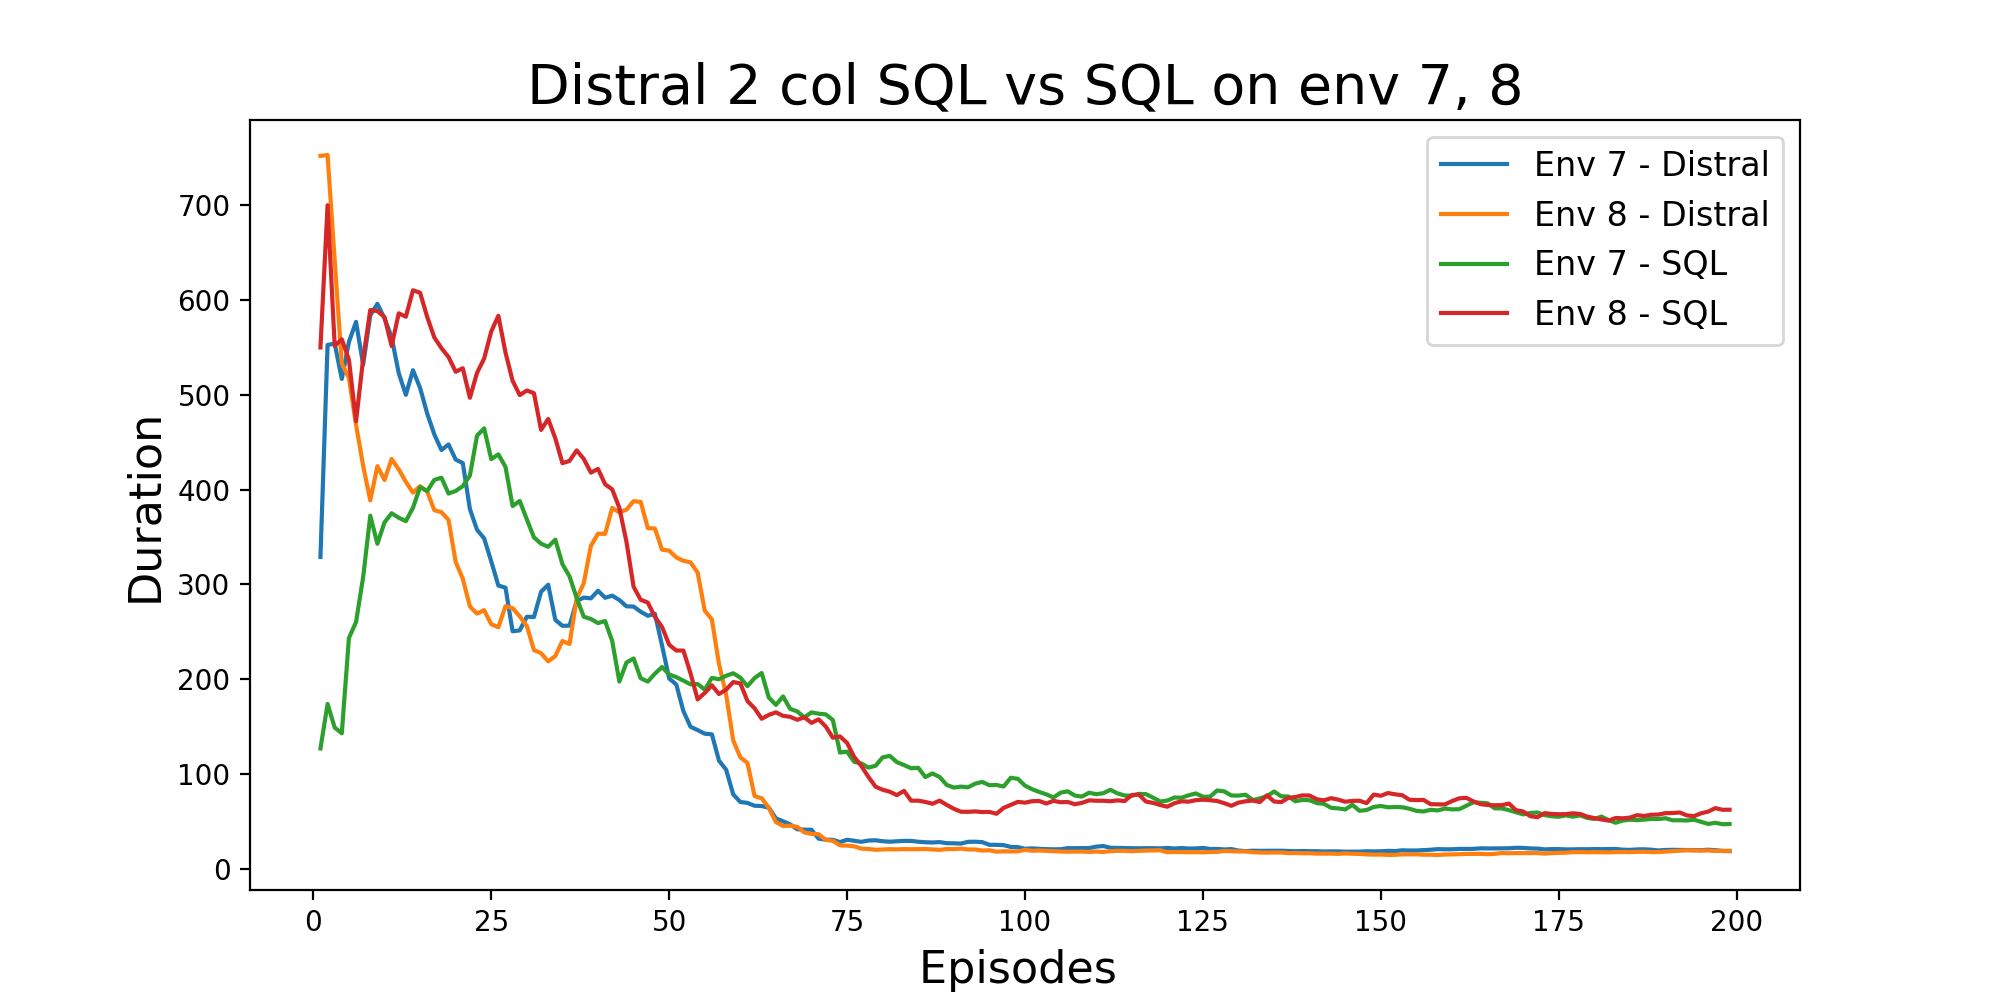
\includegraphics[width=\textwidth]{figs/d2_col_sql/d2_col_sql_7_8_dur.png}
\end{minipage}%
\end{figure}
For environments 7 and 8 we see again that Distral 2 col converges at around episode 50, although performing worse than the SQL baseline initially.

\subsubsection{Environments 4, 5 and 7}
\begin{figure}[H]
\centering
\begin{minipage}{.5\textwidth}
\centering
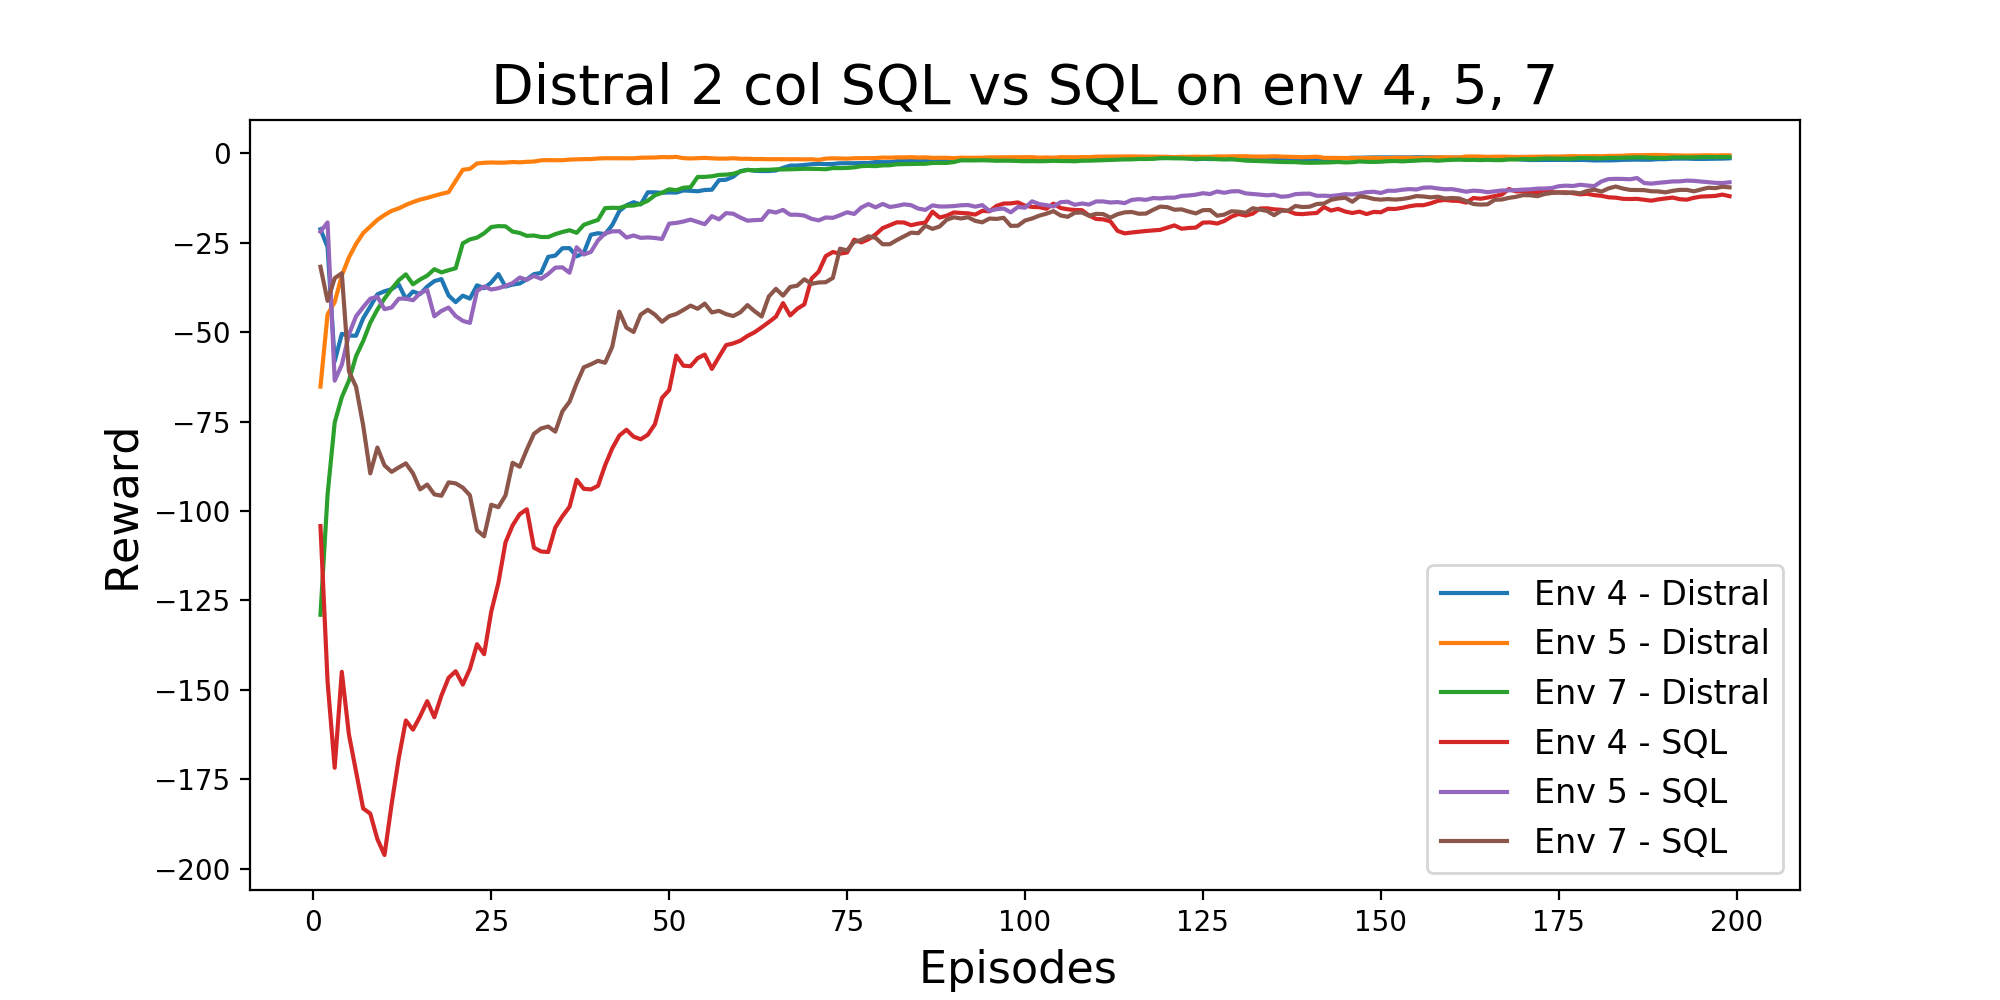
\includegraphics[width=\textwidth]{figs/d2_col_sql/d2_col_sql_4_5_7_rwd.png}
\end{minipage}%
\centering
\begin{minipage}{.5\textwidth}
\centering
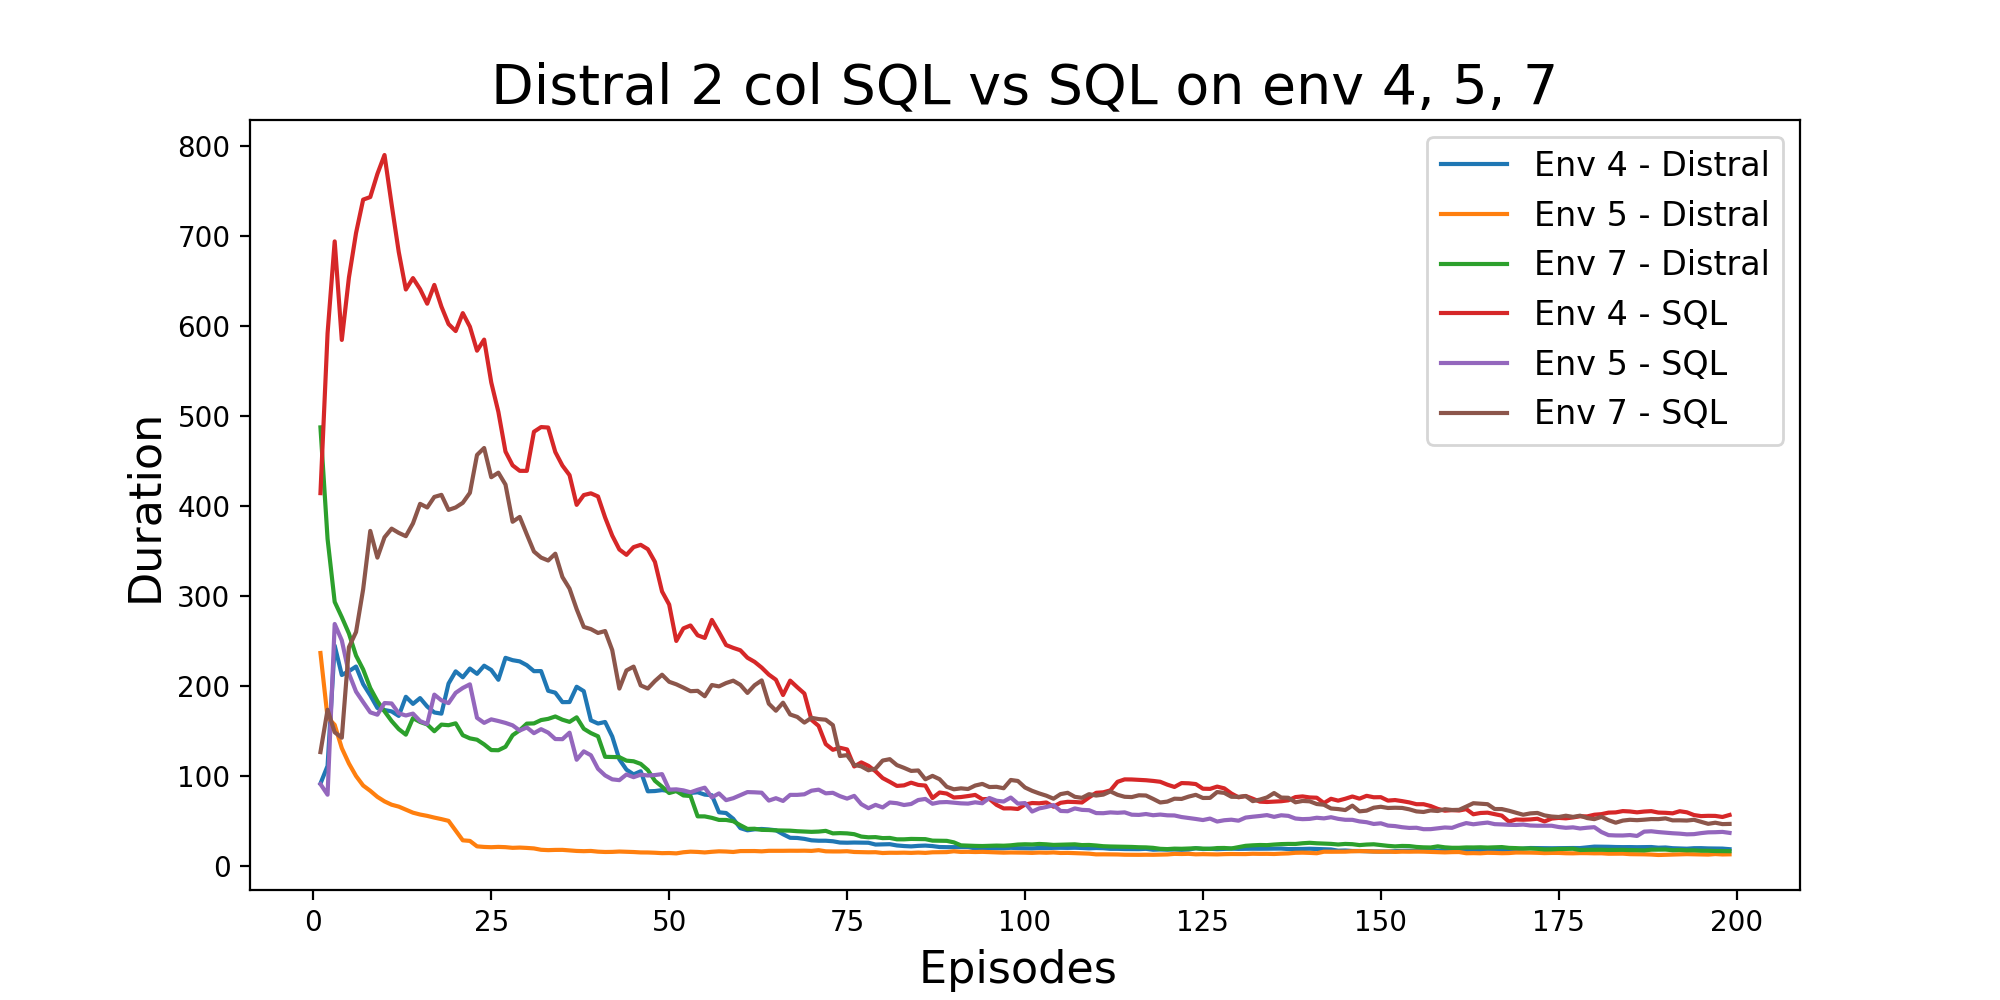
\includegraphics[width=\textwidth]{figs/d2_col_sql/d2_col_sql_4_5_7_dur.png}
\end{minipage}%
\end{figure}
We see that for environments 4, 5 and 7 Distral 2 col converges quicker and performs better than the baseline for the entire 200 episodes.

\subsubsection{Environments 4, 5, 6, 7, 8}
\begin{figure}[H]
\centering
\begin{minipage}{.5\textwidth}
\centering
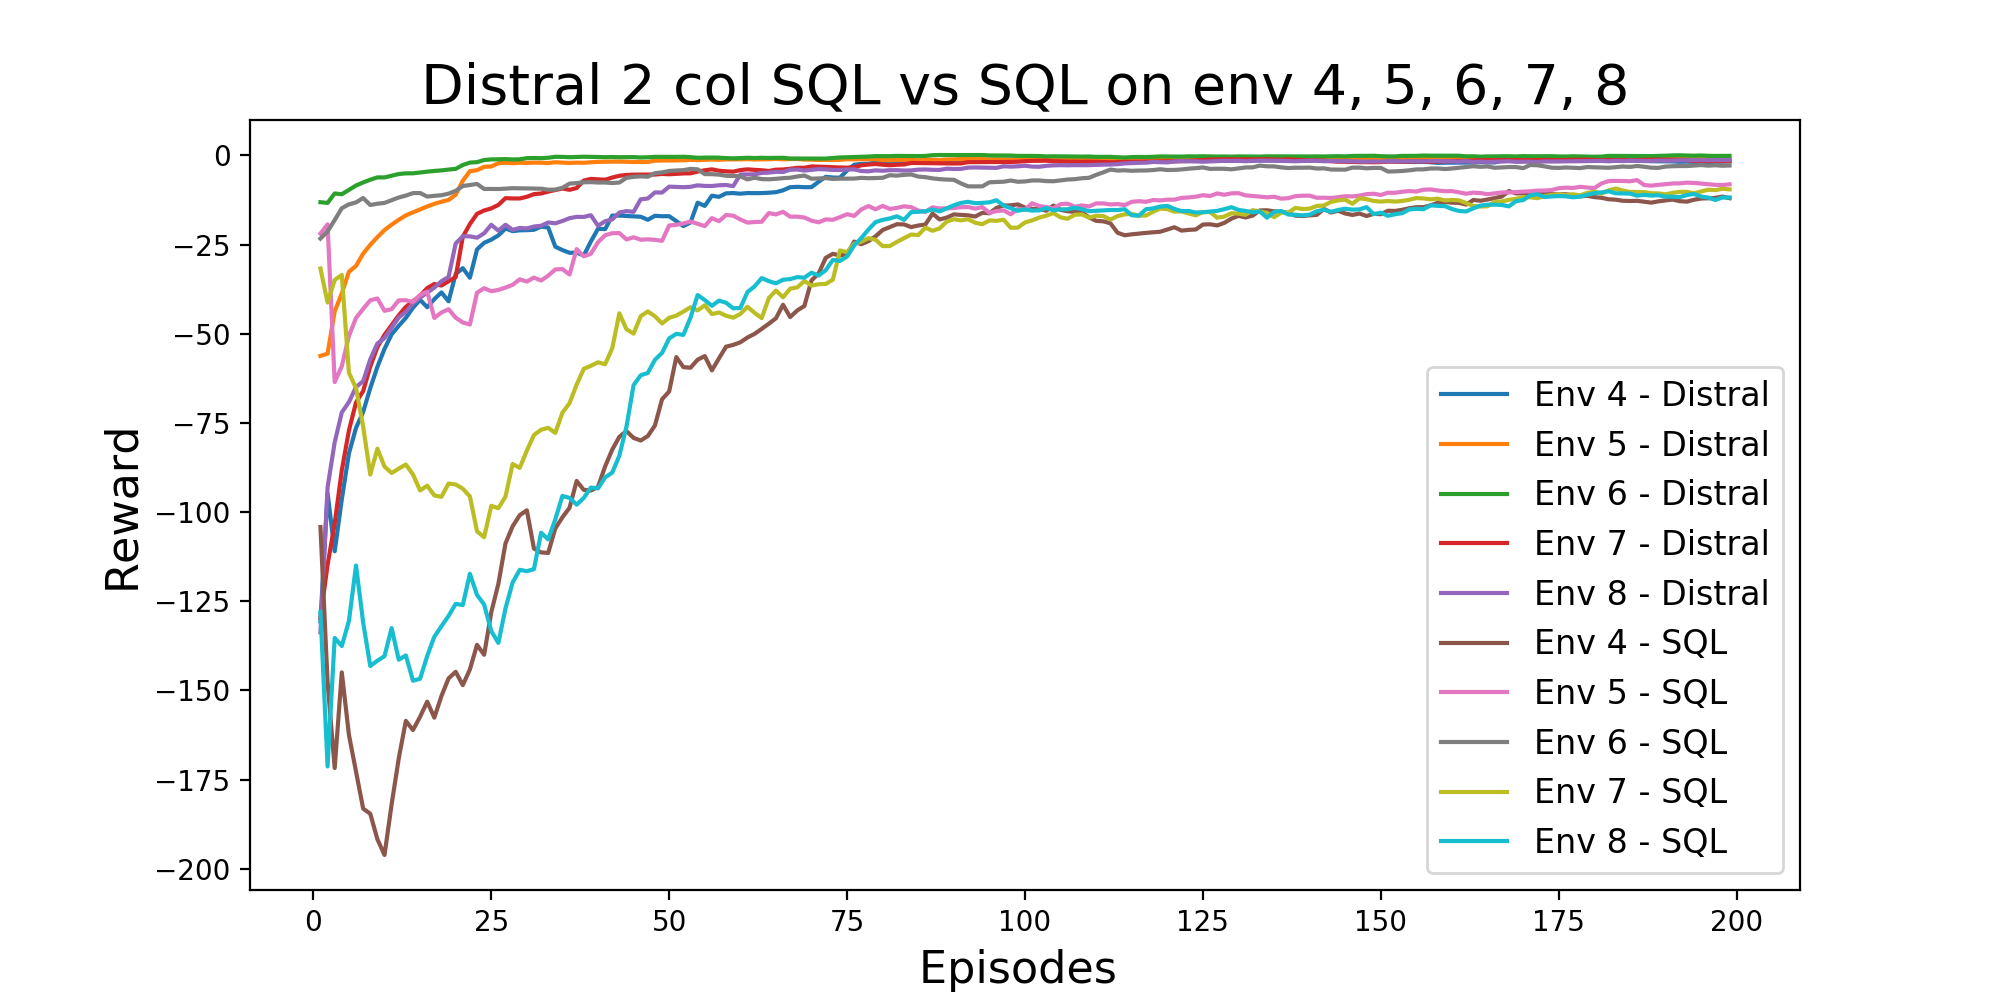
\includegraphics[width=\textwidth]{figs/d2_col_sql/d2_col_sql_4_5_6_7_8_rwd.png}
\end{minipage}%
\centering
\begin{minipage}{.5\textwidth}
\centering
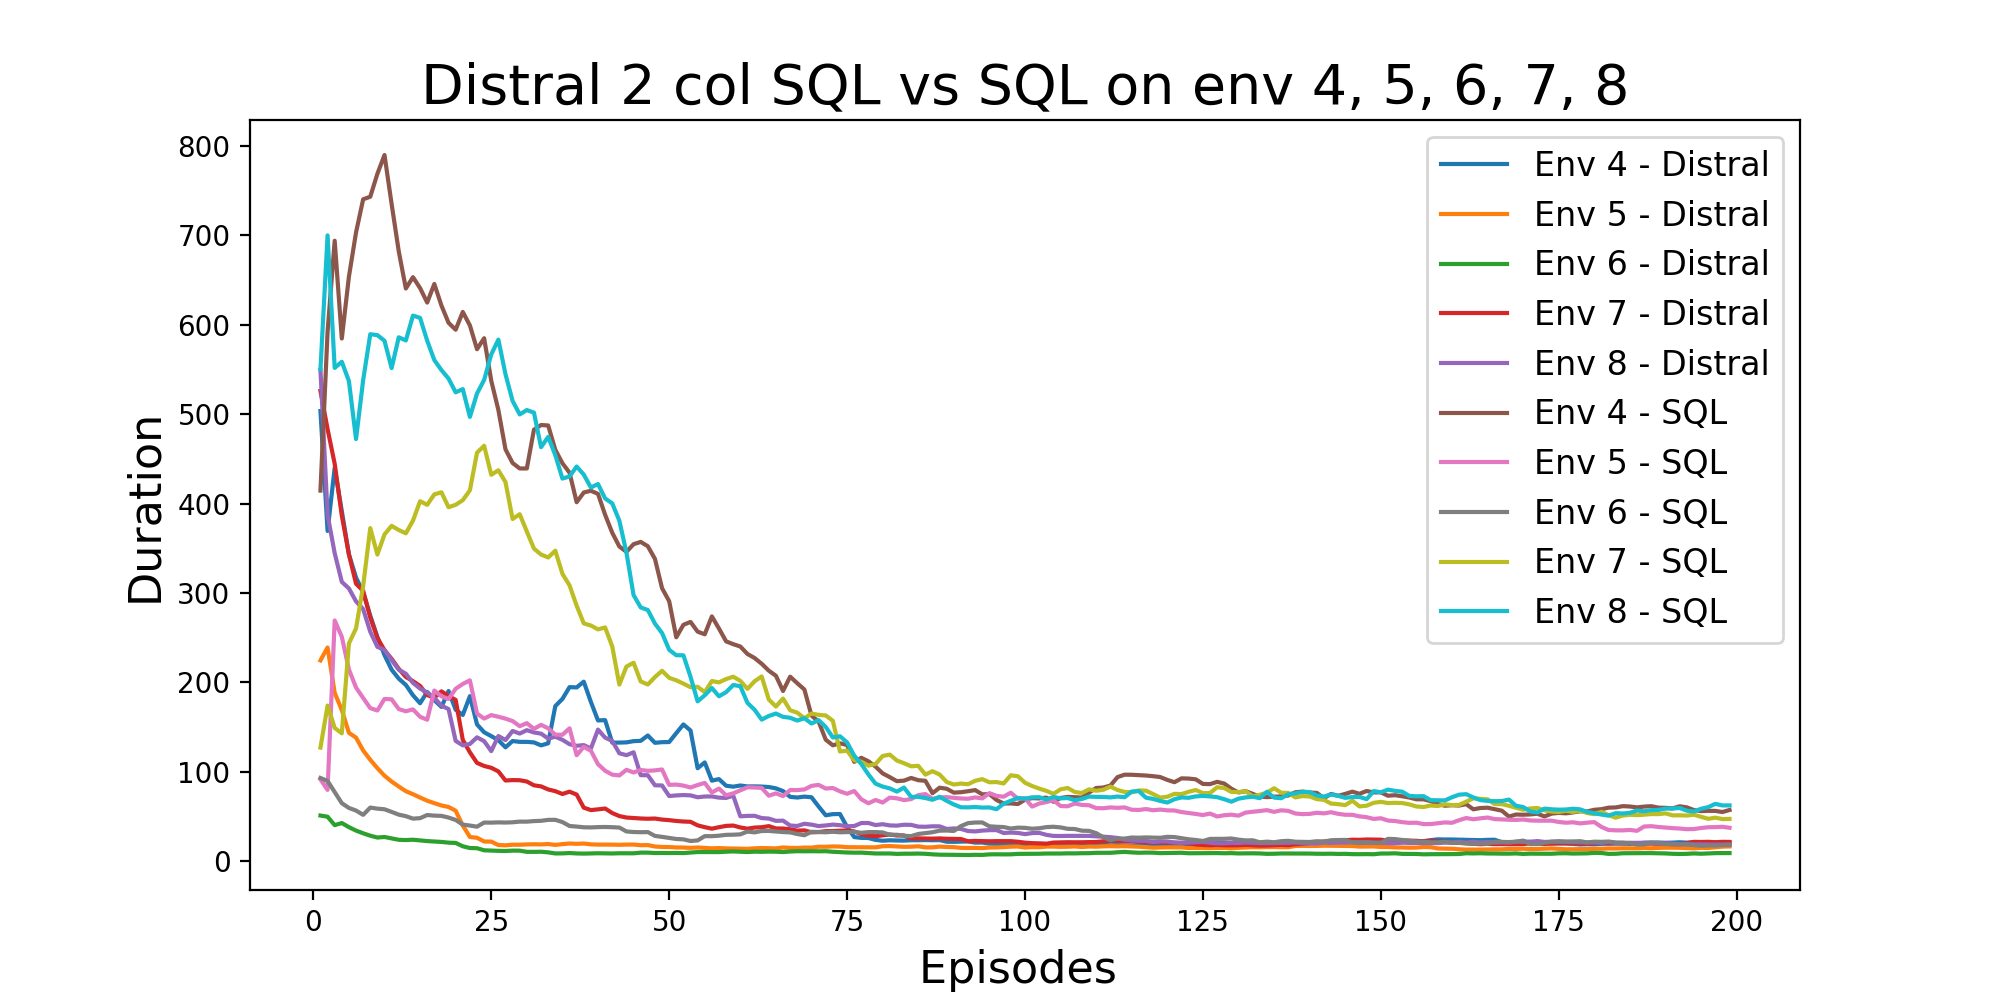
\includegraphics[width=\textwidth]{figs/d2_col_sql/d2_col_sql_4_5_6_7_8_dur.png}
\end{minipage}%
\end{figure}
We also see that the algorithm performs worse when it is dealing with more environments. This can be further demonstrated in the following results, where Distral 2 col is trained simultaneously on environments 4, 5, 6, 7, and 8.

\section{Experiments under regularized AC framework}

In this section we will compare the performance of Distral 1 col and Distral 2 col versus A3C in same maze environments as the previous experiments with SQL. Both Distral algorithms will be implemented under the regularized AC framework as demonstrated in the pseudocode for algorithm \ref{alg:dist1colAC}.

\subsection{Distral 1 col vs A3C}
\subsubsection{Environment 4 and 5}
\begin{figure}[H]
\centering
\begin{minipage}{.5\textwidth}
\centering
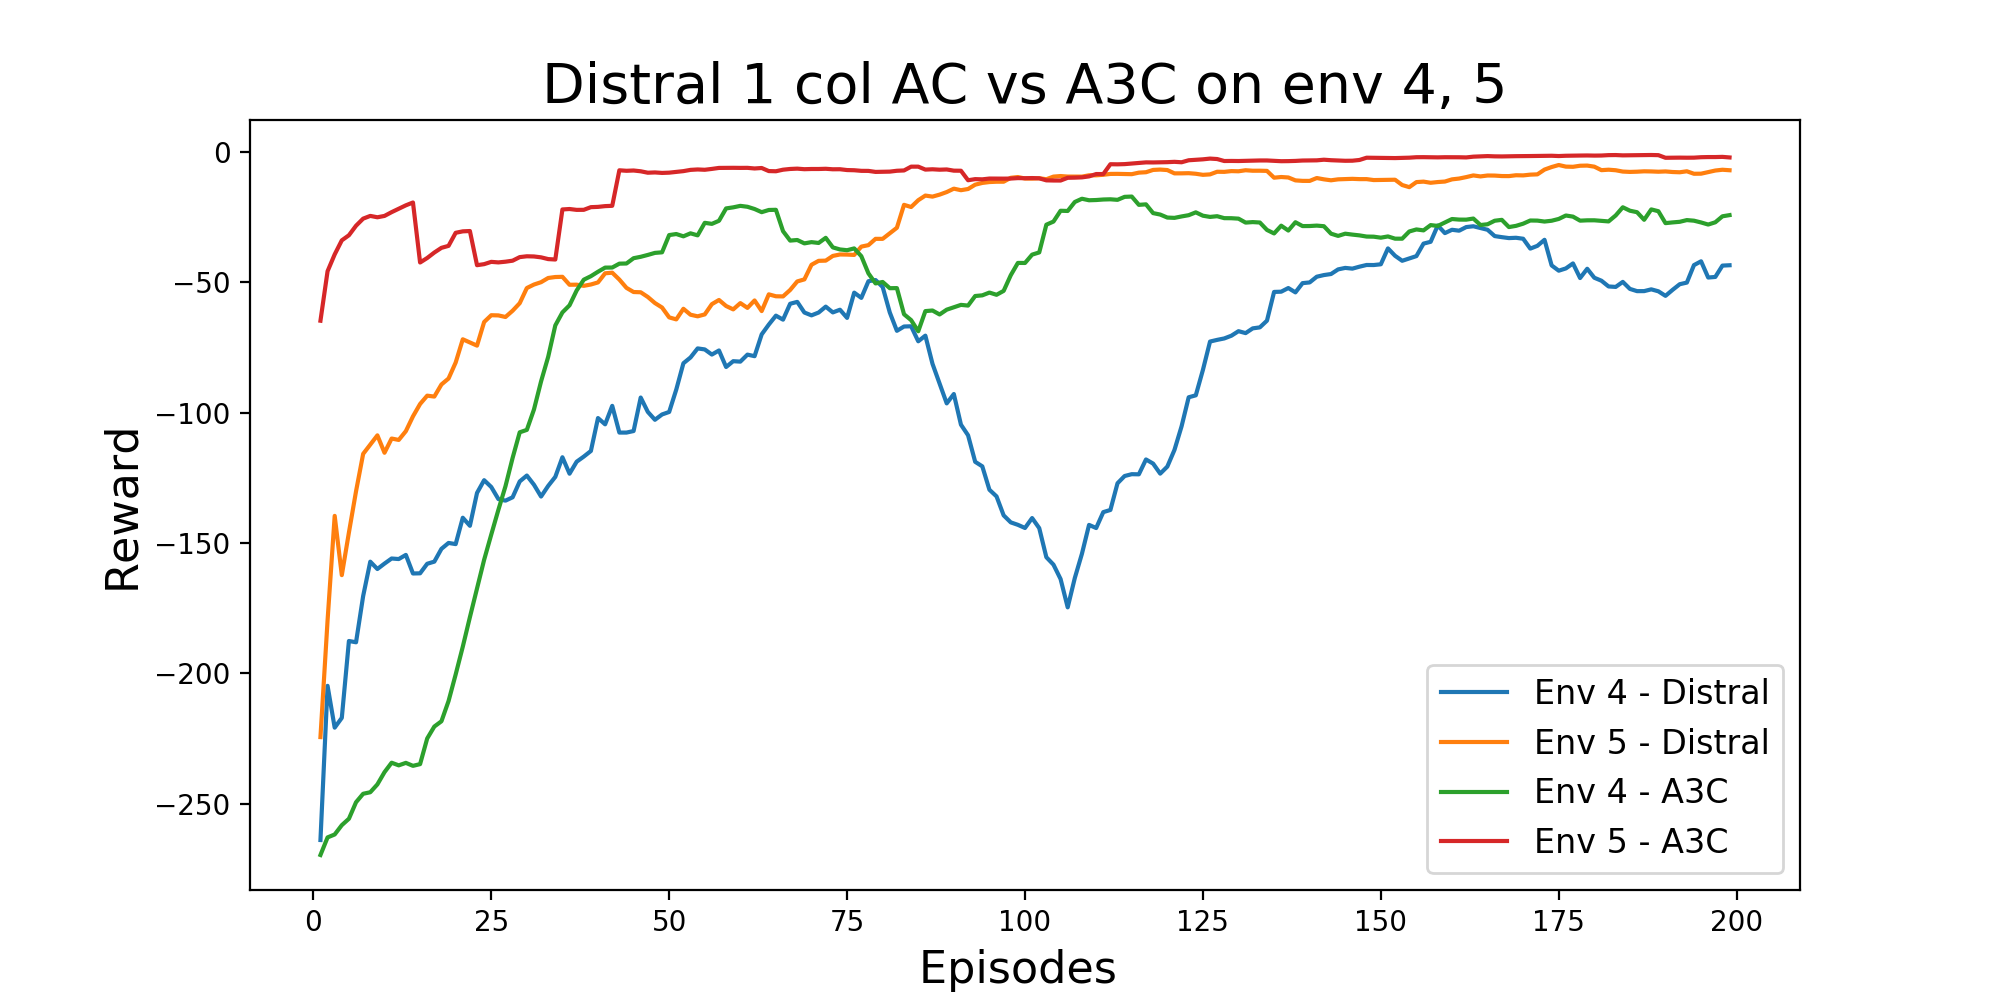
\includegraphics[width=\textwidth]{figs/d1_col_ac/d1_col_ac_4_5_rwd.png}
\end{minipage}%
\centering
\begin{minipage}{.5\textwidth}
\centering
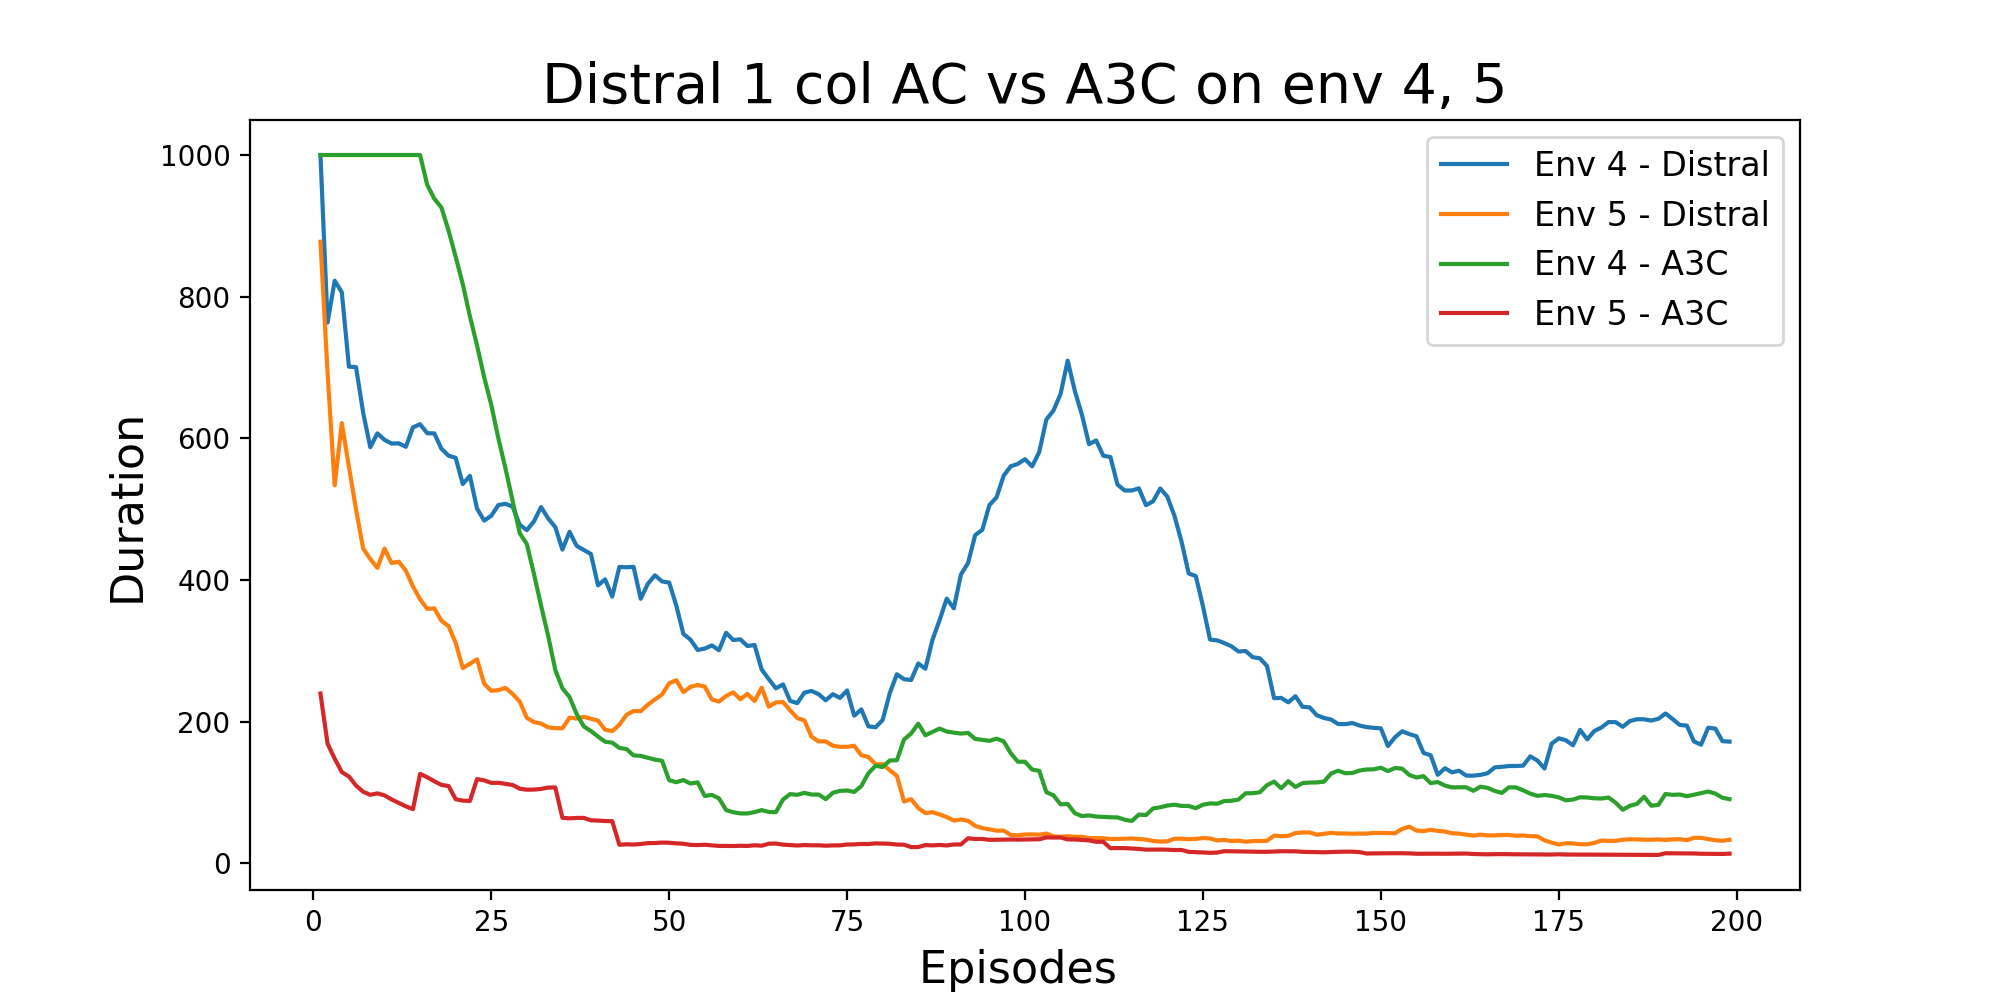
\includegraphics[width=\textwidth]{figs/d1_col_ac/d1_col_ac_4_5_dur.png}
\end{minipage}%
\end{figure}
As shown above, Distral 1 col via regularized Actor Critic exhibits the similar behaviour to Distral 1 col implemented using SQL. For both algorithms, the duration for environment 4 plateaus around 200 steps. 

\subsubsection{Environment 7 and 8}
\begin{figure}[H]
\centering
\begin{minipage}{.5\textwidth}
\centering
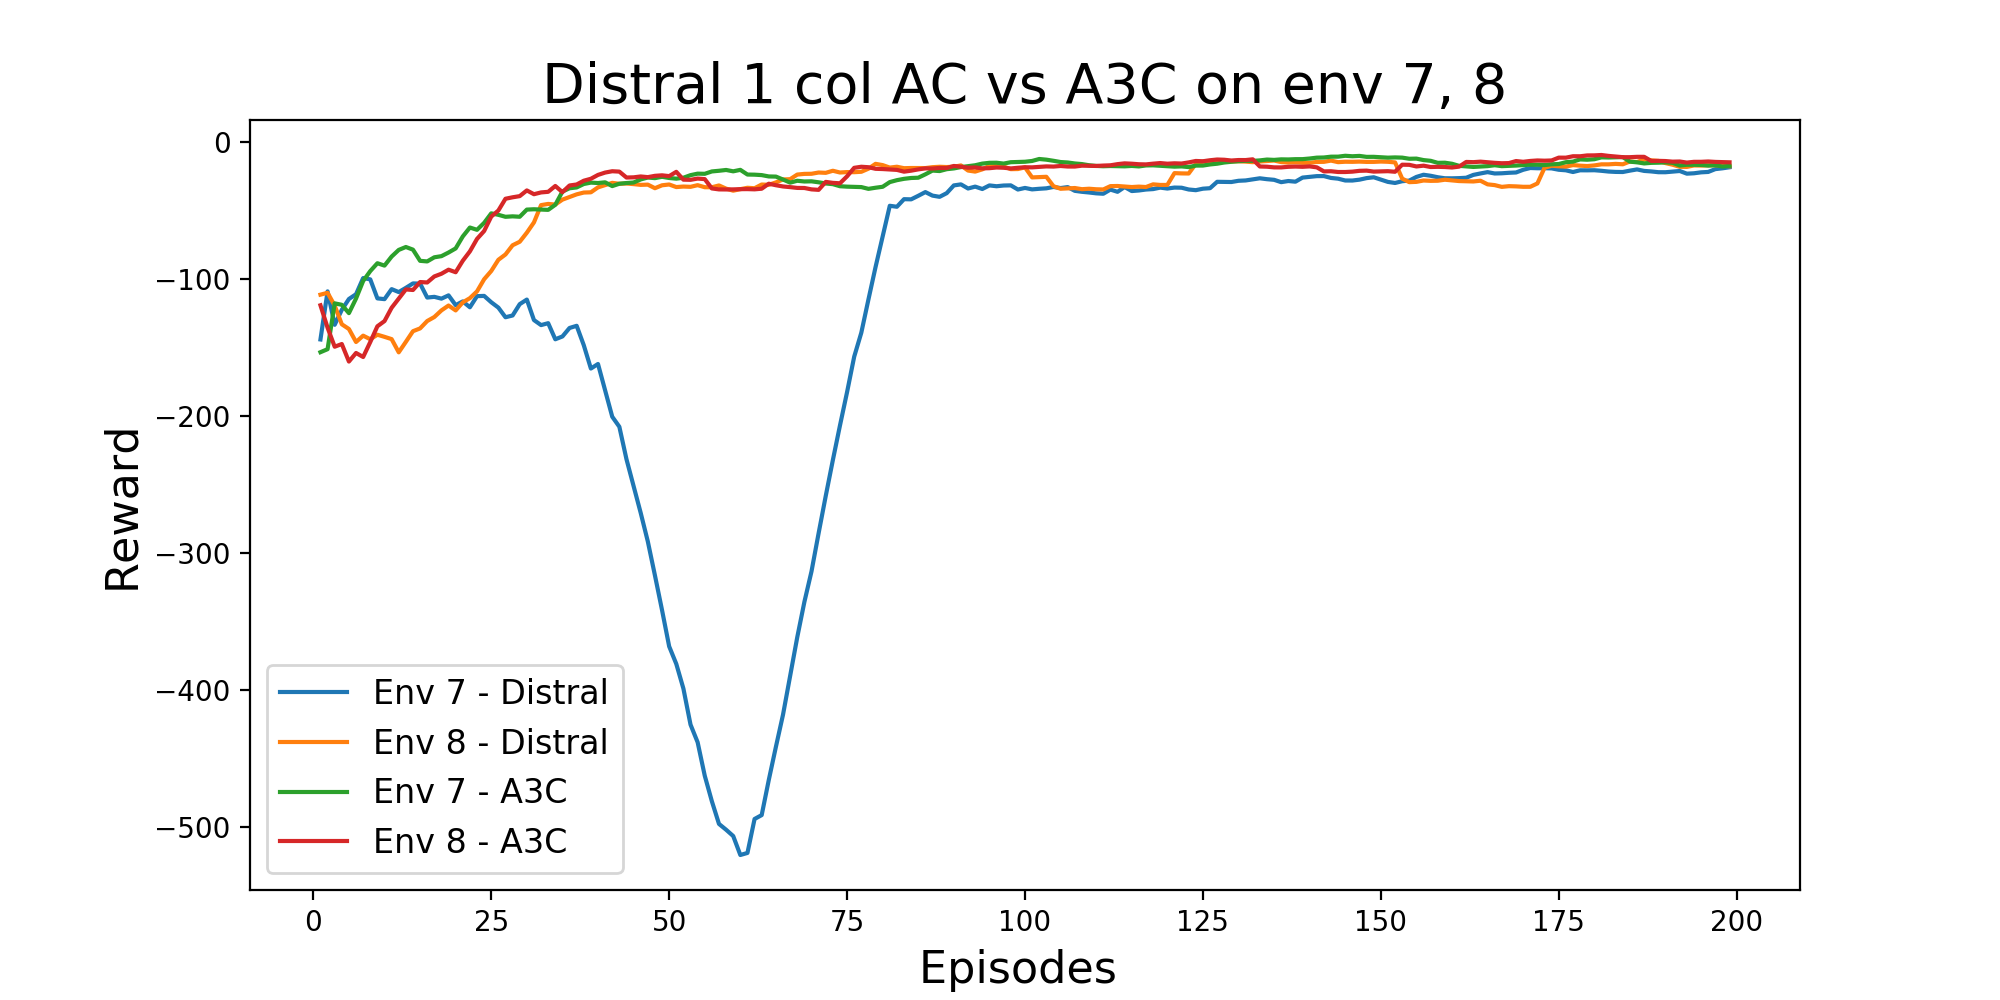
\includegraphics[width=\textwidth]{figs/d1_col_ac/d1_col_ac_7_8_rwd.png}
\end{minipage}%
\centering
\begin{minipage}{.5\textwidth}
\centering
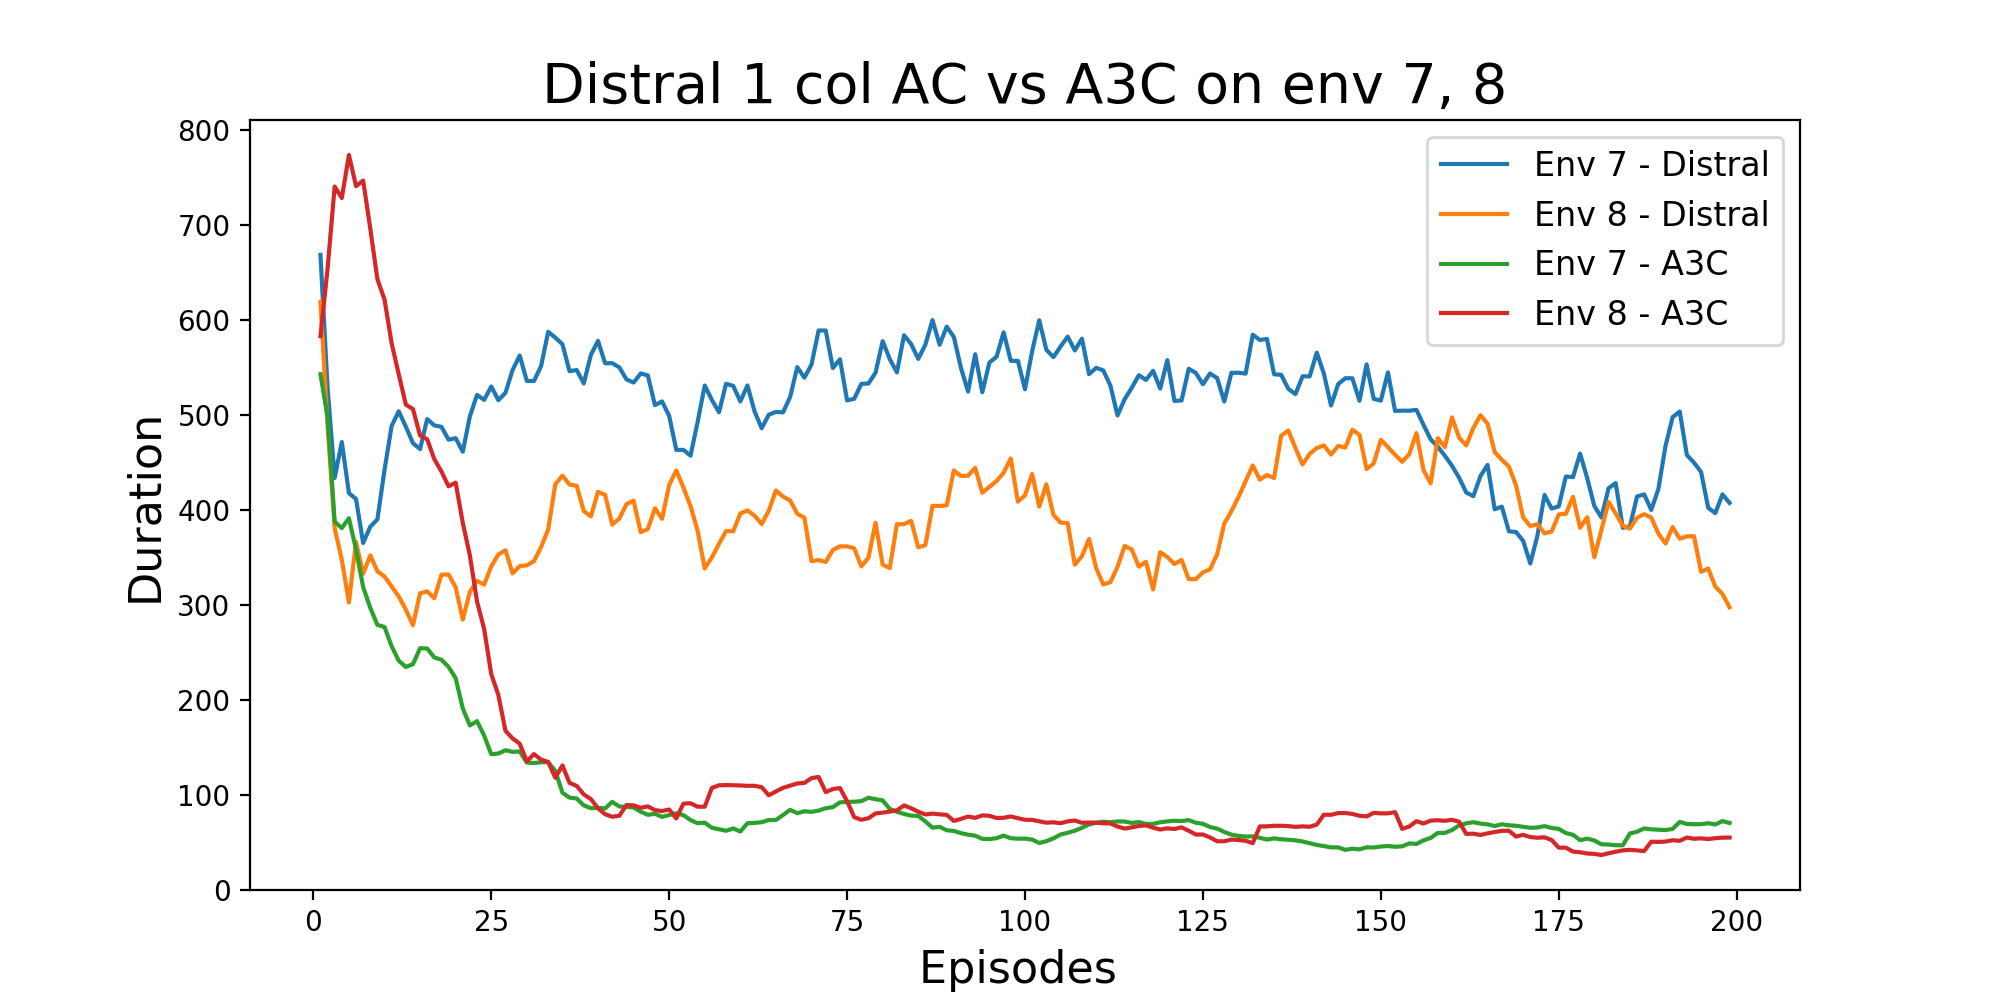
\includegraphics[width=\textwidth]{figs/d1_col_ac/d1_col_ac_7_8_dur.png}
\end{minipage}%
\end{figure}

\subsubsection{Environments 4, 5 and 7}
\begin{figure}[H]
\centering
\begin{minipage}{.5\textwidth}
\centering
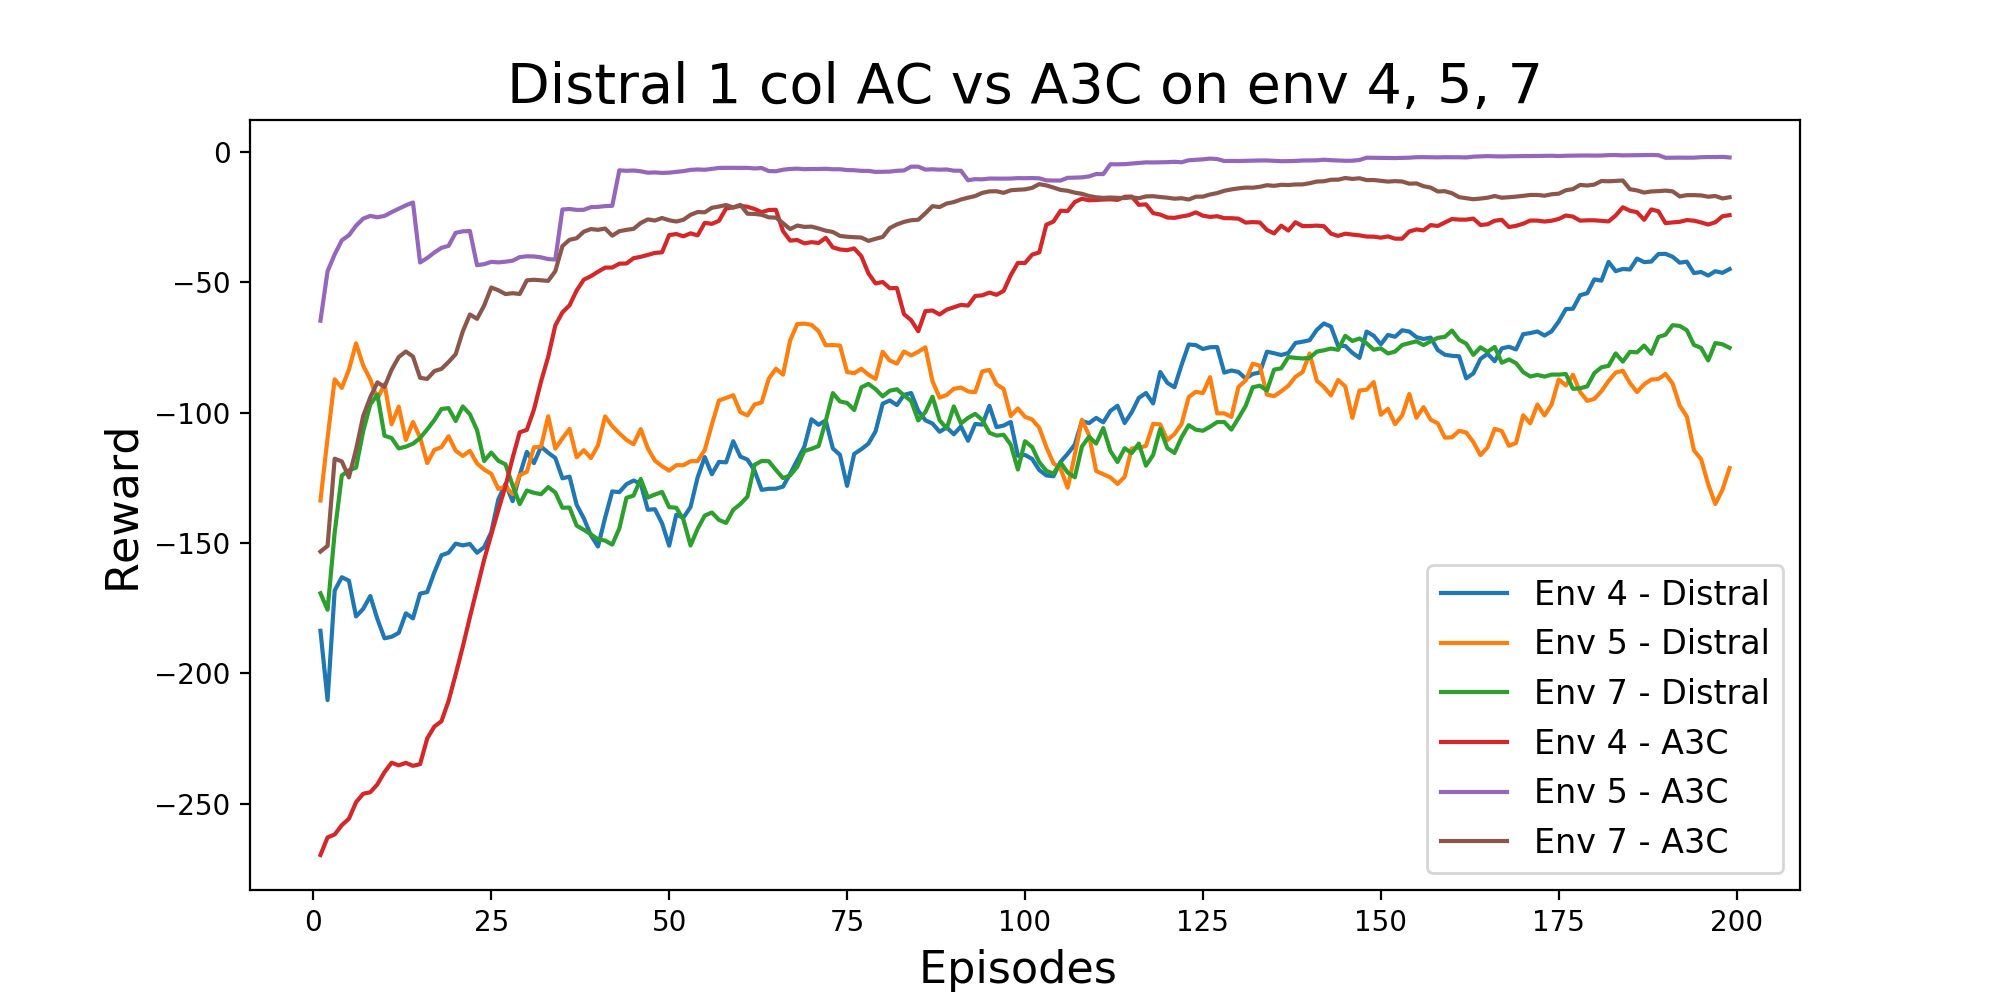
\includegraphics[width=\textwidth]{figs/d1_col_ac/d1_col_ac_4_5_7_rwd.png}
\end{minipage}%
\centering
\begin{minipage}{.5\textwidth}
\centering
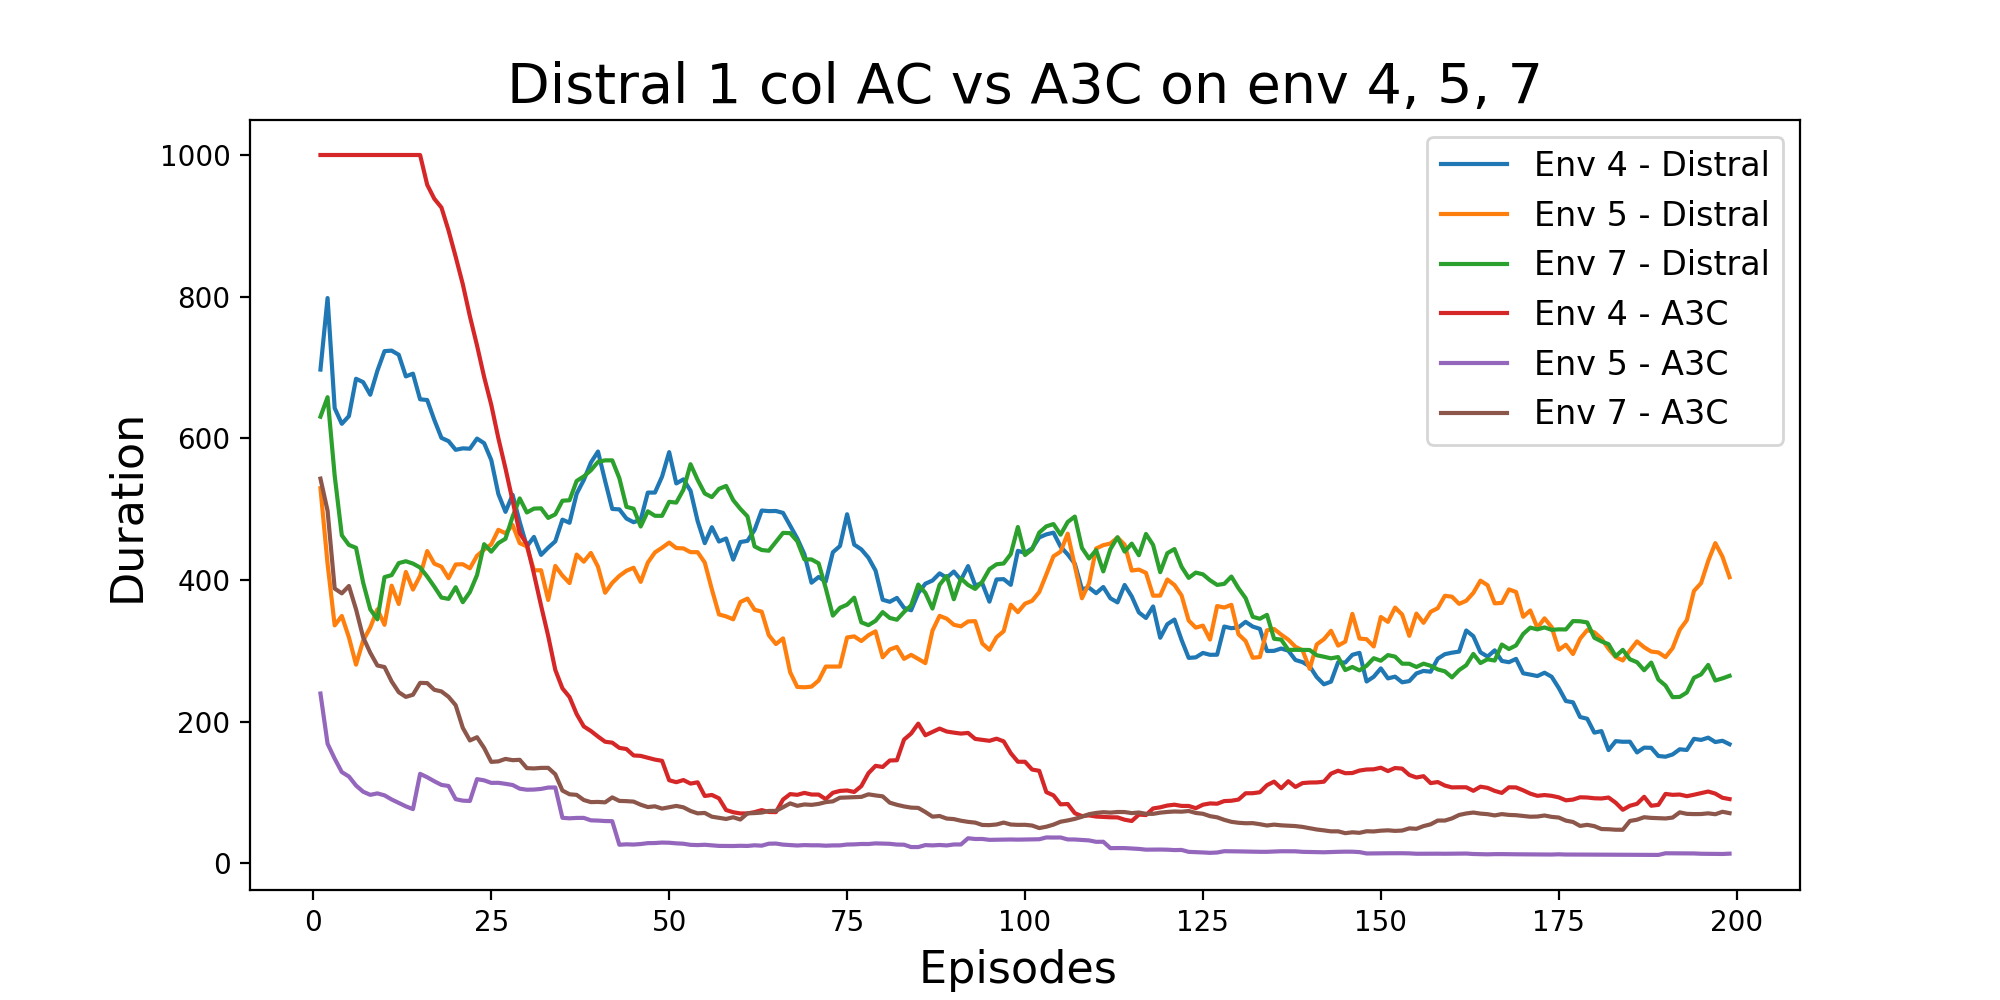
\includegraphics[width=\textwidth]{figs/d1_col_ac/d1_col_ac_4_5_7_dur.png}
\end{minipage}%
\end{figure}
Here we observe that the Distral algorithm performs worse as it takes on more environments. Specifically, we see that it did not even manage to find the solution for enviroment 5, which is an easy environment compared to 5 and 7.

\subsubsection{Environments 4, 5, 6, 7, 8}
\begin{figure}[H]
\centering
\begin{minipage}{.5\textwidth}
\centering
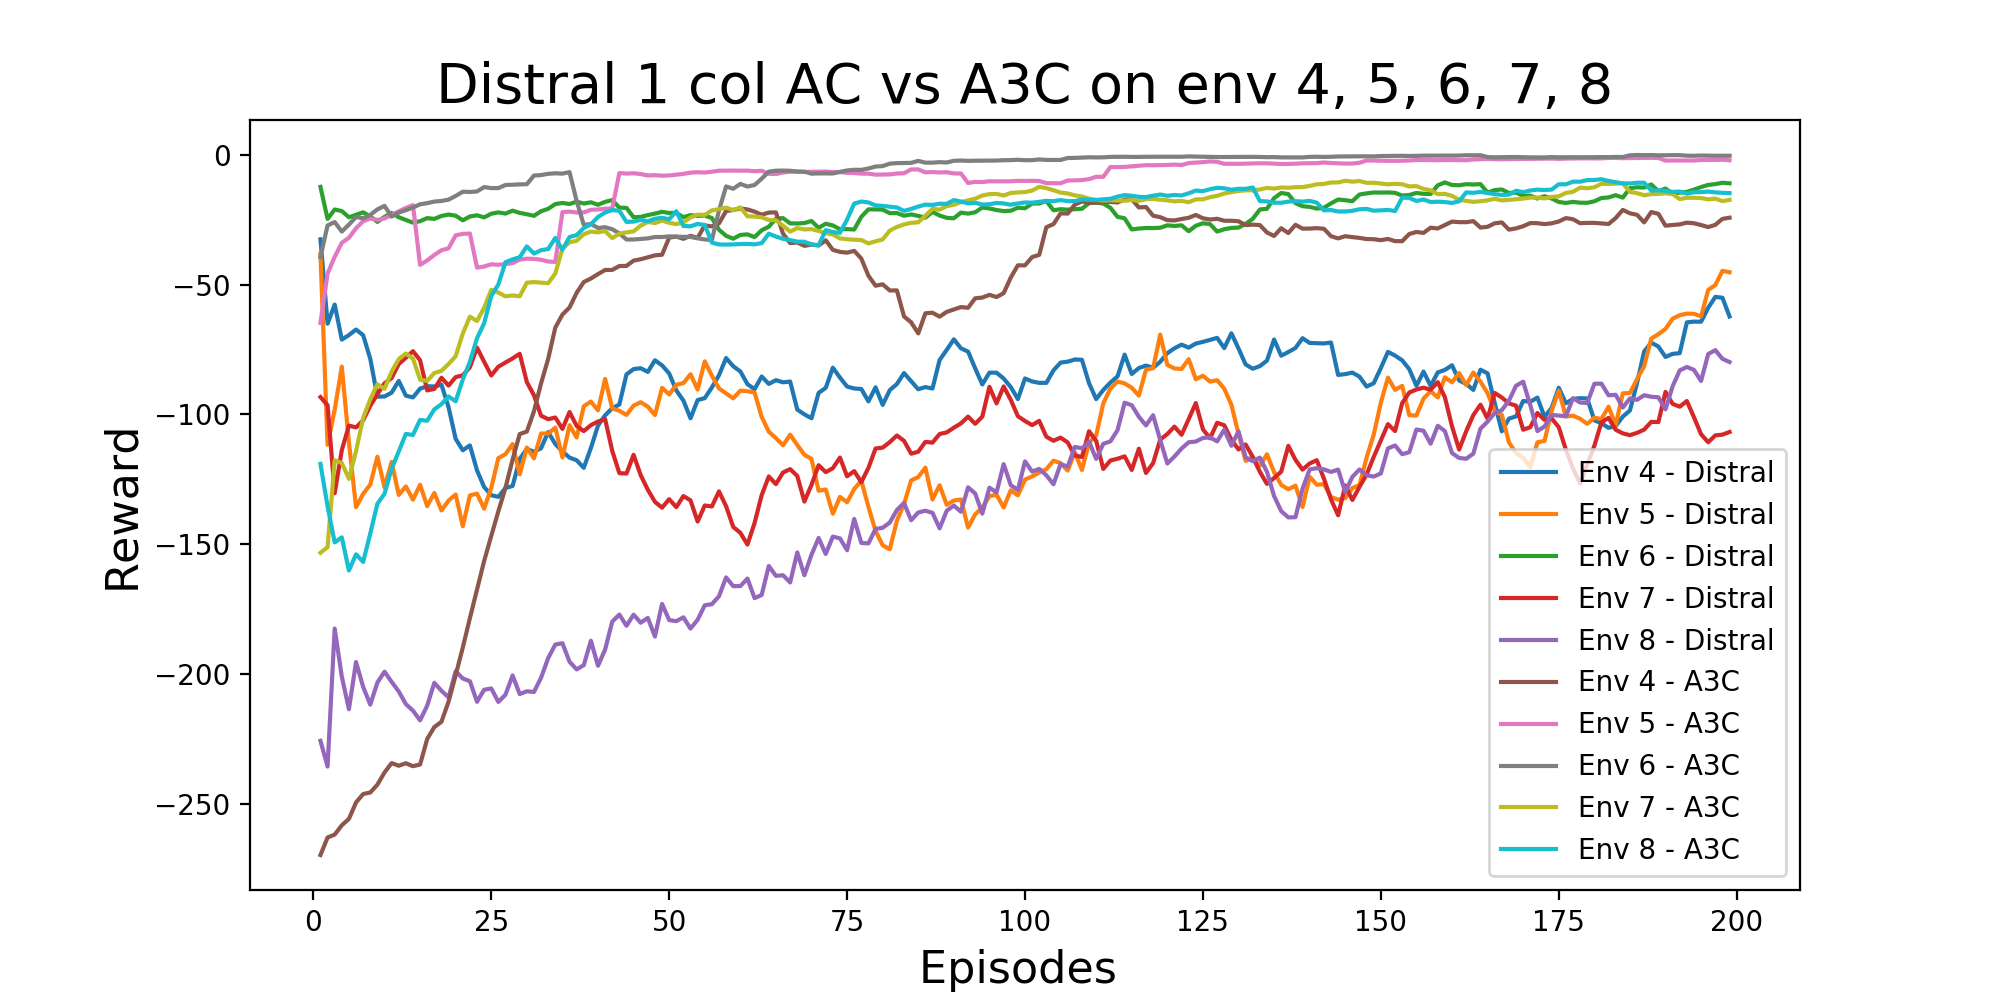
\includegraphics[width=\textwidth]{figs/d1_col_ac/d1_col_ac_4_5_6_7_8_rwd.png}
\end{minipage}%
\centering
\begin{minipage}{.5\textwidth}
\centering
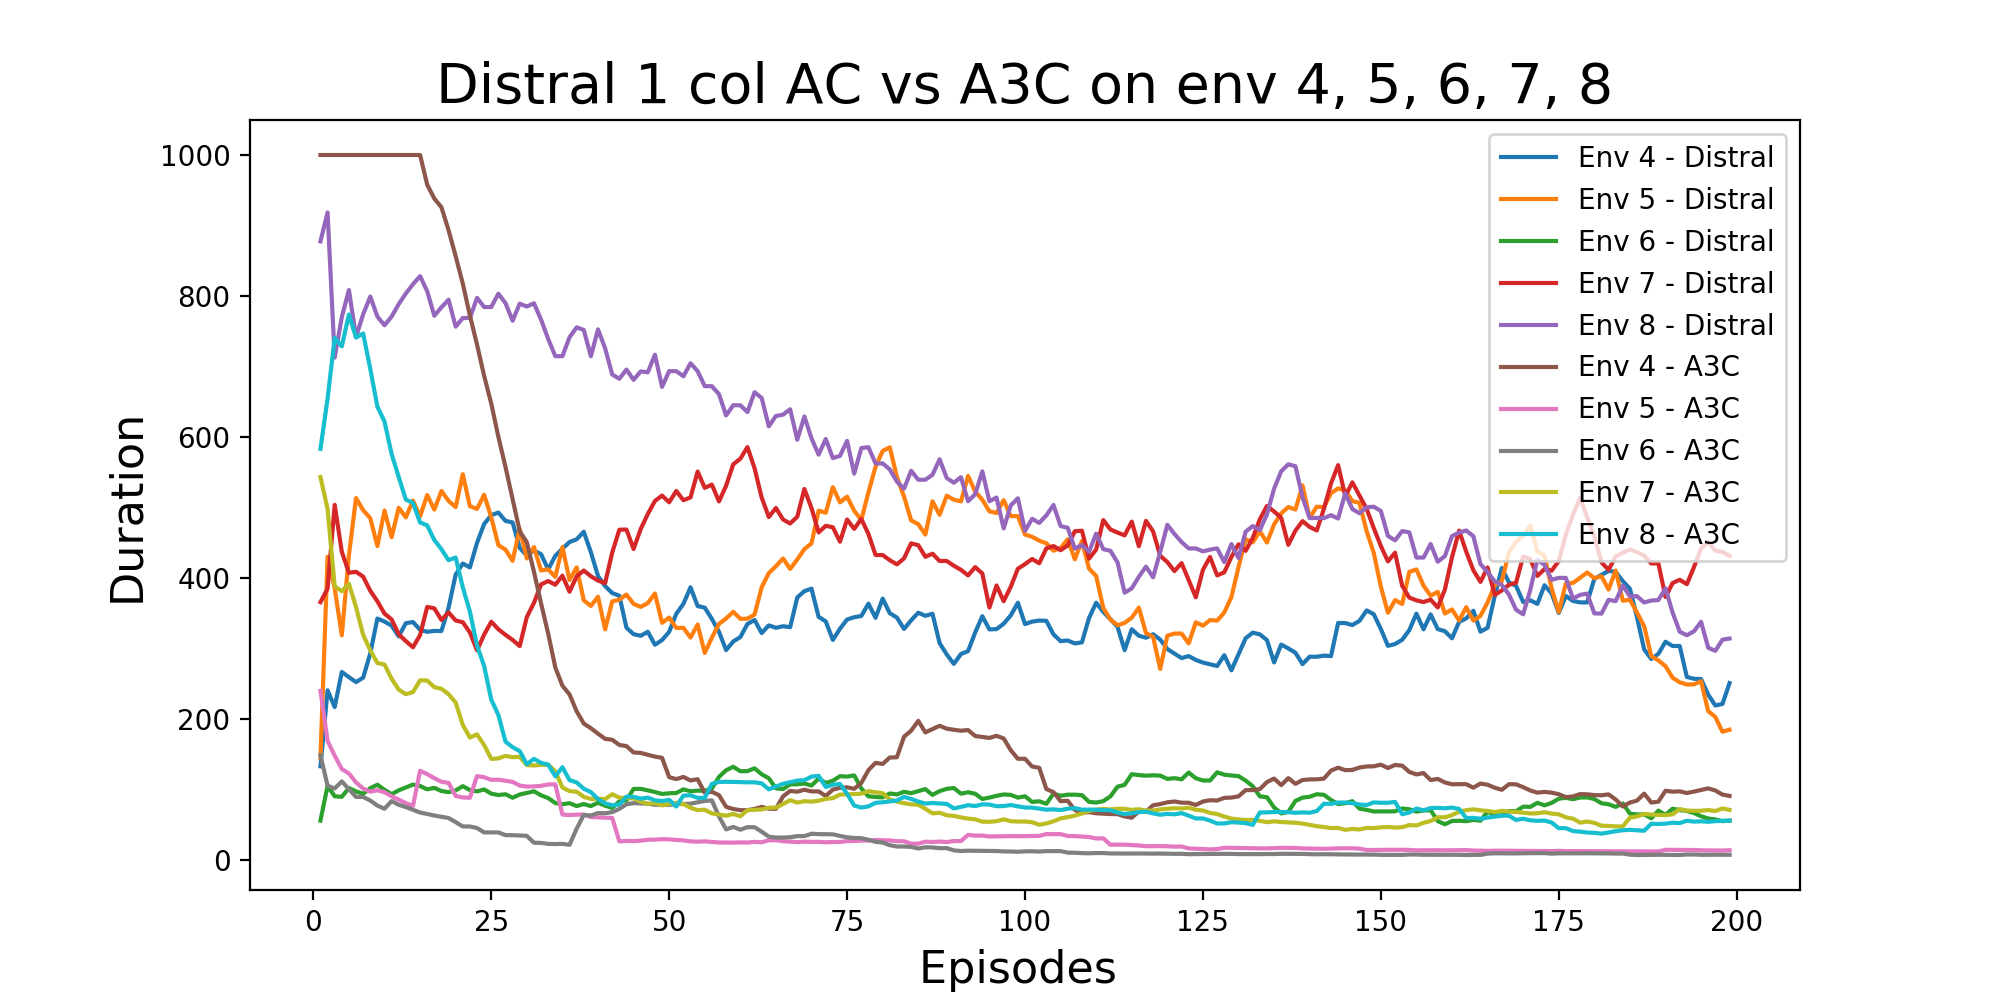
\includegraphics[width=\textwidth]{figs/d1_col_ac/d1_col_ac_4_5_6_7_8_dur.png}
\end{minipage}%
\end{figure}
Here we see that the behaviour of the algorithm is consistent with previous observations. None of the environments were solved.

\subsection{Distral 2 col vs A3C}
\subsubsection{Environment 4 and 5}
\begin{figure}[H]
\centering
\begin{minipage}{.5\textwidth}
\centering
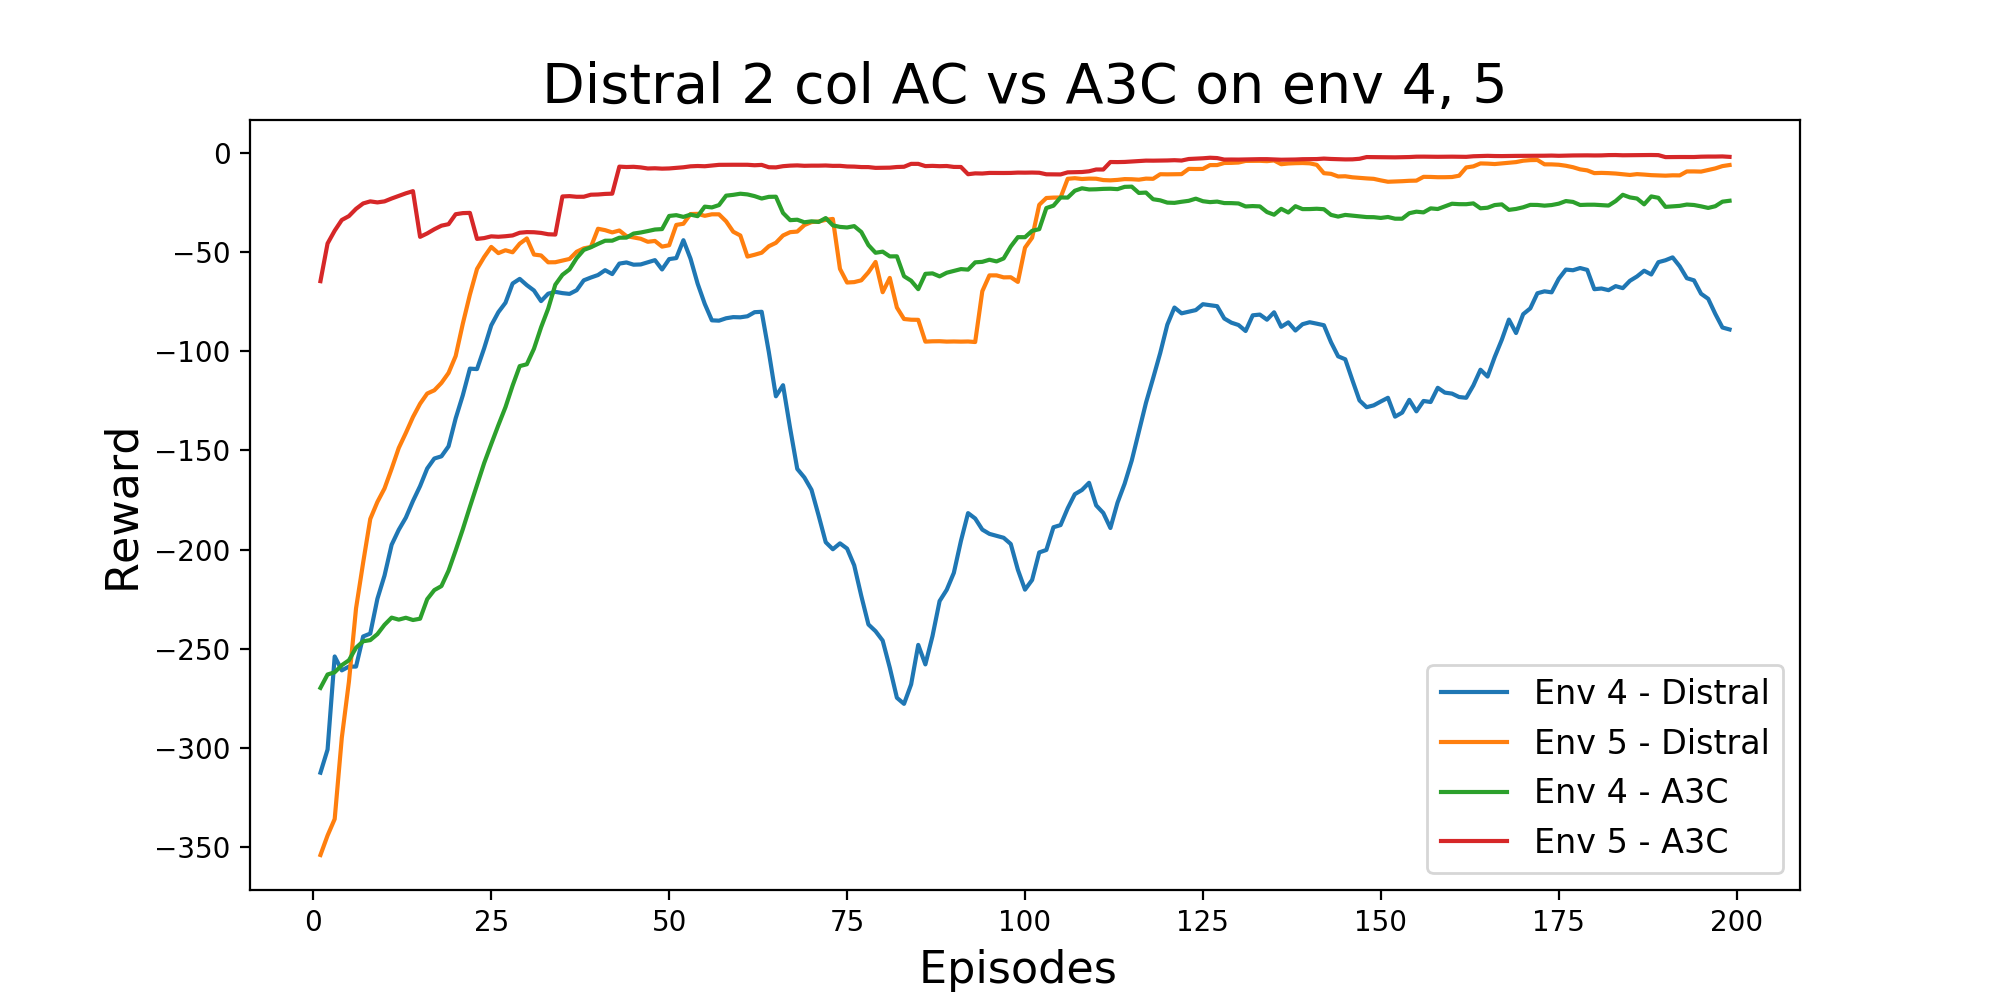
\includegraphics[width=\textwidth]{figs/d2_col_ac/d2_col_ac_4_5_rwd.png}
\end{minipage}%
\centering
\begin{minipage}{.5\textwidth}
\centering
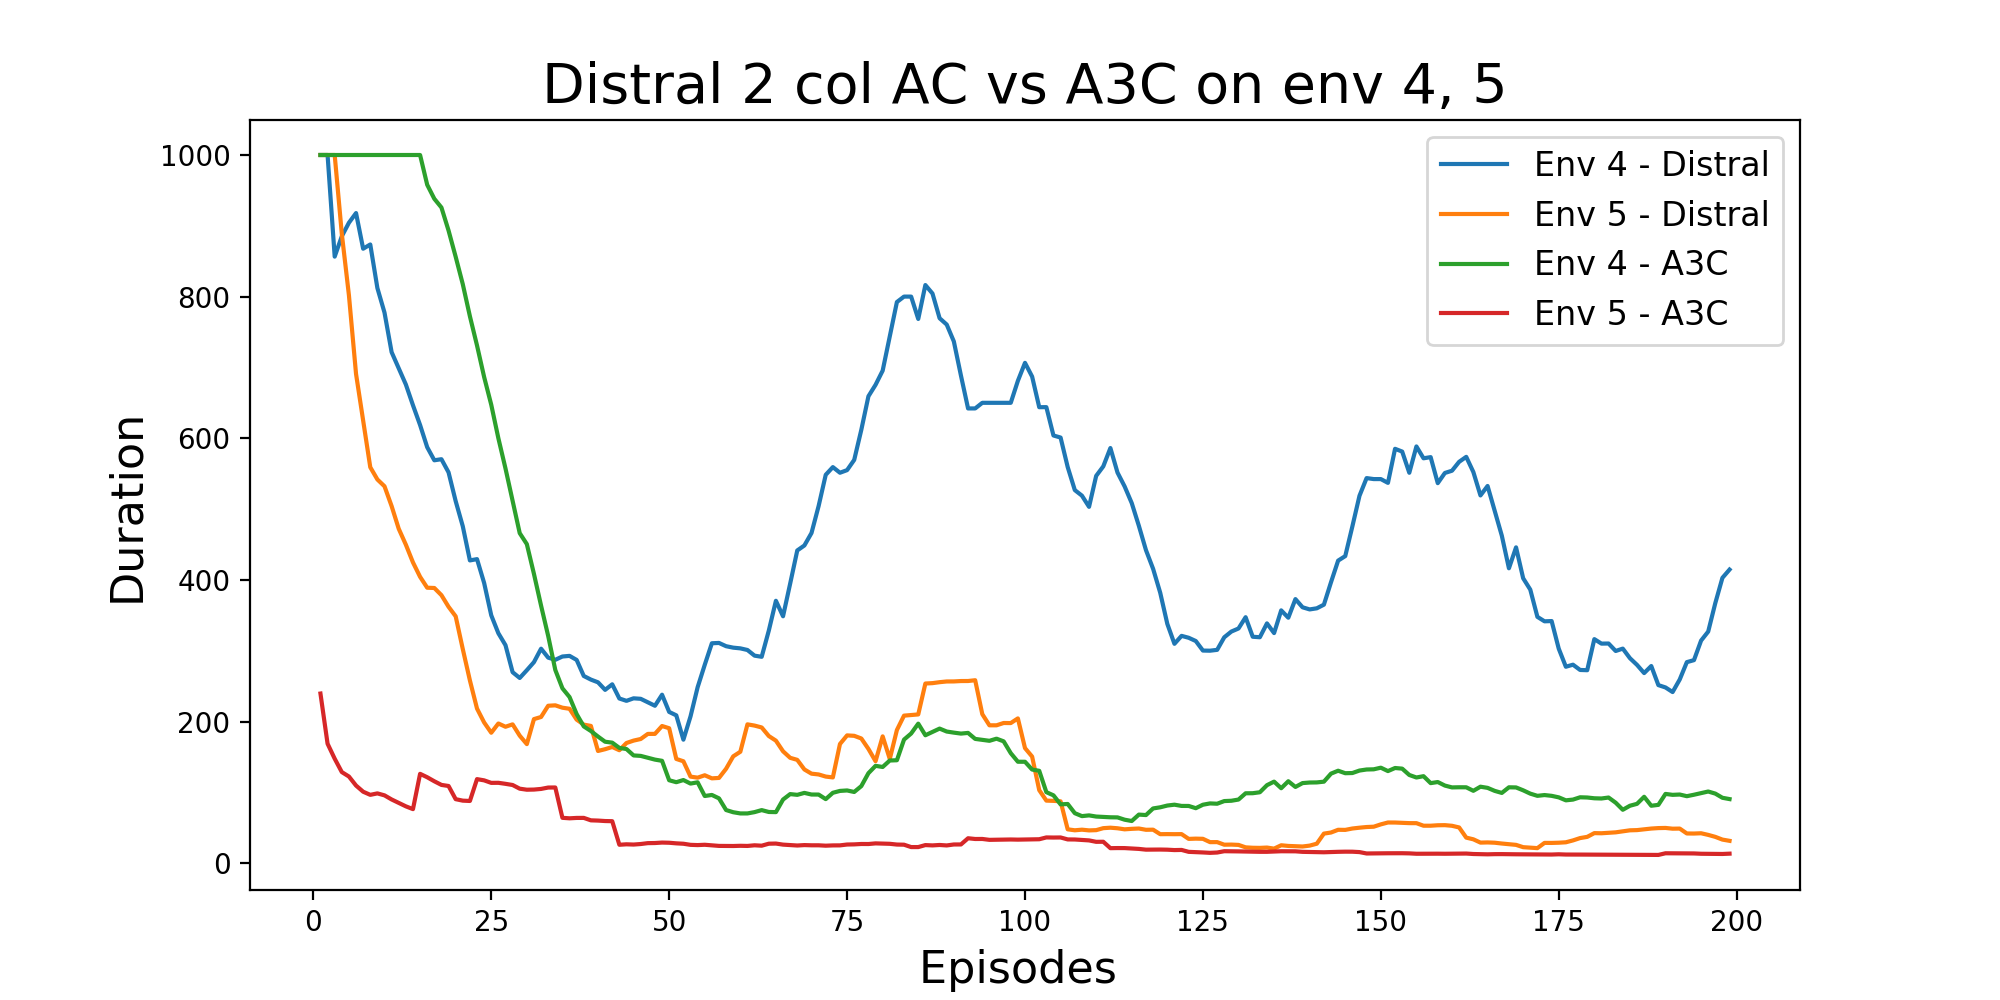
\includegraphics[width=\textwidth]{figs/d2_col_ac/d2_col_ac_4_5_dur.png}
\end{minipage}%
\end{figure}
Here we see that Distral 2 col under AC framework exhibits similar behaviour compared to Distral 1 col under Ac. Specifically, we see that environment 4 did not converge and has consistently taken over 200 episodes to reach the terminal state. However, we should also note that Distral 2 col under AC managed to solve environment 5.

\subsubsection{Environment 7 and 8}
\begin{figure}[H]
\centering
\begin{minipage}{.5\textwidth}
\centering
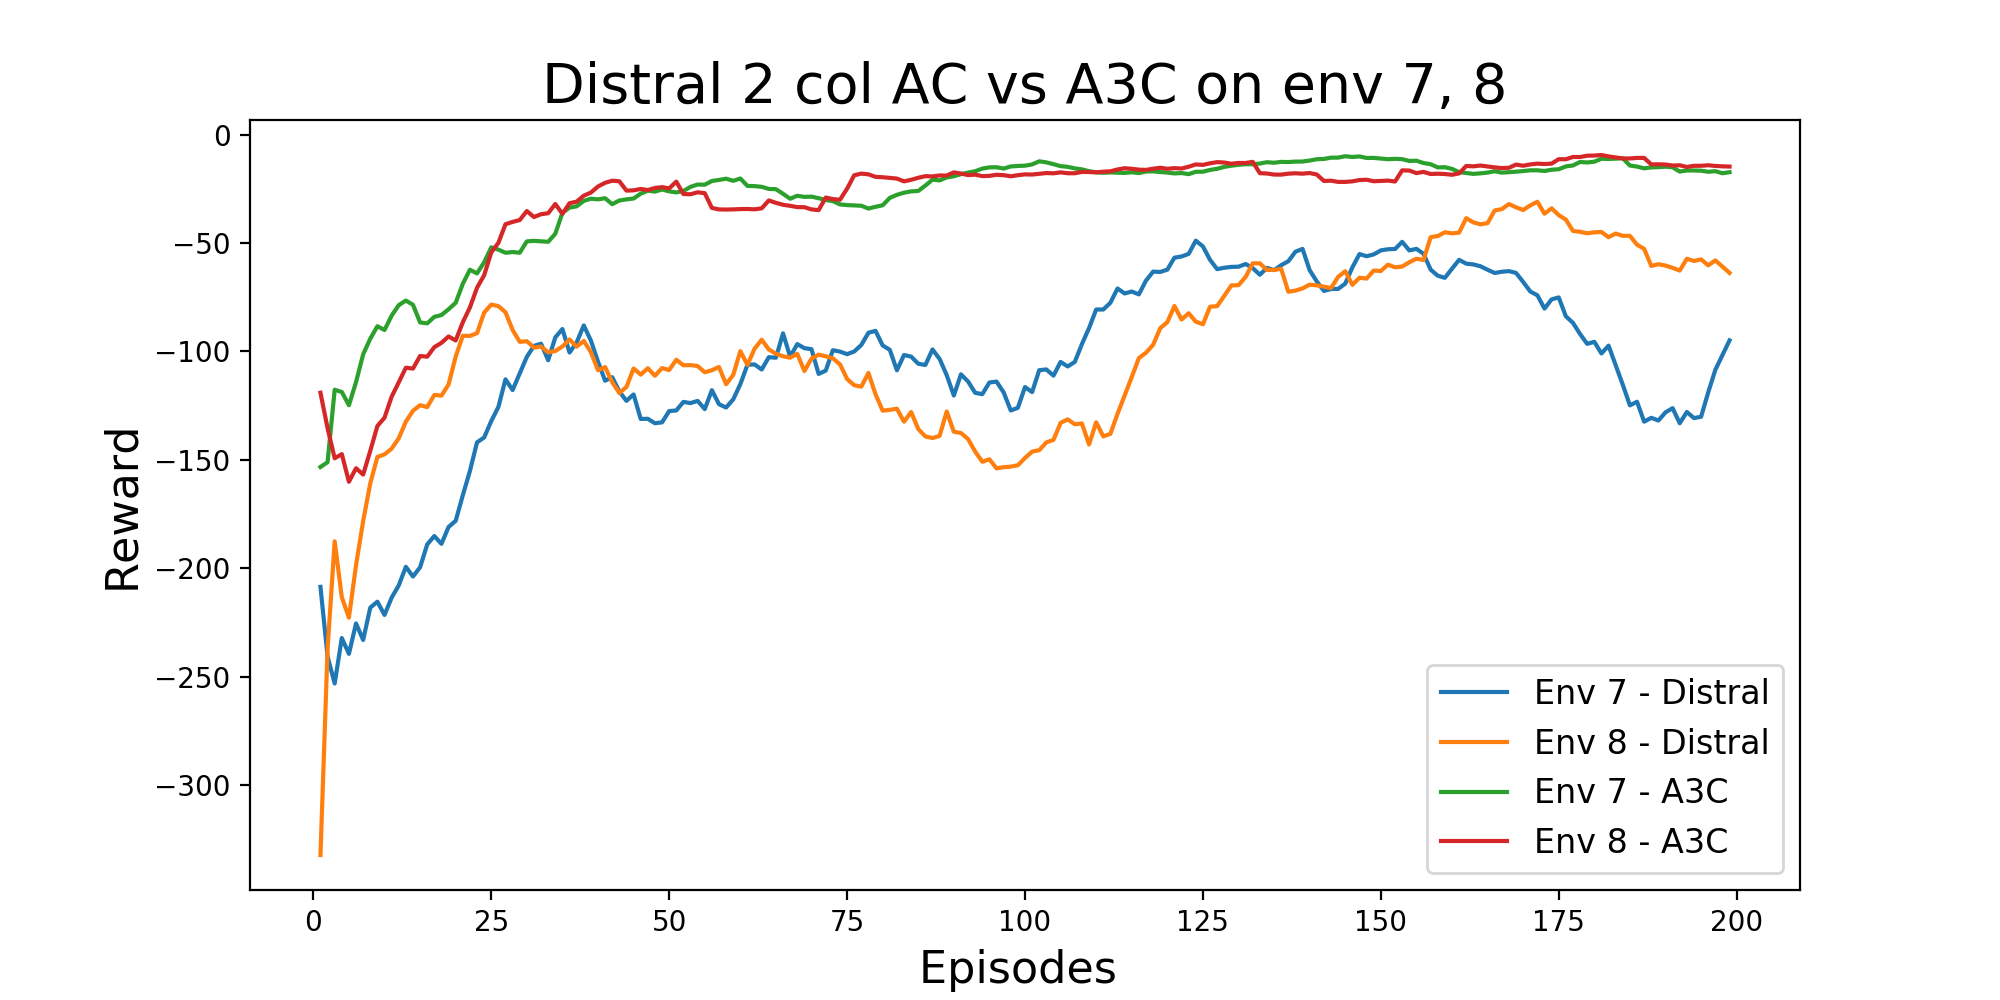
\includegraphics[width=\textwidth]{figs/d2_col_ac/d2_col_ac_7_8_rwd.png}
\end{minipage}%
\centering
\begin{minipage}{.5\textwidth}
\centering
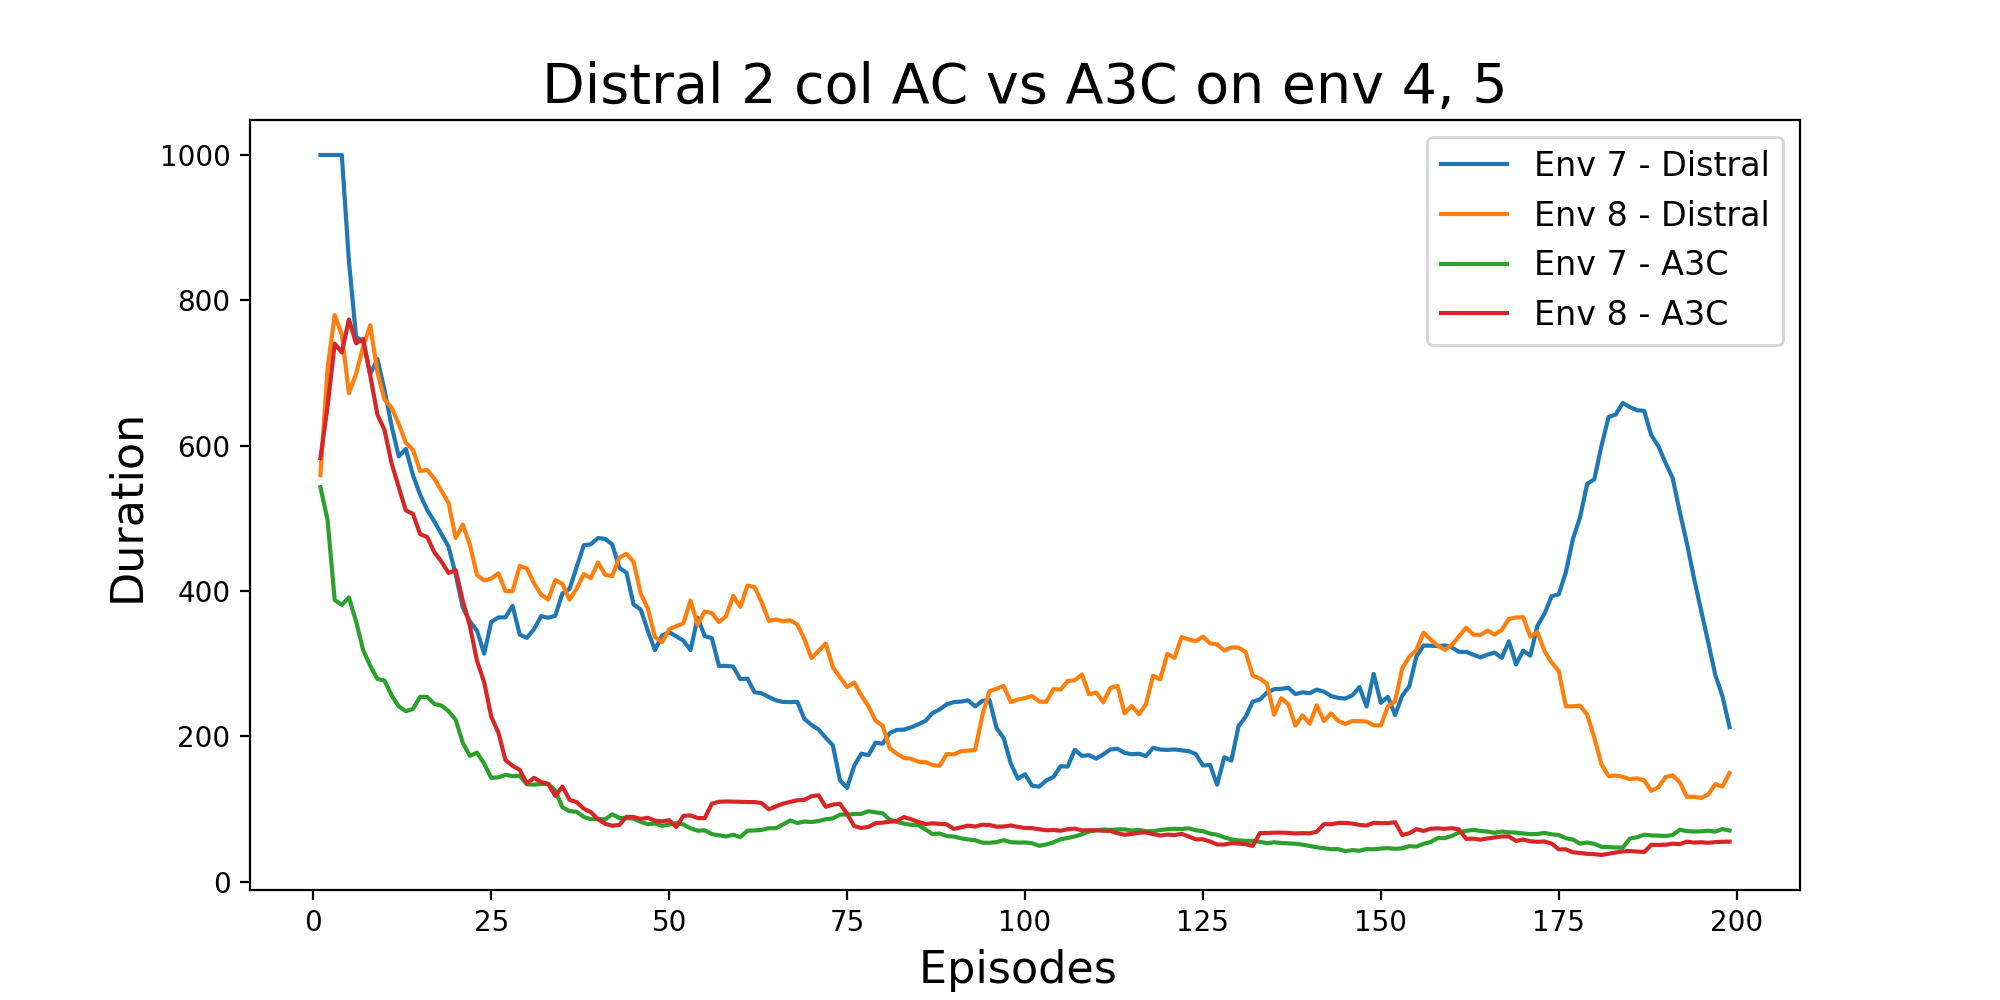
\includegraphics[width=\textwidth]{figs/d2_col_ac/d2_col_ac_7_8_dur.png}
\end{minipage}%
\end{figure}
Here we see that the algorithm did not solve either of the environments. Again, the algorithm appears to have numerical stability issues consistent to the results for environments 4 and 5, and the behaviour of Distral 1 col AC.

\subsubsection{Environments 4, 5 and 7}
\begin{figure}[H]
\centering
\begin{minipage}{.5\textwidth}
\centering
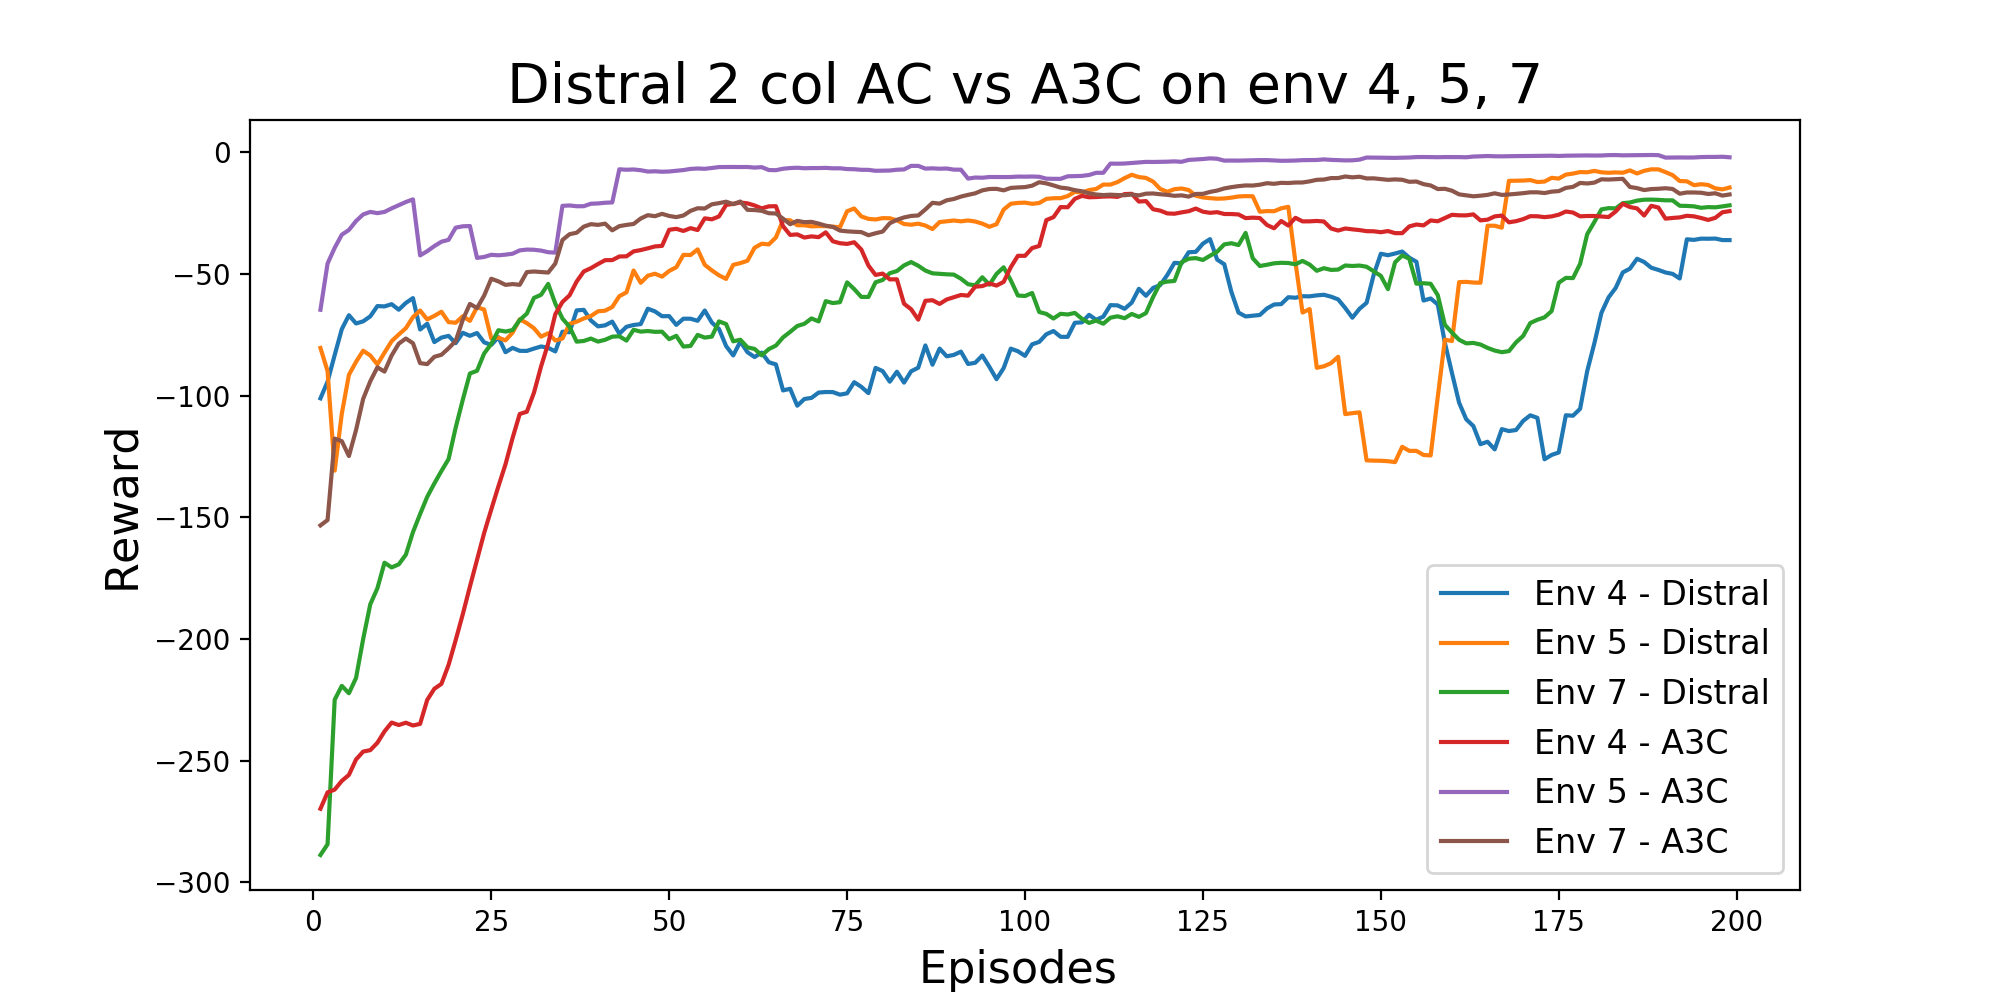
\includegraphics[width=\textwidth]{figs/d2_col_ac/d2_col_ac_4_5_7_rwd.png}
\end{minipage}%
\centering
\begin{minipage}{.5\textwidth}
\centering
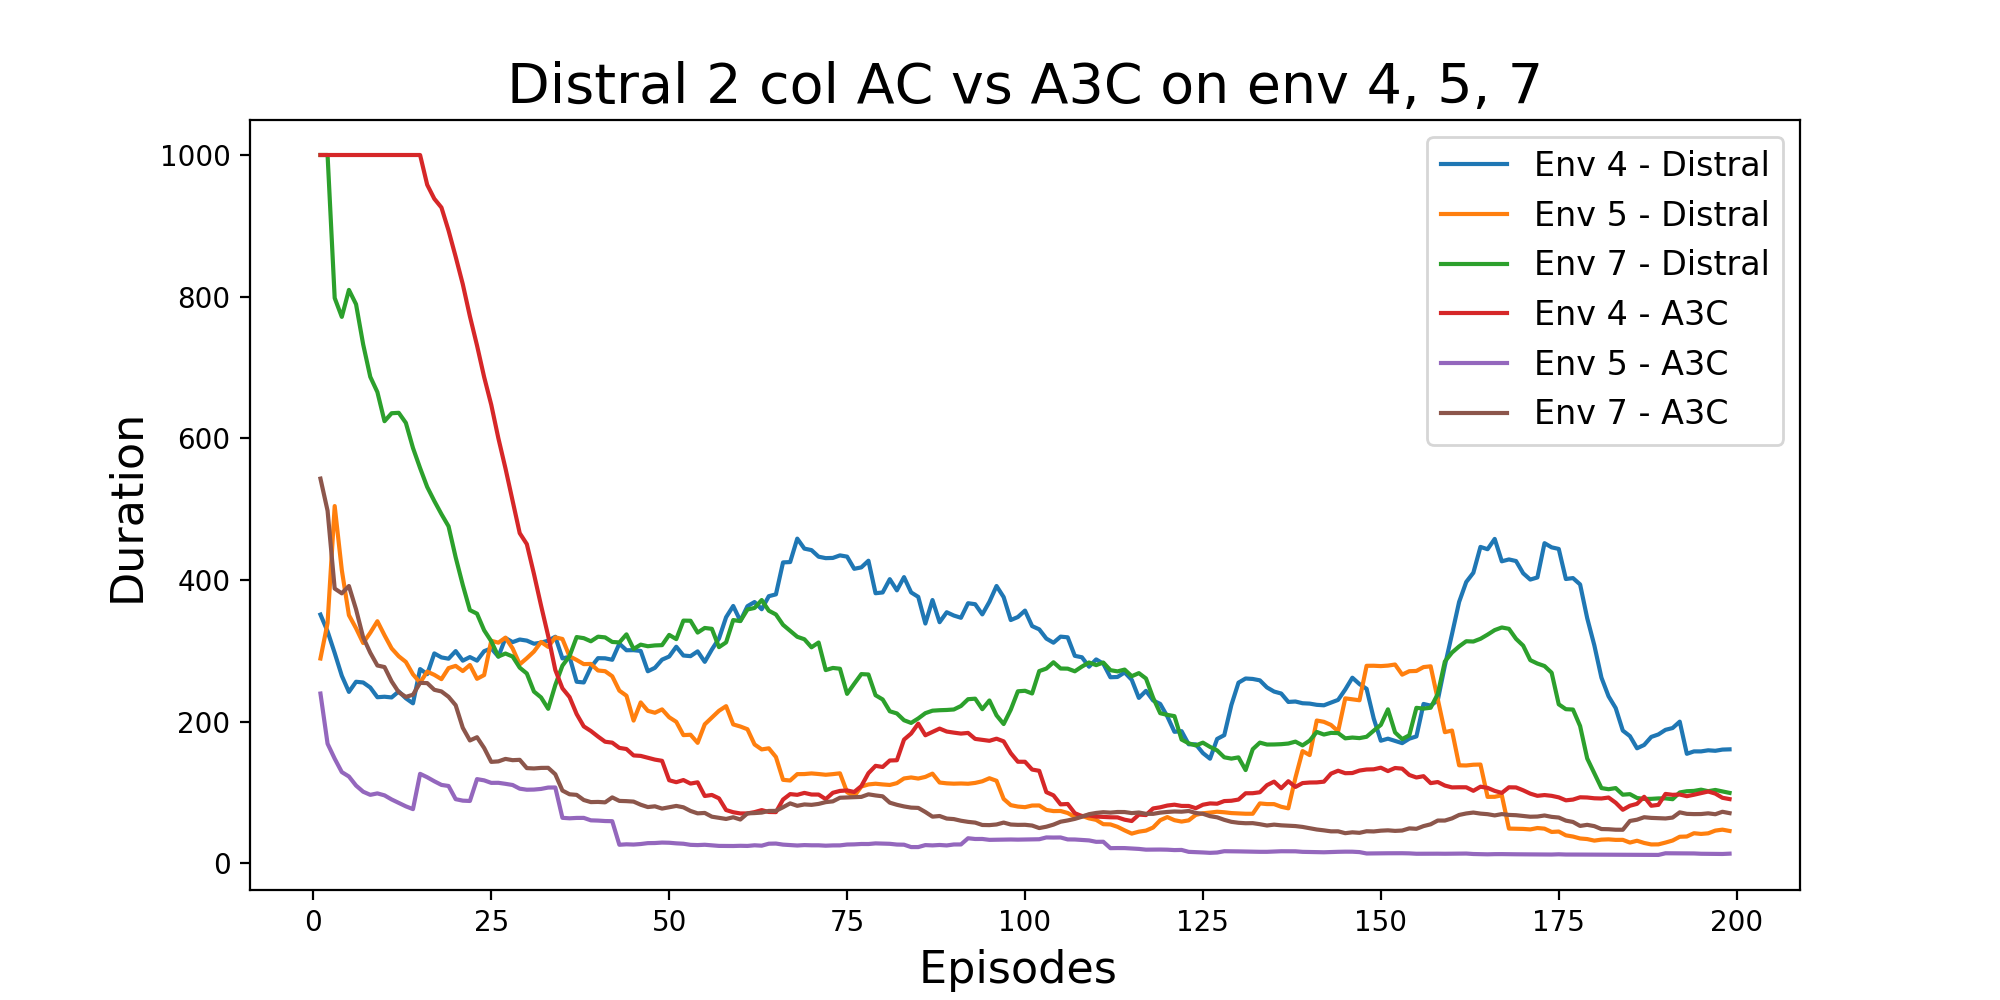
\includegraphics[width=\textwidth]{figs/d2_col_ac/d2_col_ac_4_5_7_dur.png}
\end{minipage}%
\end{figure}

\subsubsection{Environments 4, 5, 6, 7, 8}
\begin{figure}[H]
\centering
\begin{minipage}{.5\textwidth}
\centering
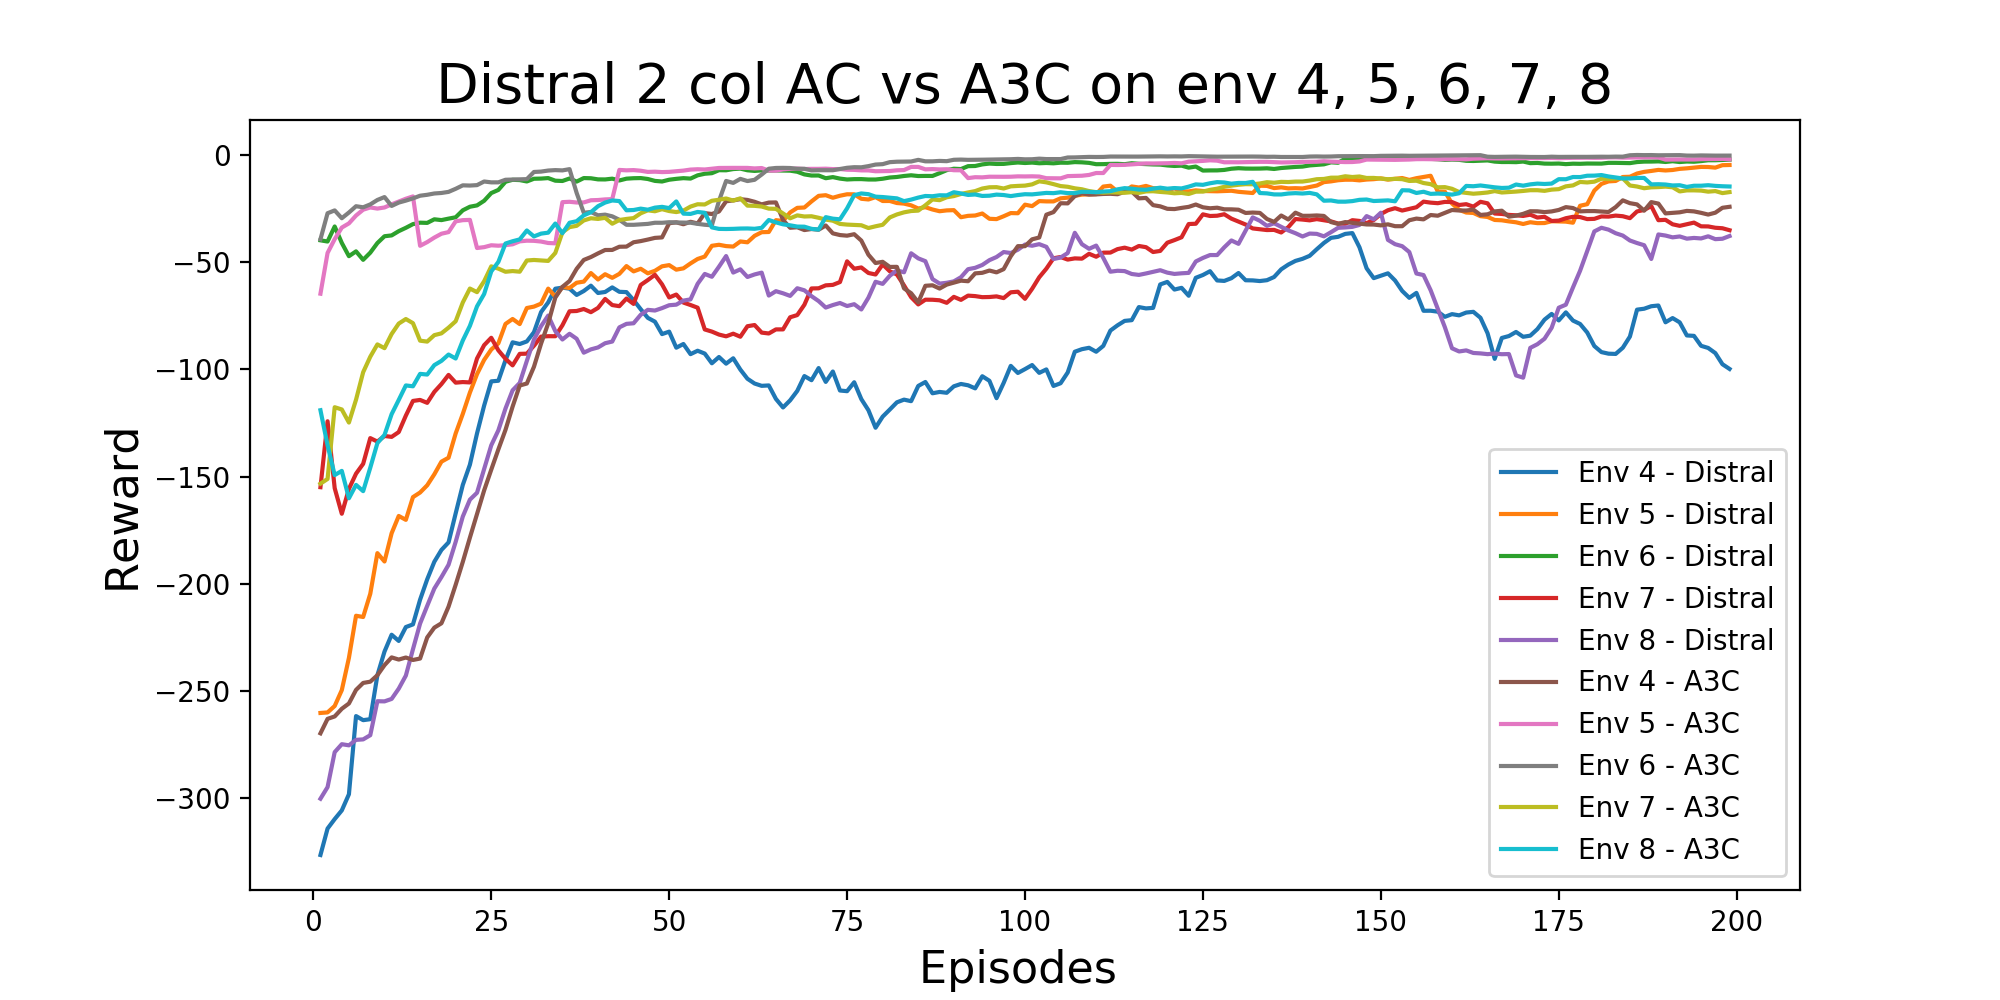
\includegraphics[width=\textwidth]{figs/d2_col_ac/d2_col_ac_4_5_6_7_8_rwd.png}
\end{minipage}%
\centering
\begin{minipage}{.5\textwidth}
\centering
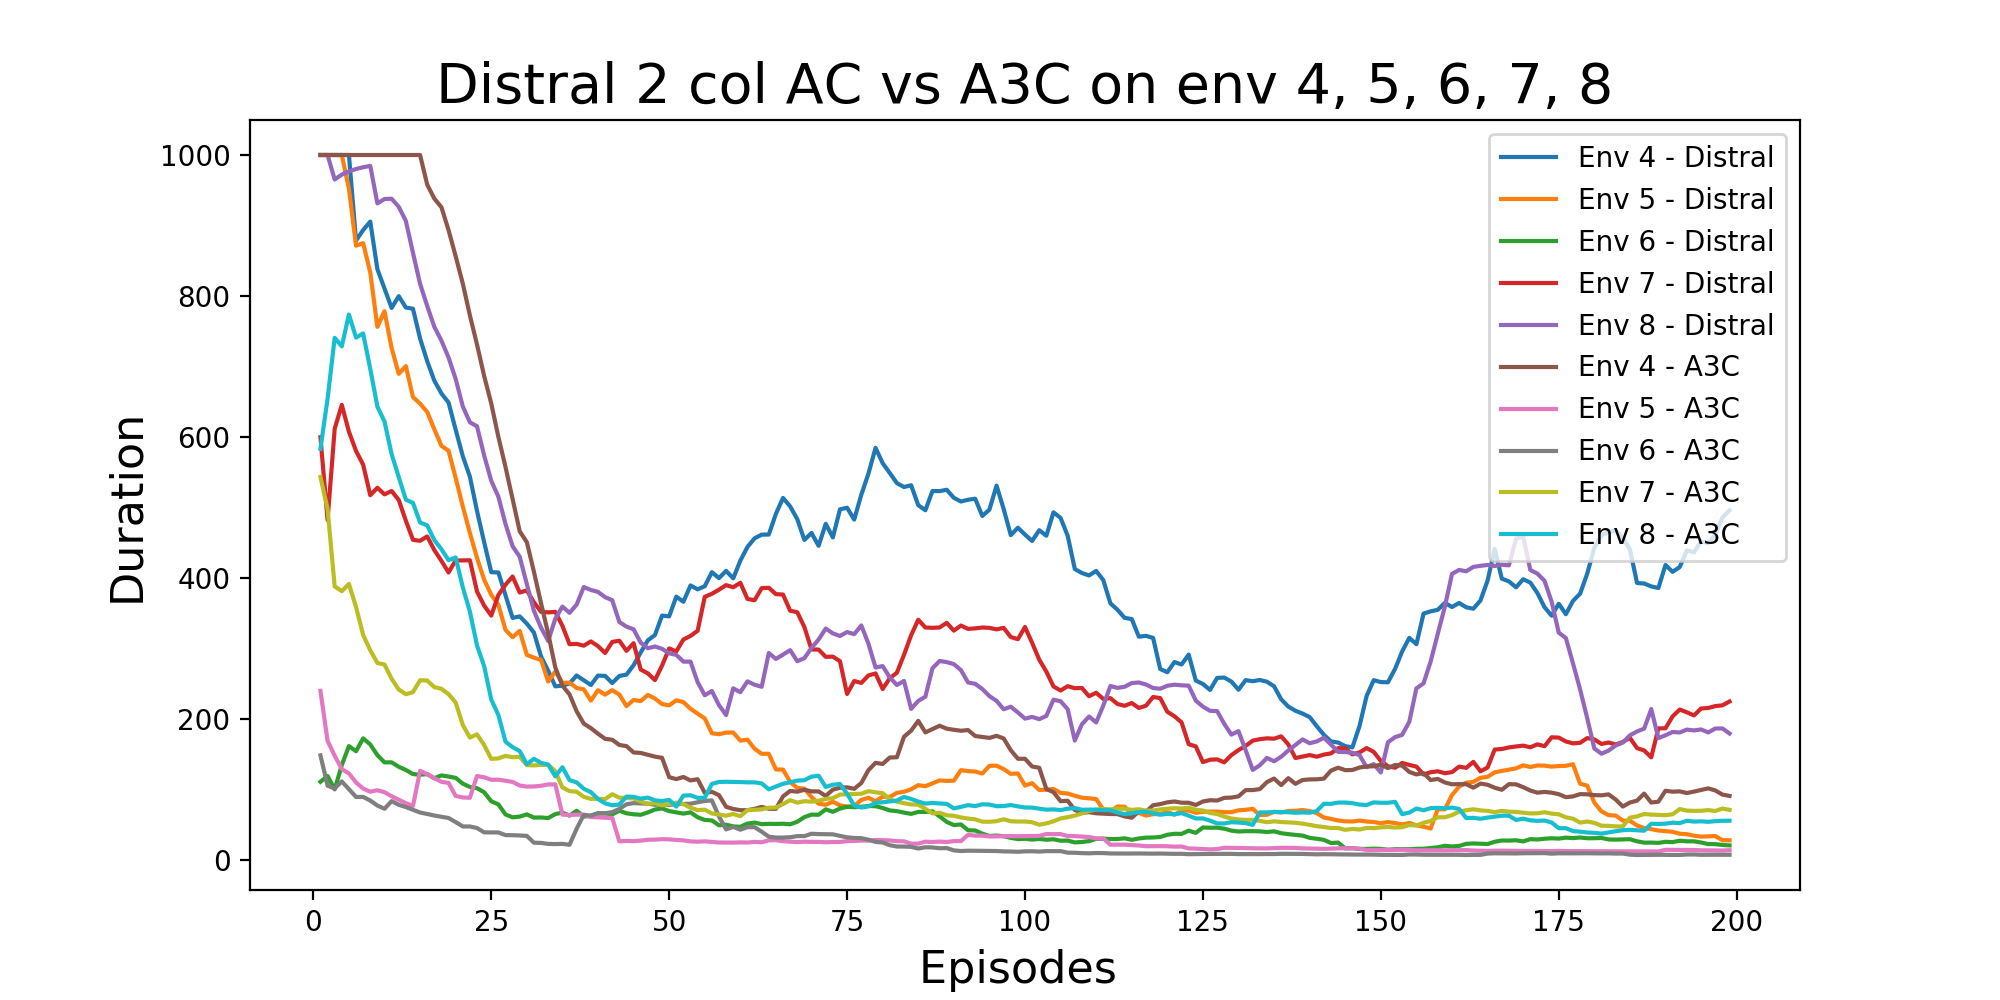
\includegraphics[width=\textwidth]{figs/d2_col_ac/d2_col_ac_4_5_6_7_8_dur.png}
\end{minipage}%
\end{figure}


\section{Distral 1 col vs Distral 2 col}

To assess the overall performance of all Distral algorithms across different architectures, we plot the average rewards and duration across environments 4 to 8

\begin{figure}[H]
\centering
\begin{minipage}{.5\textwidth}
\centering
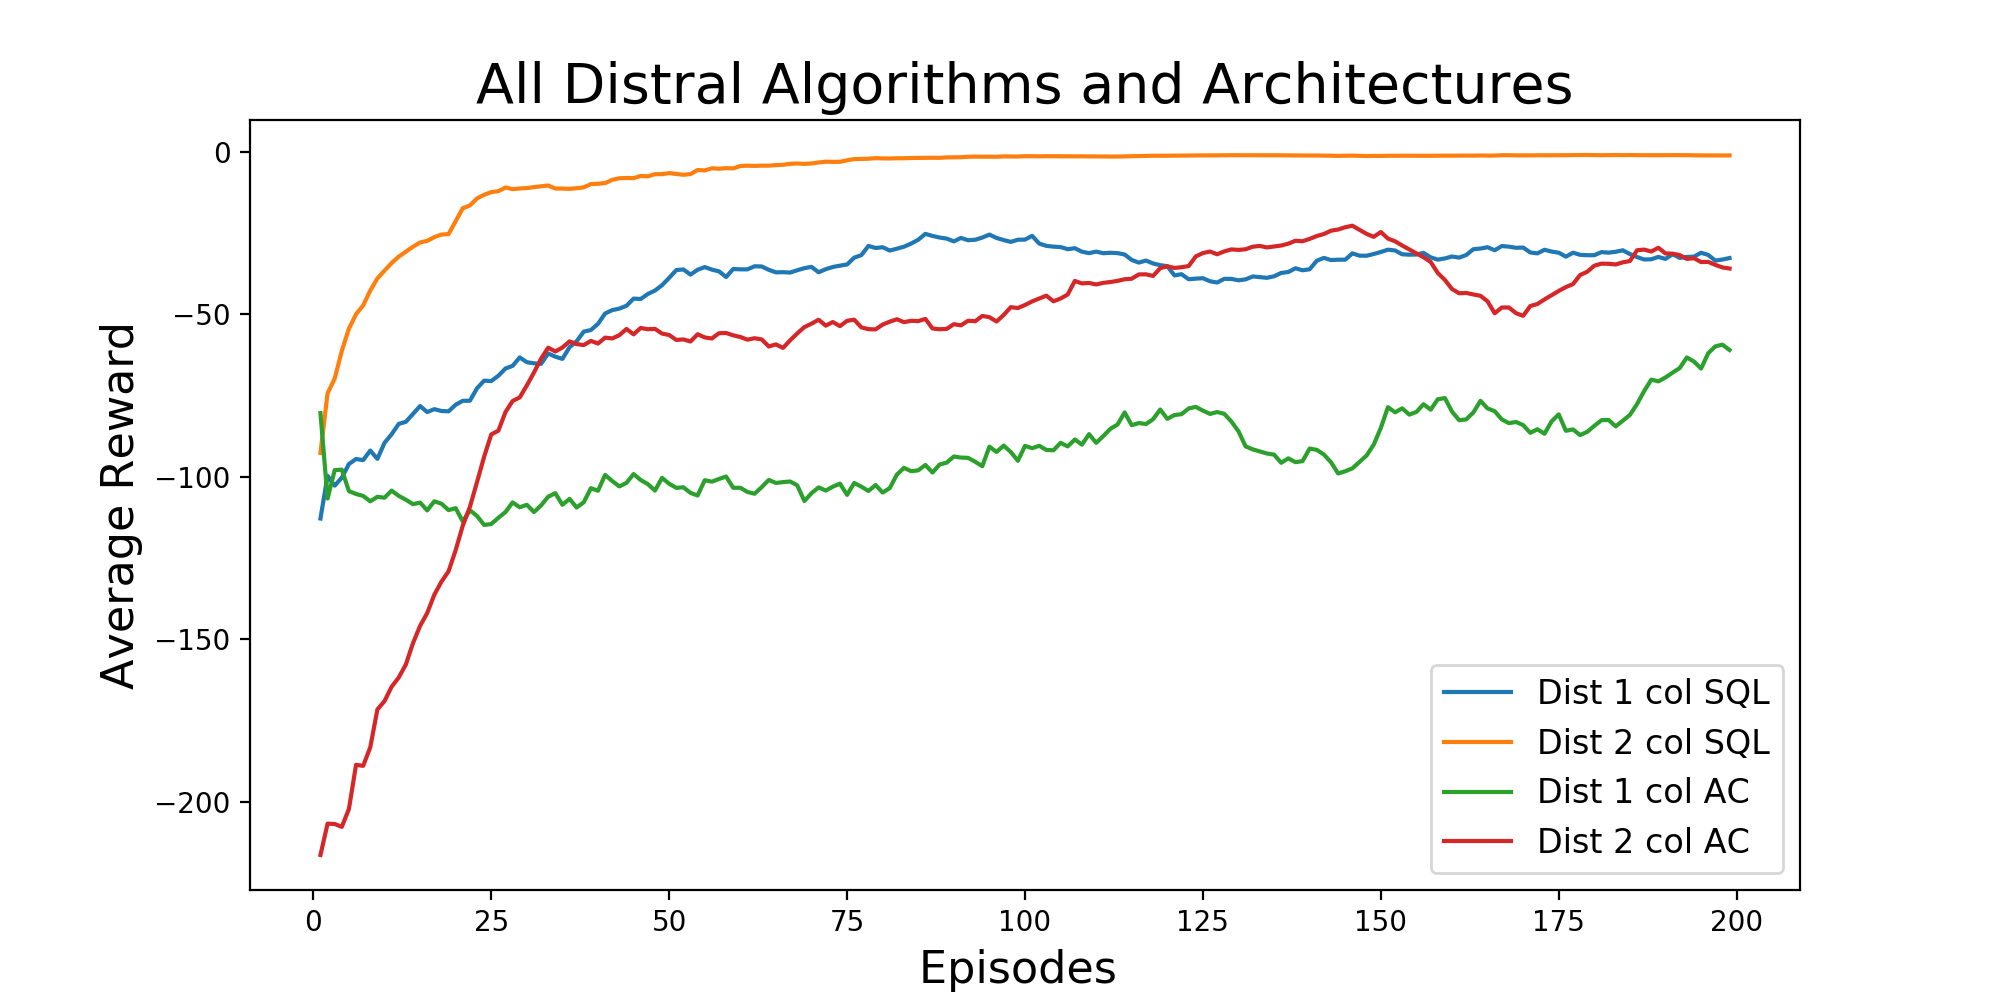
\includegraphics[width=\textwidth]{figs/all_algos_rwd.png}
\end{minipage}%
\centering
\begin{minipage}{.5\textwidth}
\centering
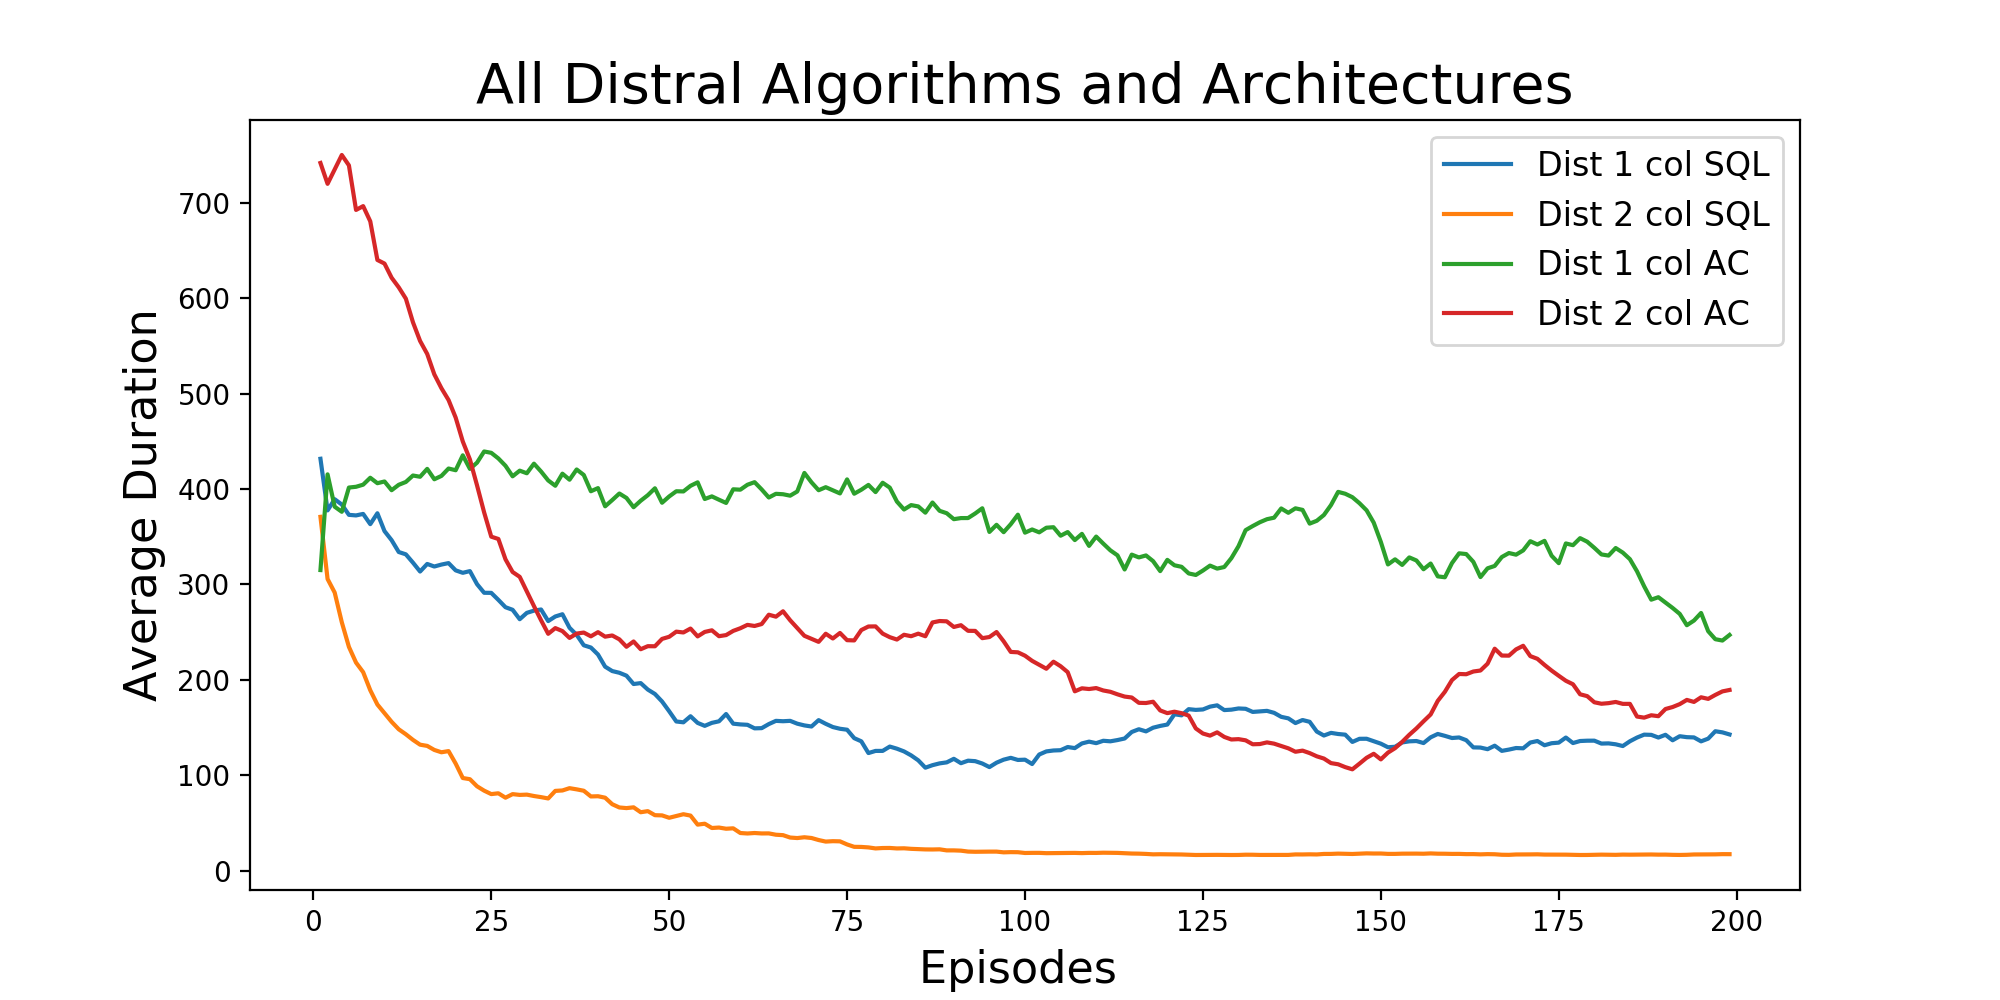
\includegraphics[width=\textwidth]{figs/all_algos_dur.png}
\end{minipage}%
\end{figure}

As shown above, Distral 2 columns implemented via SQL is by far the most effective algorithm comparing to other variants. Several reasons can be considered in order to explain this phenomenon. First, the difference in performance between Distral 1 col and Distral 1 col in both frameworks is likely due to the fact that the architecture of Distral 2 col defines task-specific policy in terms of the distilled policy. Specifically, recall that the task-specific policy defined in Distral 2 col is 
\begin{align}
\hat{\pi}_i(a_t|s_t) &= \frac{\exp(\alpha h_{\theta_0}(a_t| s_t) + \beta f_{\theta_i}(a_t | s_t))}{\sum_{a^\prime}\exp(\alpha h_{\theta_0}(a^\prime_t | s_t) + \beta f_{\theta_i}(a^\prime _t | s_t))} \nonumber
\end{align}
whereas the task-specific policy in Distral 1 is simply softmax over the logits $f_{\theta_i}(a_t | s_t)$. This gives Distral 1 col a significant disadvantage as the rewards are defined in terms of both the task-specific and distilled policies. Furthermore, both the regularized rewards and the distilled policy are used to optimize the task-specific policy respectively in the SQL and regularized AC frameworks.











\chapter{Conclusion and Suggestions on Further Work}

can use SQL plus DQN framework as mentioned in the rainbow paper \cite{hessel2018rainbow}\\

can integrate the Distral algorithms with SAC instead of regularized policy gradient, as mentioned in \cite{haarnoja2018soft}\\

can scale up experiments and train on deepmind lab\\

in all the other experiments done by deepmind in the depmind lab, Distral 2 col consistently outperform Distral 1 col, so don't know why we need distral 1 col in the first place?

\appendix

\bibliographystyle{plain}
\bibliography{references}

\chapter{Figures, tables and pseudocode}

Here are the gridworld environments taken from the \textbf{github project}. All environments except 1, 2, and 3 are identical to the environment demonstrated in the original work \cite{teh2017distral}:
\begin{figure}[H]
    \center
    \includegraphics[width=0.7\linewidth]{figs/GridWorlds.png}
    \caption{GridWorlds taken from the \textbf{github project}}
    \label{fig:gridworlds}
\end{figure}
\begin{figure}[H]
    \center
    \includegraphics[width=0.45\linewidth]{figs/distral1_2_diagram.png}
    \caption{Visual representation of differences between Distral 1 col vs Distral 2 col}
    \label{fig:distral12}
\end{figure}
\begin{figure}[H]
    \centering
    \includegraphics[width=0.85\linewidth]{figs/SAC.png}
    \caption{Pseudocode \cite{spinningupRL} for Soft Actor-Critic in the context of continuous action spaces}
    \label{fig:SAC}
\end{figure}


% \chapter{Code Listing}

% \begin{align}
% \label{line1} A=B\wedge B=C&\rightarrow A=C\\
% &\rightarrow C=A\\
% \intertext{note that}
% n!&=\prod_{1\leq i\leq n}i \\
% \int_{x=1}^y \frac 1 x \mathrm{d}x&=\log y
% \end{align}
% We can refer to labels like this \eqref{line1}. 
% Often lots of citations here (and elsewhere), e.g. \cite{Rey:D} or \cite[Theorem 2.3]{PriorNOP70}.
% \begin{definition}\label{def}
% See definition~\ref{def}.
% \end{definition}
% \begin{theorem}
% For all $n\in\nats,\; 1^n=1$.
% \end{theorem}
% \begin{proof}
% By induction over $n$.
% \end{proof}

\end{document}